\chapter{Pure shift NMR}
\label{chpt:pureshift}

\textit{Pure shift} NMR refers to the technique of acquiring NMR spectra free of multiplet structure, such that every chemical environment gives rise to a singlet.\autocite{Zangger2015PNMRS,Castanar2017MRC}
In the context of this thesis, we use the term `pure shift' exclusively to refer to broadband homodecoupled \proton{} spectra.
Here, `broadband' means that the couplings are removed from the entire spectrum, as opposed to just a subset of it (which can be accomplished through band-selective refocusing).
`Homodecoupled' refers to the fact that the primary target here is the removal of homonuclear couplings, which cannot be done simply through decoupling during acquisition.
Finally, although pure shift techniques can be applied to any nuclide, \proton{} spectra are of greatest interest because of the narrow chemical shift range of \proton{} which often leads to peak overlap.
(Another prominent case is \carbon{} pure shift NMR in isotopically enriched molecules, but this is not within the scope of this thesis.)

In this chapter, I first cover the theory underpinning, and a brief history of, pure shift experiments.
I then describe a variety of approaches aimed at increasing the quality of pure shift experiments: this is measured both in terms of \textit{sensitivity} as well as \textit{purity}, i.e.\ the lack of spectral artefacts arising from imperfect decoupling.
In all cases, we compare these against the state-of-the-art PSYCHE pure shift method.
Finally, I end with a section discussing the combination of pure shift diffusion spectroscopy---formally a pseudo-3D experiment---with the use of ultrafast (single-scan) NMR techniques to collapse the diffusion dimension.
This project was carried out in collaboration with Jean-Nicolas Dumez (University of Nantes).

The work in this chapter has not been submitted for publication.

\section{Theoretical background}
\label{sec:pureshift__intro_theory}

In this section, I use a system with two weakly coupled spins $I_1$ and $I_2$ to illustrate the ideas behind pure shift NMR.
This means that $H_{\text{free},I} = \Omega_1 I_{1z} + \Omega_2 I_{2z} + 2\pi JI_{1z}I_{2z}$; this is diagonal in the Zeeman basis:
\begin{equation}
    \label{eq:h_free_weak}
    H_\text{free} = \begin{pmatrix}
        \omega_{\alpha\alpha} & 0 & 0 & 0 \\
        0 & \omega_{\alpha\beta} & 0 & 0 \\
        0 & 0 & \omega_{\beta\alpha} & 0 \\
        0 & 0 & 0 & \omega_{\beta\beta} \\
    \end{pmatrix},
\end{equation}
where $\omega_{\lambda\mu} = \braket{\lambda\mu|H_{\text{free},I}|\lambda\mu}$ represents the precession frequency of the state $\ket{\lambda\mu}$.
Given that $I_z\ket{\alpha} = (1/2)\ket{\alpha}$ and $I_z\ket{\beta} = -(1/2)\ket{\beta}$, these are relatively easy to work out:
\begin{equation}
    \label{eq:state_precessions}
    \begin{aligned}
        \omega_{\alpha\alpha} &= \frac{1}{2}(\Omega_1 + \Omega_2 + \pi J) &
        \omega_{\alpha\beta} &= \frac{1}{2}(\Omega_1 - \Omega_2 - \pi J) \\
        \omega_{\beta\alpha} &= \frac{1}{2}(-\Omega_1 + \Omega_2 - \pi J) &
        \omega_{\beta\beta} &= \frac{1}{2}(-\Omega_1 - \Omega_2 + \pi J).
    \end{aligned}
\end{equation}
The corresponding propagator for a time $\tau$, $U = \exp(-\mi H_{\text{free},I}\tau)$, is then just:
\begin{equation}
    \label{eq:u_free_weak}
    U = \begin{pmatrix}
        \exp(-\mi\omega_{\alpha\alpha}\tau) & 0 & 0 & 0 \\
        0 & \exp(-\mi\omega_{\alpha\beta}\tau) & 0 & 0 \\
        0 & 0 & \exp(-\mi\omega_{\beta\alpha}\tau) & 0 \\
        0 & 0 & 0 & \exp(-\mi\omega_{\beta\beta}\tau) \\
    \end{pmatrix}.
\end{equation}

In the previous chapter, we showed how pulse sequences could be analysed using two different bases for spin-\half{} systems, depending on which was most mathematically expedient.
To analyse pure shift NMR it turns out to be most convenient to introduce a third basis, namely $\{I_\alpha, I_\beta, I_+, I_-\}$\autocite{Keeler2010,Thrippleton2005JMR,Griesinger1986JCP}.
The definitions of these were given in \cref{eq:other_single_spin_ops}: it is clear from there that these represent single matrix elements of $\rho$ when expressed in the Zeeman basis.
The same is true of their products in systems containing multiple spins.
Consequently, the evolution of these operators under $H_{\text{free},I}$ is extraordinarily simple to calculate in matrix form: for example, we have that
\begin{equation}
    \label{eq:single_elem_plusalpha_evolution}
    I_{1+}I_{2\alpha} = \begin{pmatrix}
        0 & 0 & 1 & 0 \\
        0 & 0 & 0 & 0 \\
        0 & 0 & 0 & 0 \\
        0 & 0 & 0 & 0 \\
    \end{pmatrix},
\end{equation}
so $U(\tau) I_{1+} I_{2\alpha} \adj{U}(\tau)$ is simply
\begin{equation}
    \label{eq:single_elem_plusalpha_evolution_2}
    \begin{pmatrix}
        0 & 0 & \exp(-\mi\omega_{\alpha\alpha}\tau)\exp(\mi\omega_{\beta\alpha}\tau) & 0 \\
        0 & 0 & 0 & 0 \\
        0 & 0 & 0 & 0 \\
        0 & 0 & 0 & 0 \\
    \end{pmatrix} = \exp[-\mi(\Omega_1 + \pi J)\tau] I_{1+}I_{2\alpha}.
\end{equation}
Essentially, all of these operators evolve into themselves under $H_{\text{free},I}$, while acquiring a phase factor which depends on the difference between two of the frequencies.
The rules for the single-quantum operators on spin 1 are explicitly given here:
\begin{align}
    I_{1+}I_{2\alpha} &\longrightarrow \exp[-\mi(\Omega_1 + \pi J)\tau] I_{1+}I_{2\alpha} \label{eq:shift_basis_evolution_pa} \\
    I_{1+}I_{2\beta} &\longrightarrow \exp[-\mi(\Omega_1 - \pi J)\tau] I_{1+}I_{2\beta} \label{eq:shift_basis_evolution_pb} \\
    I_{1-}I_{2\alpha} &\longrightarrow \exp[\mi(\Omega_1 + \pi J)\tau] I_{1-}I_{2\alpha} \label{eq:shift_basis_evolution_ma} \\
    I_{1-}I_{2\beta} &\longrightarrow \exp[\mi(\Omega_1 - \pi J)\tau] I_{1-}I_{2\beta} \label{eq:shift_basis_evolution_mb}
\end{align}
The rules for the corresponding operators on spin 2 can be easily obtained by permutation of labels.
Notice that the evolution frequencies of the $-1$-quantum operators each correspond to one peak of the multiplet: for example, $\Omega_1 + \pi J$ and $\Omega_1 - \pi J$ (\cref{eq:shift_basis_evolution_ma,eq:shift_basis_evolution_mb}) correspond to the two peaks of the spin-1 doublet.

Consider now a simple spin echo sequence, $90^\circ_{x}$--$\tau$--$180^\circ_{x}$--$\tau$--detection.
The initial excitation pulse acts on both spins 1 and 2, and thus generates a mixture of all eight possible single-quantum operators (the four above plus four more on spin 2).
For simplicity, we only consider the $I_{1+}I_{2\alpha}$ term.
This evolves in the first $\tau$ delay to give $\exp[-\mi(\Omega_1 + \pi J)\tau] I_{1+}I_{2\alpha}$.
The $180^\circ$ pulse \textit{flips} both spins 1 and 2, in that it causes the transitions $I_+ \leftrightarrow I_-$ and $I_\alpha \leftrightarrow I_\beta$; consequently, we have that
\begin{equation}
    \label{eq:spin_echo_1}
    \exp[-\mi(\Omega_1 + \pi J)\tau] I_{1+}I_{2\alpha} \longrightarrow \exp[-\mi(\Omega_1 + \pi J)\tau] I_{1-}I_{2\beta}.
\end{equation}
In the second delay, we get a second phase factor from the evolution of the $I_{1-}I_{2\beta}$ operator:
\begin{align}
    \label{eq:spin_echo_2}
    \exp[-\mi(\Omega_1 + \pi J)\tau] I_{1-}I_{2\beta} \longrightarrow
    &\exp[-\mi(\Omega_1 + \pi J)\tau] \exp[\mi(\Omega_1 - \pi J)\tau] I_{1-}I_{2\beta} \notag \\
    = &\exp(-2\mi \pi J\tau) I_{1-}I_{2\beta}.
\end{align}
Detection of this gives us one of the two peaks of the spin-1 doublet, as described previously, but with a phase factor tacked on.
The $\Omega_1$ terms in the phase factor are cancelled out, which reflects the fact that the offset (or chemical shift) is refocused by the $180^\circ$ pulse.
However, the J-evolution is not refocused, which leads to characteristic phase distortions in the detected multiplets.
The same is true of all the other single-quantum operators on both spins.

In order to refocus the J-evolution as well as the chemical shift, we would need---instead of a $180^\circ$ pulse---a pulse sequence element which simultaneously effects \textit{all} of the following transitions:
\begin{align}
    I_{1+}I_{2\alpha} \longrightarrow I_{1-}I_{2\alpha}; \quad I_{1+}I_{2\beta} \longrightarrow I_{1-}I_{2\beta}; \quad
    I_{1-}I_{2\alpha} \longrightarrow I_{1+}I_{2\alpha}; \quad I_{1-}I_{2\beta} \longrightarrow I_{1+}I_{2\beta}; \label{eq:pure_shift_requirement_spin1} \\
    I_{1\alpha}I_{2+} \longrightarrow I_{1\alpha}I_{2-}; \quad I_{1\beta}I_{2+} \longrightarrow I_{1\beta}I_{2+}; \quad
    I_{1\alpha}I_{2-} \longrightarrow I_{1\alpha}I_{2+}; \quad I_{1\beta}I_{2-} \longrightarrow I_{1\beta}I_{2-}. \label{eq:pure_shift_requirement_spin2}
\end{align}
Such an element forms the basis of a pure shift technique, and I refer to it here as a \textit{pure shift element} (PSE).
The difficulty in designing a PSE is that \textit{all} spins must be simultaneously decoupled from each other (and not just one spin).
For example, if we only had to invert spin 1 and not spin 2 (i.e.\ only \cref{eq:pure_shift_requirement_spin1} and not \cref{eq:pure_shift_requirement_spin2}), this could be trivially accomplished by a selective $180^\circ$ pulse on spin 1.
However, this would not bring about the correct transitions for spin 2.
Yet another complicating factor is that the spins will have offsets and couplings which are \textit{a priori} not known; so the design of the PSE cannot use such parameters as inputs.
These limitations mean that it is impossible to accomplish the above transitions \textit{in full}; rather, a more realistic scenario involves
\begin{equation}
    \label{eq:realistic_pse}
    I_{1+}I_{2\alpha} \longrightarrow c I_{1-}I_{2\alpha} + \sum_i c'_i M_i
\end{equation}
and likewise for the other operators.
Here, the desired transition probability $c$ directly correlates with the sensitivity of the PSE, and the $M_i's$ are some other undesired operators which (if detectable) must either be suppressed or generate artefacts in the spectrum.

In the above discussion, note that the role of the PSE is to invert the $I_+$ and $I_-$ terms, and to retain the $I_\alpha$ and $I_\beta$ terms.
The prevailing terminology is to refer to the spins with $I_+$ and $I_-$ terms as \textit{active spins}, and the $I_\alpha$ and $I_\beta$ spins as \textit{passive spins}.
Thus, for example, in the context of \cref{eq:pure_shift_requirement_spin1}, spin 1 is active and spin 2 is passive.
The detected signal always arises from the active spins.

Before moving on to the discussion of how this is accomplished in practice, I insert a slight digression about \textit{J-resolved} (or \textit{2DJ}) \textit{spectroscopy}, which is very closely related to pure shift NMR.
The basic 2DJ sequence involves a spin echo of duration $t_1$ (i.e.\ the $\tau$ delay above is $t_1/2$), immediately followed by detection.
If we only consider a single operator and reuse the analysis above, then we have that
\begin{align}
    \label{eq:2dj_operator_analysis}
    I_{1+}I_{2\alpha} \xrightarrow[]{t_1/2} &\exp[-\mi(\Omega_1 + \pi J)t_1/2] I_{1+}I_{2\alpha} \notag \\
    \xrightarrow[]{180^\circ} &\exp[-\mi(\Omega_1 + \pi J)t_1/2] I_{1-}I_{2\beta} \notag \\
                      \xrightarrow[]{t_1/2} &\exp(-\mi \pi J t_1) I_{1-}I_{2\beta}.
\end{align}
This yields a complex signal of the form
\begin{equation}
    \label{eq:2dj_signal}
    s(t_1, t_2) = \exp(-\mathrm{i}\pi J t_1) \exp[\mi(\Omega_1 - \pi J) t_2],
\end{equation}
which when Fourier transformed yields a phase twist lineshape at $(-\pi J, \Omega_1 - \pi J)$.
The other component on spin 1 (starting from $I_{1+}I_{2\beta}$) likewise yields a phase twist at $(\pi J, \Omega_1 + \pi J)$.
It has long been known that \textit{shearing} this 2DJ spectrum by $45^\circ$ (i.e.\ moving each data point $(\Omega_1, \Omega_2)$ to $(\Omega_1, \Omega_2 - \Omega_1)$) generates a spectrum which only has chemical shift information in the $\omega_2$ dimension.
After magnitude-mode processing, projection of this spectrum onto the $\omega_2$ axis, for example, would in principle yield a pure shift spectrum.\footnote{Or equivalently, projection of the unsheared spectrum along a $45^\circ$ axis\autocite{Aue1976JCP}.}
This is true, but in practice the phase twist lineshapes cause the resulting resolution to be very poor, which defeats the purpose of using a pure shift spectrum.
To circumvent this issue, a glut of special processing techniques have been proposed\autocite{Xu1991JMR,Nuzillard1996JMRSA,Simova1997JMR} (see also references therein); but more ideally, we want a phase-sensitive 2DJ spectrum, where a pair of `echo' and `antiecho' signals are obtained:%
\footnote{The terms `echo' and `antiecho' refer to the relative senses of the coherences evolving during $t_1$ and $t_2$: in the echo spectrum these have opposite signs, e.g.\ $I_zS_+$ and $I_-$ in the HSQC, and in the antiecho spectrum they have the same sign. As pointed out by Pell and Keeler\autocite{Pell2007JMR}, this is not really appropriate for the 2DJ experiment since each half of $t_1$ has a coherence with a different sense, but we will stick to this nomenclature as the underlying concept is very similar to that of echo--antiecho processing.}
\begin{align}
    \label{eq:2dj_signal_ea}
    s_\text{echo}(t_1, t_2) &= \exp(-\mathrm{i}\pi J t_1) \exp[\mi(\Omega_1 - \pi J) t_2] \\
    s_\text{antiecho}(t_1, t_2) &= \exp(\mathrm{i}\pi J t_1) \exp[\mi(\Omega_1 - \pi J) t_2]
\end{align}
and processed in the same way as previously described in \cref{subsec:theory__2dnmr} to yield the double absorption-mode lineshape.
The echo signal is of course the same as in \cref{eq:2dj_signal}, but to obtain the antiecho signal, we require a different pulse sequence with a PSE inserted right before detection.
Note that we start with a different operator here, $I_{1-}I_{2\alpha}$, in order to end up with the same $I_{1-}I_{2\beta}$ operator just before detection.
\begin{align}
    \label{eq:2dj_signal_antiecho}
    I_{1-}I_{2\alpha} \xrightarrow[]{t_1/2} &\exp[\mi(\Omega_1 + \pi J)t_1/2] I_{1-}I_{2\alpha} \\
    \xrightarrow[]{180^\circ} &\exp[\mi(\Omega_1 + \pi J)t_1/2] I_{1+}I_{2\beta} \\
    \xrightarrow[]{t_1/2} &\exp(\mi \pi J t_1) I_{1+}I_{2\beta} \\
    \xrightarrow[]{\text{PSE}} &\,c \exp(\mi \pi J t_1) I_{1-}I_{2\beta}.
\end{align}
In order to apply echo--antiecho processing, the decrease in sensitivity by a factor of $c$ must also be applied to the echo spectrum: this can be done by simply inserting the PSE before the $t_1$ spin echo, which does not affect the relative modulation in $t_1$ and $t_2$.
Thus, we see that \textit{exactly the same PSE} allows us to generate pure shift spectra as well as absorption-mode 2DJ spectra, a fact which has been previously demonstrated using various PSEs.\autocite{Pell2007JMR,Foroozandeh2015CC}
In fact, the same formalism can be used to describe a family of small flip angle COSY experiments, including ECOSY\autocite{Griesinger1985JACS,Sorensen1985JACS,Griesinger1986JCP} and $z$-COSY\autocite{Oschkinat1986JMR,Pell2007MRC,Moutzouri2020ACIE}; these are also closely related to pure shift NMR.
In particular, the anti $z$-COSY experiment is a precursor to PSYCHE, and is analysed in \cref{subsec:pureshift__psyche_analysis}.
However, a full discussion of these is beyond the scope of this thesis.

\section{Pure shift in practice}
\label{sec:pureshift__intro_practice}

In the previous section, I described the underlying theory used for analysing PSEs and showed how such an element could be used to record absorption-mode 2DJ spectra.
From this, one can obtain a pure shift spectrum through shearing and projection.
However, this is only an \textit{indirect} route to a pure shift spectrum.
In this section, we will tackle the main question of how pure shift experiments may be \textit{directly} acquired using a PSE.
Following this, I cover several examples of PSEs reported in the literature.
This is not an exhaustive survey of pure shift methods: I only choose to cover a handful of PSEs which specifically accomplish the transformations listed in \cref{eq:pure_shift_requirement_spin1,eq:pure_shift_requirement_spin2}.
Thus, for example, constant-time techniques (which are widely used to suppress \carbon{}--\carbon{} couplings in labelled biomolecules) are not mentioned.

\subsection{Acquisition modes}
\label{subsec:pureshift__acquisition_modes}

\begin{figure}[htbp]
    \centering
    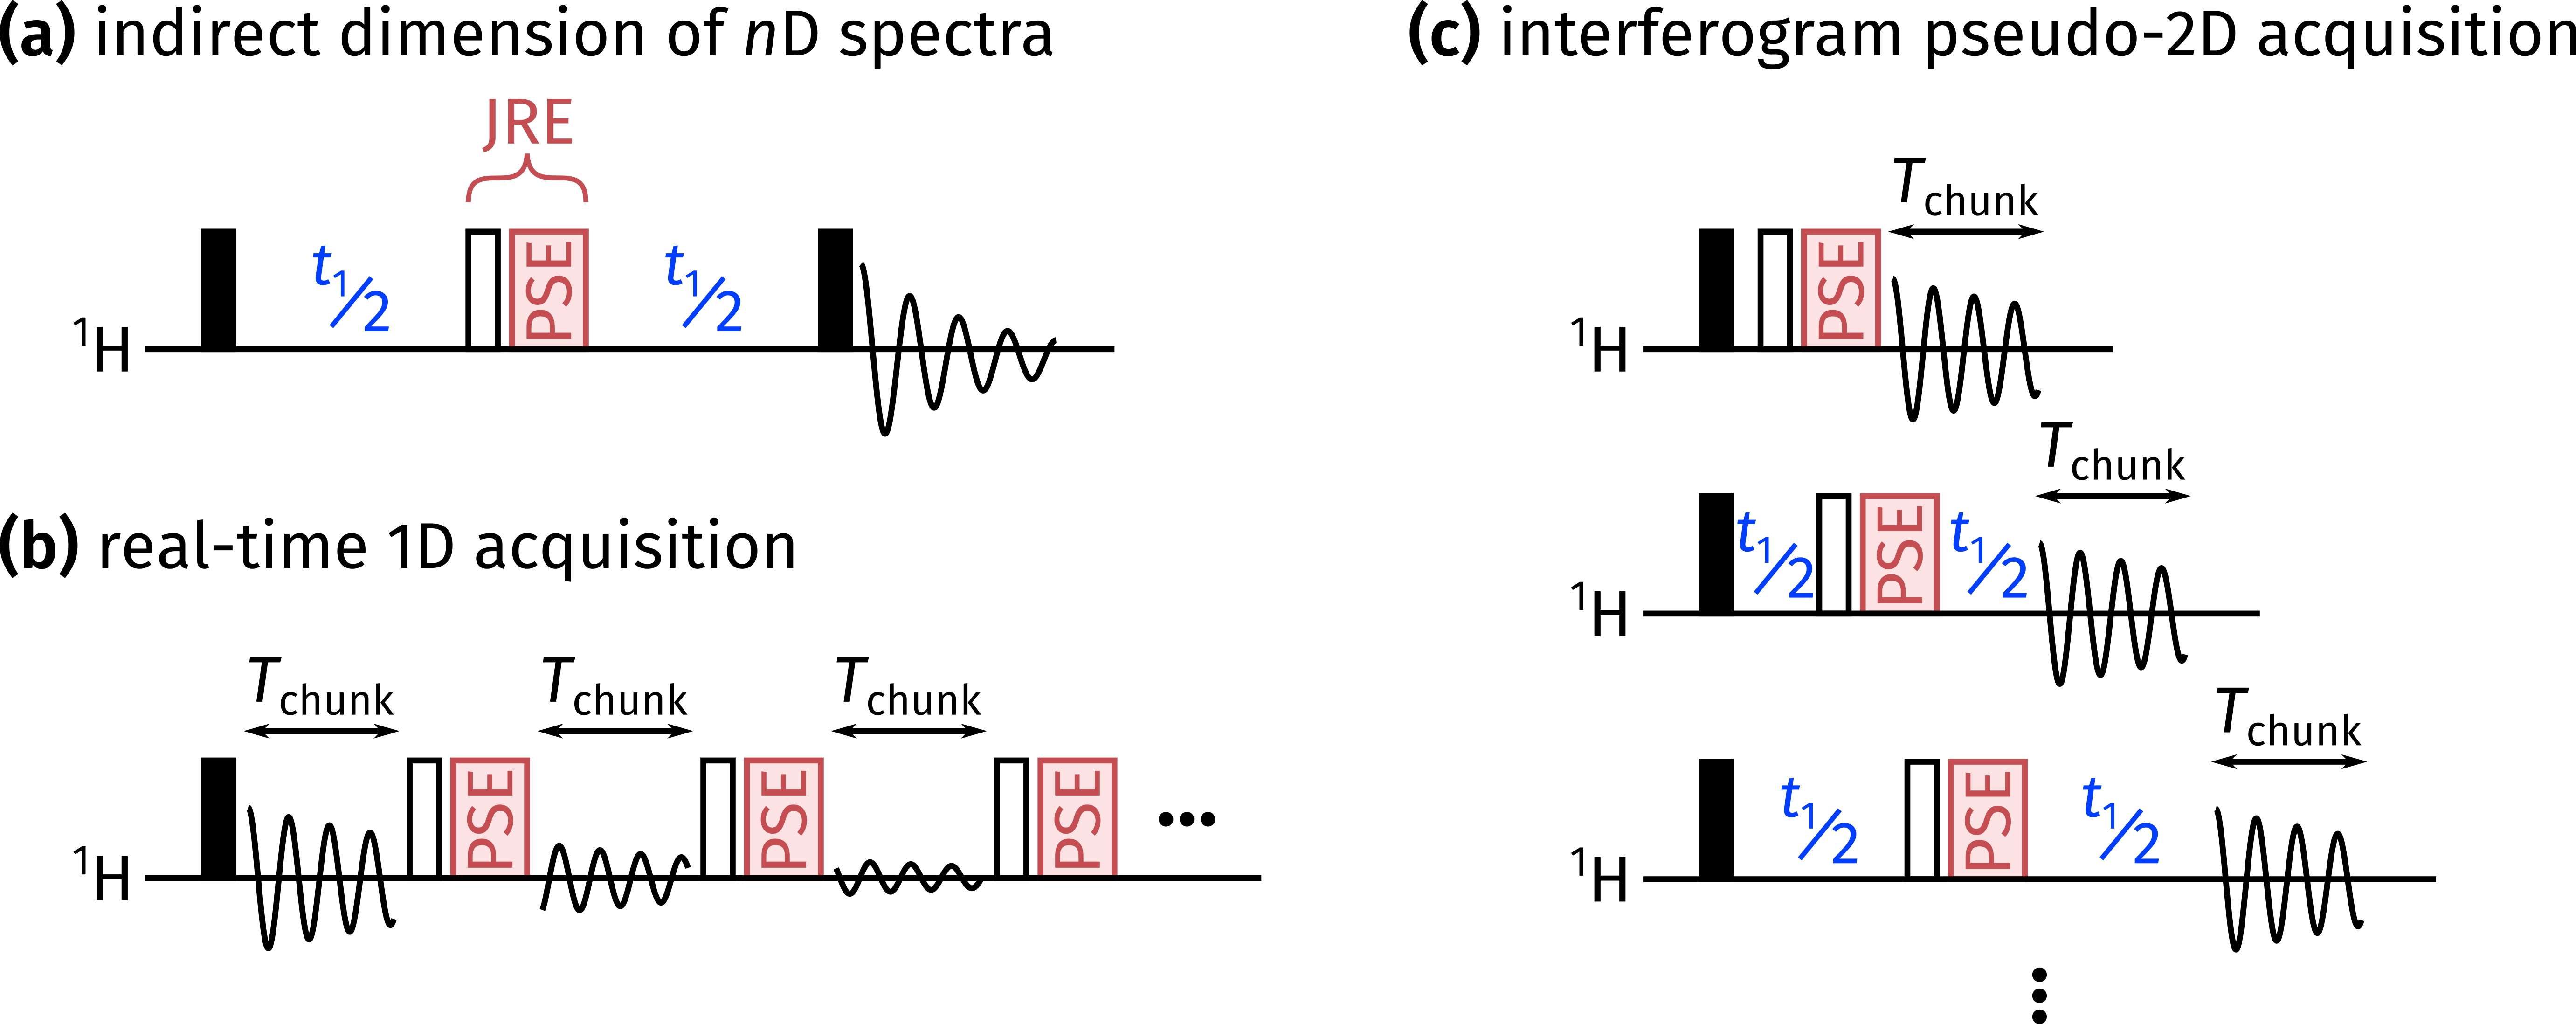
\includegraphics[]{pureshift/modes.png}%
    {\phantomsubcaption\label{fig:pureshift_modes_indirectnd}}%
    {\phantomsubcaption\label{fig:pureshift_modes_realtime}}%
    {\phantomsubcaption\label{fig:pureshift_modes_interferogram}}%
    \caption[Pure shift acquisition modes]{
        Possible acquisition modes for pure shift spectroscopy.
        The red box labelled `PSE' indicates a generic pure shift element, which can be any of those described in the main text.
        In practice, gradients are also used to suppress unwanted coherence transfers; these are not shown here for simplicity.
        \textbf{(\subref*{fig:pureshift_modes_indirectnd})} Insertion of a J-refocusing element (JRE) in the centre of an indirect-dimension evolution period, which leads to a spectrum which is pure shift in $F_1$.
        The \ang{90}--$\taum$--\ang{90} block shown here corresponds to a NOESY experiment, but in principle any 2D experiment can be adapted in this fashion.
        \textbf{(\subref*{fig:pureshift_modes_realtime})} Real-time acquisition of a 1D pure shift spectrum in chunks of duration $\Tchunk$.
        \textbf{(\subref*{fig:pureshift_modes_interferogram})} Interferogram acquisition of a 1D pure shift spectrum, where $t_1$ is lengthened by $\Tchunk$ every increment.
    }
    \label{fig:pureshift_modes}
\end{figure}

Restating \cref{eq:realistic_pse}, suppose we have a PSE which accomplishes the transformation
\begin{equation}
    \label{eq:pse_revisited}
    I_{1+}I_{2\alpha} \longrightarrow c I_{1-}I_{2\alpha} + \sum_i c'_i M_i
\end{equation}
(and likewise for the other single-quantum operators, which are not shown here).
The simplest method of using this is to insert it in the middle of a $t_1$ period of a 2D experiment.
This is actually not entirely desirable, because the PSE causes \textit{both} chemical shifts and J-couplings to be refocused; consequently, there will be \textit{no} frequency modulation during $t_1$ at all!
It is more sensible to combine the PSE with a hard \ang{180} pulse, which refocuses only chemical shifts.
Together, the effect is to refocus J-couplings and allow only chemical shifts to evolve; this combination is thus called a \textit{J-refocusing element}, or JRE (\cref{fig:pureshift_modes_indirectnd}).
We can equivalently say that the JRE flips all passive spins and leaves active spins untouched.
This distinction between a JRE and a PSE is important and will be referred to several times in this chapter.

Implementing a JRE in the middle of a $t_1$ period is simple, requiring minimal modification of existing 2D experiments.
This results in a 2D spectrum which is pure shift in the $\omega_1$, or $F_1$, dimension.
In homonuclear 2D spectra, this pure shift `character' may further be mapped to the $F_2$ dimension through indirect covariance processing\autocite{Bruschweiler2004JCP,Zhang2004JACS,Jaeger2014ARNMRS,Morris2010JACS,Aguilar2012ACIE,Foroozandeh2014JACS}.
However, the increased resolution in the $F_1$ dimension provided by homodecoupling cannot really be realised unless many $t_1$ increments are acquired.
Furthermore, this does not help with acquiring a 1D pure shift spectrum, where there is no indirect dimension.

These considerations lead us to the second acquisition mode for pure shift data, called \textit{real-time acquisition}\autocite{Lupulescu2012JMR,Meyer2013ACIE,Mauhart2015JMR,Kiraly2018MRC}.
Here, JREs are inserted at regular intervals throughout an acquisition period, causing the chemical shift evolution to be effectively `suspended' for the duration of the JRE, and the sense of J-evolution to be reversed (\cref{fig:pureshift_modes_realtime}).%
\footnote{Relaxation during the JRE must also be taken into account for the real-time method: this causes each successive chunk to decay in intensity faster than usual, thereby leading to peak broadening, which can be an issue for very long JREs.
In contrast, the interferogram method only applies one JRE per increment, so the relaxation losses in each chunk are just a constant.}
This leads to a series of FID `chunks' which must then be concatenated to form the desired FID.
To prevent the J-coupling from evolving too much during a single chunk, the required spacing of the JREs, or equivalently the duration of each chunk $\Tchunk$, must satisfy $\Tchunk \ll 1/J\/$ (in practice, it is on the order of $1/(2J)$).
Naturally, real-time acquisition still comes with the sensitivity penalty of $c$.
However, it allows a pure shift spectrum to be acquired in effectively the same time as the original coupled spectrum; its `single-scan' nature also allows, for example, the application of hyperpolarisation techniques which cannot be reproducibly repeated over multiple increments.\autocite{Donovan2014ACIE,Taylor2021MRC}

Unfortunately, it is not always possible to perform real-time acquisition.
The reason is because the JRE is applied multiple times, and each time it is, it must select for the same active and passive spins in the same molecule as it did the last time.
In other words, \textit{for any given molecule in the sample}, it must enforce this CTP:
\begin{equation}
    \label{eq:real_time_pureshift}
    I_{1-}I_{2\alpha} \xrightarrow[]{\text{JRE}} I_{1-}I_{2\beta} \xrightarrow[]{\text{JRE}} I_{1-}I_{2\alpha} \xrightarrow[]{\text{JRE}} I_{1-}I_{2\beta} \xrightarrow[]{\text{JRE}} \cdots .
\end{equation}
As will be described later, the BIRD and Zangger--Sterk methods always select the same active spins in the same molecules, but the PSYCHE method does not.
Therefore, in order to acquire pure shift PSYCHE spectra, we have to resort to the \textit{interferogram method}, where each chunk is obtained as a separate increment of a 2D experiment (\cref{fig:pureshift_modes_interferogram}).
The insertion of the JRE in the middle of the $t_1$ period means that when detection is started, it is `as if' only the chemical shift has evolved for a period $t_1$.
On each increment, one chunk---again of duration $\Tchunk \ll 1/J$---is detected, and then $t_1$ is incremented by $\Tchunk$ so that the next chunk can be recorded.
Finally, the chunks are stitched together to form the requisite FID.%
\footnote{Not included in \cref{fig:pureshift_modes_realtime,fig:pureshift_modes_interferogram} is the extra detail that scalar couplings are usually allowed to evolve for a period of $\Tchunk/2$ at the start of the sequence by the addition of a spin echo: this amounts to a \textit{prefocusing} of J-evolution, such that J-coupling is refocused in the middle of the chunk rather than the beginning\autocite{Aguilar2010ACIE}.
This allows chunk sizes twice as large to be used, reducing the total duration of the experiment.
This J-prefocusing can also be done in a more intelligent manner via the SAPPHIRE method\autocite{Moutzouri2017CC}, which is discussed in more detail in \cref{subsec:noah__2djpsyche}.}
Since the indirect dimension is not processed by a Fourier transform, this is sometimes called a \textit{pseudo-2D} experiment (or \textit{pseudo-3D} if this is applied to the direct dimension of a 2D experiment, and so on).
In this case, the sensitivity drop $c$ is incurred, but there is on top of that also a time penalty in that the experiment duration must be lengthened by $n$ times in order to collect $n$ chunks.
$n$ is typically on the order of 16--32.

\subsection{Pure shift elements}
\label{subsec:pureshift__elements}

\begin{figure}[htbp]
    \centering
    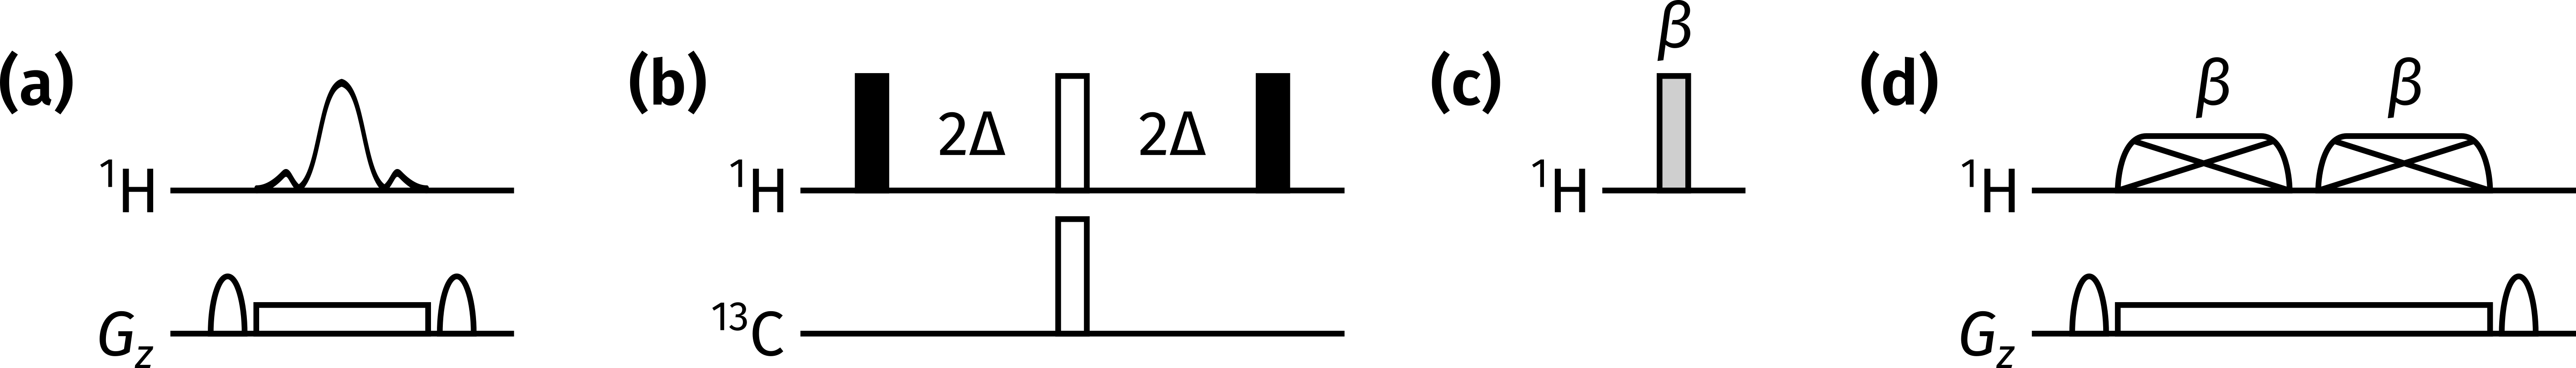
\includegraphics[]{pureshift/elements.png}
    {\phantomsubcaption\label{fig:pureshift_elements_zs}}
    {\phantomsubcaption\label{fig:pureshift_elements_bird}}
    {\phantomsubcaption\label{fig:pureshift_elements_tr}}
    {\phantomsubcaption\label{fig:pureshift_elements_psyche}}
    \caption[Pure shift elements]{
        A selection of pure shift elements.
        \textbf{(\subref{fig:pureshift_elements_zs})} Zangger--Sterk PSE\autocite{Zangger1997JMR}, involving the combination of a selective \ang{180} refocusing pulse and a weak gradient.
        \textbf{(\subref{fig:pureshift_elements_bird})} BIRD PSE\autocite{Garbow1982CPL,Aguilar2011ACIE}; the delay $\Delta$ is set to $1/(4 \cdot \oneJ{CH})$.
        \textbf{(\subref{fig:pureshift_elements_tr})} Time-reversal PSE\autocite{Sorensen1985JACS}, simply consisting of a hard pulse with variable flip angle $\beta$. Multiple spectra with different values of $\beta$ must be co-added to suppress artefacts (though not completely, as discussed in the text).
        \textbf{(\subref{fig:pureshift_elements_psyche})} PSYCHE PSE\autocite{Foroozandeh2014ACIE}, consisting of two saltire pulses\autocite{Foroozandeh2018CEJ,Foroozandeh2020JMR} with flip angle $\beta$, and a weak gradient.
    }
    \label{fig:pureshift_elements}
\end{figure}

We are finally now in a position to study individual PSEs and their mechanisms of action.
We begin with the Zangger--Sterk (ZS, or `slice-selective') PSE\autocite{Zangger1997JMR}, in which a selective refocusing pulse and a weak gradient are simultaneously applied (\cref{fig:pureshift_elements_zs}).
In practice, an rSNOB pulse\autocite{Kupce1995JMRSB} is often used as the refocusing pulse.
The effect of the gradient is to make each spin in the sample have a spatially dependent offset; therefore, in each \textit{slice} (or cross-section) of the sample, a different spin will fall within the specific bandwidth of the refocusing pulse.
This spin is refocused by the PSE and therefore becomes the active spin \textit{within that specific slice}; the bracketing pair of CTP gradients serve to destroy coherences on all the other spins which are not inverted.
Each signal of the pure shift spectrum therefore derives from a specific slice of the sample; during direct detection, all slices simultaneously contribute to the signal, thus yielding a broadband pure shift spectrum.

The sensitivity of the ZS method tends to be low (the factor $c$ tends to be on the order of $\sim 0.01$ to $0.05$), as each signal only comes from a narrow section of the sample.
Nevertheless, it still finds wide usage in pure shift applications nowadays, especially because it is compatible with the real-time acquisition mode\autocite{Meyer2013ACIE}: as long as the pulse and the weak gradient are the same each time, then the same active spins will always be chosen in the same slice (as long as diffusion effects are ignored).
The PSE can also be customised through the bandwidth of the refocusing pulse: decreasing this improves the spatial differentiation between spins which have similar intrinsic offsets, yielding better decoupling quality, albeit at the cost of sensitivity.
The ZS element can be easily---and has been---adapted for use in many experiments, including (but not limited to) absorption-mode 2DJ spectroscopy\autocite{Pell2007JMR} and selective refocusing (SERF) experiments for the measurement of $\nJ{HH}$\autocite{Giraud2010ACIE,Gubensak2014CC,Mishra2017JMR,Buchberger2018MRC}.

Next up is the \textit{bilinear rotation decoupling} (BIRD) pulse element (\cref{fig:pureshift_elements_bird}).
BIRD is not spatially selective like the ZS method; instead, it is \textit{isotope-selective} in that it acts as a $180^\circ_y$ pulse on \carbon{}--bound protons, and does not affect \carbont{}--bound protons.
Consequently, all \carbon{}--bound protons become the active spins in the context of pure shift NMR.
The first report of the BIRD element\autocite{Garbow1982CPL}, in 1982, was clearly ahead of its time: it reported the use of an interferogram-type approach to obtain 1D pure shift spectra.
However, in the subsequent decades, this seemed to have been forgotten: BIRD found much more use as an isotope-selective rotation element in heteronuclear NMR\autocite{Uhrin1993JMRSA}, until its use as a pure shift element was `rediscovered'\autocite{Sakhaii2009JMR,Aguilar2011ACIE}.

An immediate drawback of BIRD is that it does not decouple geminal (diastereotopic) \ch{CH2} groups, as both protons would be either both active or both passive.
The sensitivity penalty of BIRD is also relatively severe: the factor $c$ derives from the natural abundance of \carbon{}, which is approximately $0.011$.
However, it is also compatible with real-time acquisition\autocite{Lupulescu2012JMR}, and has found particular success as a pure shift element in the $F_2$ dimension of HMQC and HSQC experiments\autocite{Sakhaii2009JMR,Paudel2013ACIE,Reinsperger2014JMR,Kiraly2018MRC,Nolis2019JMR_psHSQC,Singh2020JMR}: in this case, the use of BIRD leads to no loss of sensitivity as only \carbon{}--bound protons are detected in HSQC experiments anyway.%
\footnote{In fact, the sensitivity is increased by the collapse of multiplet structure.}
It should be noted that the BIRD element does not need to be combined with a hard \ang{180} pulse to form a JRE: the inverse effect of only flipping the passive spins can be accomplished by simply changing the phase of both internal \ang{180} pulses to $+y$.
Using the nomenclature of Uhr{\'i}n et al.,\autocite{Uhrin1993JMRSA} the PSE and JRE forms of the BIRD pulse can be labelled as BIRD\textsuperscript{d,X} and BIRD\textsuperscript{r,X} respectively.

The \textit{time-reversal} PSE (\cref{fig:pureshift_elements_tr}) is even simpler: it consists only of one hard pulse with flip angle $\beta$\autocite{Sorensen1985JACS}.
The catch is that the experiment must be repeated with different values of $\beta$, and the results added up with specific weightings.\autocite{Griesinger1986JCP}
This leads to cancellation of \textit{some}, but not all, of the unwanted coherences: for example, on its own, it does not suppress COSY-type coherence transfer such as $I_{1-}I_{2\alpha} \to I_{1\alpha}I_{2+}$.
This proved to be inconsequential in the original application of $F_1$ decoupling in a 2D NOESY\autocite{Sorensen1985JACS}; however, it is not acceptable in a 1D context as it leads to substantial artefacts.
This will be discussed in more detail in \cref{sec:pureshift__timerev}, so a fuller analysis of the time-reversal PSE is deferred until then.

Finally, we come to the PSYCHE method, which is generally considered the current state of the art for pure shift NMR.\autocite{Foroozandeh2014ACIE}
The corresponding PSE (\cref{fig:pureshift_elements_psyche}) consists of two swept-frequency pulses applied during a weak gradient: for example, a pair of chirps with opposite sweep directions can be used.
Using two \textit{saltire pulses}, pulses which simultaneously sweep in both directions, leads to an increased signal-to-artefact ratio\autocite{Foroozandeh2018CEJ}.
The operation of this PSE is not easy to fully explain\autocite{Foroozandeh2020JMR}. However, we can adopt the (not fully accurate, but still useful) instant-flip approximation\autocite{Zwahlen1997JACS,Kupce2007JMR}---that the swept-frequency pulse acts as an instantaneous \ang{180} rotation on each frequency it passes through.
Using this, the PSYCHE element (or strictly, the PSYCHE JRE, including a hard \ang{180} pulse) may be viewed as a spatially parallelised version of the anti $z$-COSY experiment\autocite{Oschkinat1986JMR,Pell2007MRC}, which we now describe.

\subsection{PSYCHE in detail}
\label{subsec:pureshift__psyche_analysis}

\begin{figure}[ht]
    \centering
    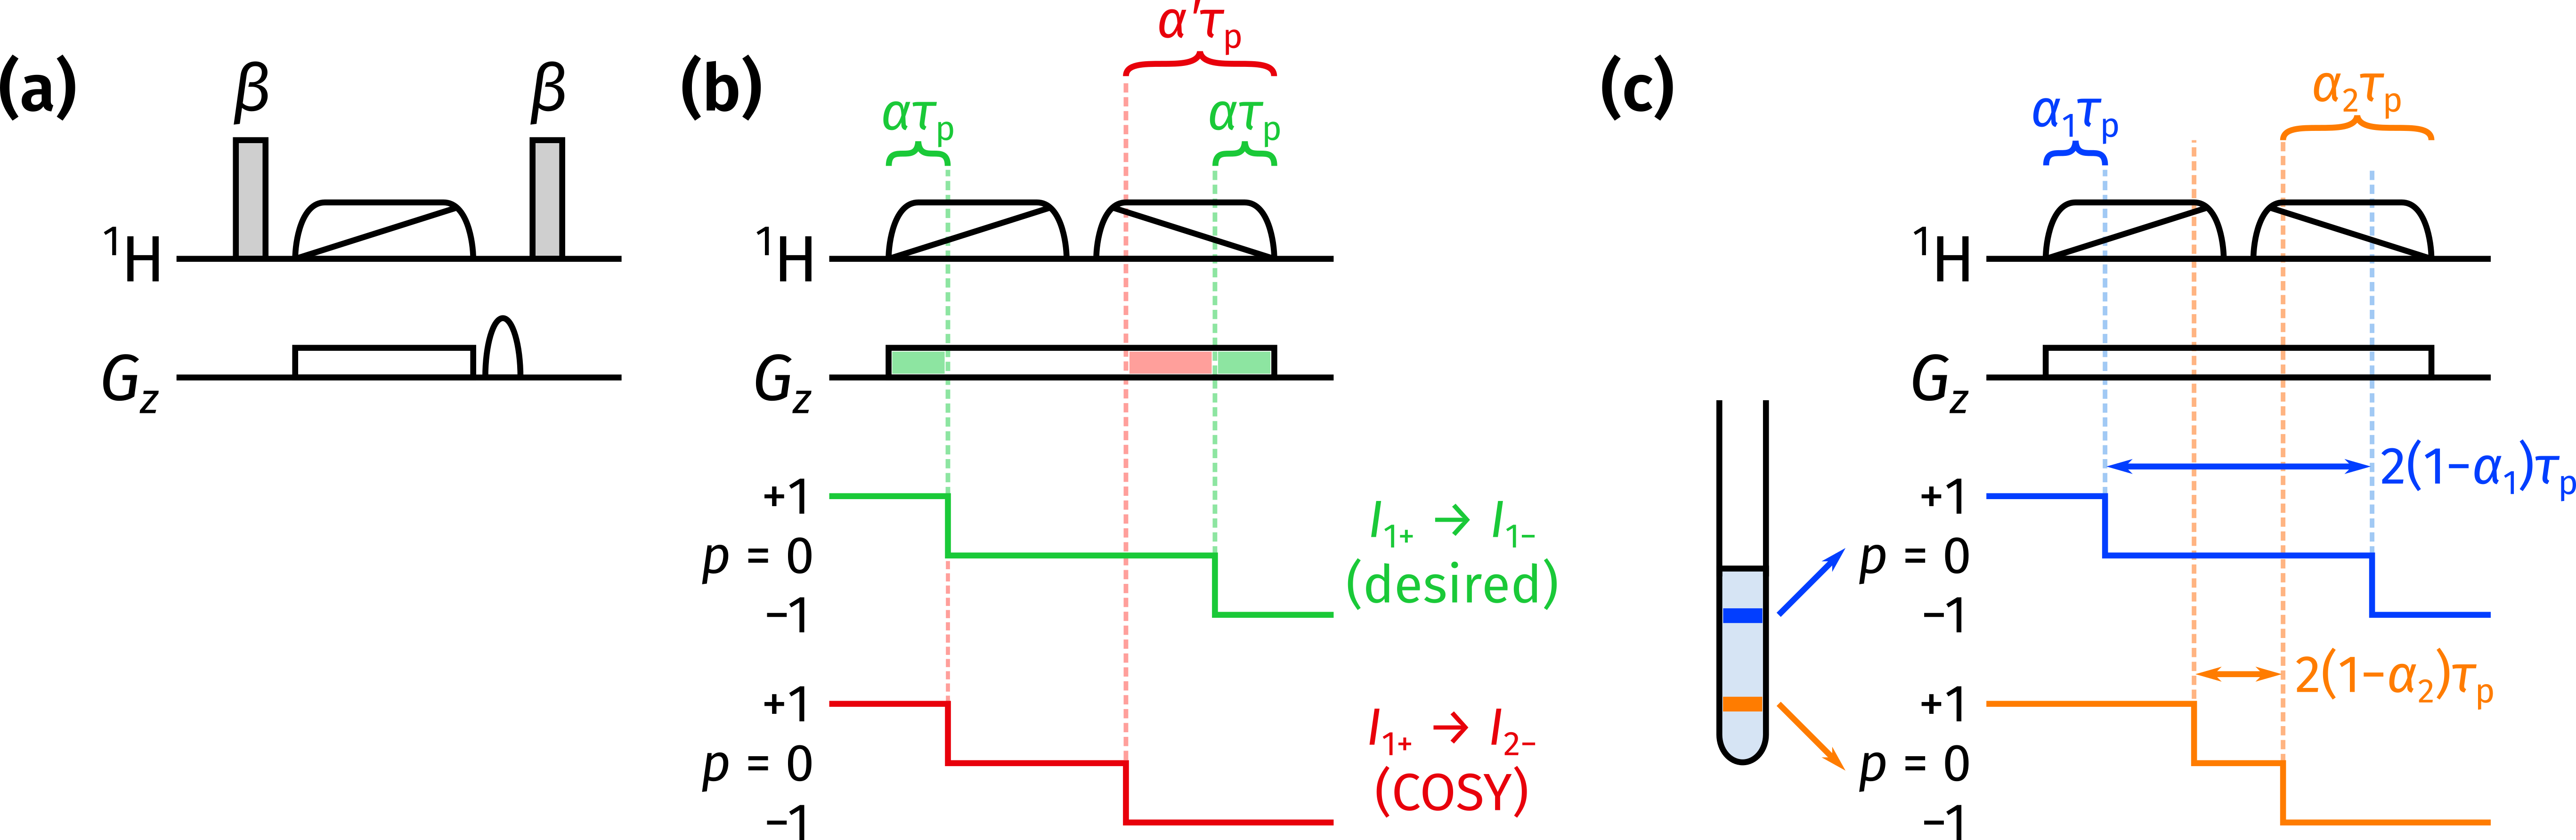
\includegraphics[]{pureshift/psyche_detail.png}%
    {\phantomsubcaption\label{fig:psyche_detail_antizcosy}}%
    {\phantomsubcaption\label{fig:psyche_detail_cosy_suppress}}%
    {\phantomsubcaption\label{fig:psyche_detail_zqc_suppress}}%
    \caption[Detailed analysis of anti $z$-COSY and PSYCHE]{
        A closer look at the mechanism of the PSYCHE PSE.
        \textbf{(\subref*{fig:psyche_detail_antizcosy})} The $\beta$--$z$-filter--$\beta$ mixing period used in the original anti $z$-COSY experiment. This has a similar action to a JRE, but does not suppress COSY-type coherence transfers from spin $i$ to spin $j$.
        \textbf{(\subref*{fig:psyche_detail_cosy_suppress})} An illustration of how COSY-type artefacts are suppressed by the PSYCHE pulse element. The desired CTP which remains on spin 1 is rephased by the gradients, but the COSY CTP is dephased.
        \textbf{(\subref*{fig:psyche_detail_zqc_suppress})} An illustration of how zero-quantum terms are suppressed by the PSYCHE element through spatial averaging: in each slice of the sample (highlighted in blue and orange), the zero-quantum terms are allowed to evolve for a different duration.
    }
    \label{fig:psyche_detail}
\end{figure}

The anti $z$-COSY experiment utilises a $\beta$--$z$-filter--$\beta$ mixing period (\cref{fig:psyche_detail_antizcosy}), where $\beta$ is a small angle, typically \ang{10} to \ang{20}.
The role of the $z$-filter\autocite{Thrippleton2003ACIE} is to remove zero-quantum terms such as $I_{1-}I_{2+}$ between the two $\beta$ pulses, retaining only population terms such as $I_{1\alpha}I_{2\alpha}$.
The CTPs which this mixing period selects for ultimately give rise to peaks which lie perpendicular to the main diagonal of the spectrum.
In an elegant paper, Pell et al.\autocite{Pell2007MRC} showed that by isolating the diagonal peaks of a 2D anti $z$-COSY experiment and taking the \ang{45} projection of these, a pure shift spectrum could be obtained.
Here, we will go one step further and consider the \textit{direct} use of this element as a JRE: this will reveal some problems which are neatly taken care of by the PSYCHE experiment.

We first need to introduce how the basis operators $\{I_+, I_-, I_\alpha, I_\beta\}$ evolve under a hard pulse (applied along the $x$-axis) with flip angle $\beta$:
\begin{align}
    I_{\pm} &\xrightarrow{\beta I_x} c^2 I_{\pm} + s^2I_{\mp} \pm \frac{\mi S}{2}(I_\alpha - I_\beta) \label{eq:ipm_beta_evolution} \\
    I_{\alpha} &\xrightarrow{\beta I_x} c^2 I_{\alpha} + s^2I_{\beta} + \frac{\mi S}{2}(I_+ - I_-) \label{eq:ialpha_beta_evolution} \\
    I_{\beta} &\xrightarrow{\beta I_x} c^2 I_{\beta} + s^2I_{\alpha} - \frac{\mi S}{2}(I_+ - I_-) \label{eq:ibeta_beta_evolution}
\end{align}
where $S = \sin\beta$, $s = \sin(\beta/2)$, and $c = \cos(\beta/2)$.
Using these formulae, we can show that for a two-spin system (see Pell et al.\autocite{Pell2007MRC} for the equivalent analysis on a three-spin system), the $\beta$--$z$-filter--$\beta$ element converts the term $I_{1+}I_{2\alpha}$ to
\begin{equation}
    \label{eq:anti_z_cosy_transitions}
    I_{1+}I_{2\alpha} \longrightarrow
    {\underbrace{\frac{1}{2}S^2c^4 I_{1+}I_{2\beta}}_\text{term 1}}
    + {\underbrace{S^2c^2s^2I_{1+}I_{2\alpha}}_{\text{term 2}}}
    - {\underbrace{\frac{1}{4}S^2c^4I_{1\alpha}I_{2+}
    + \frac{1}{4}S^2c^4I_{1\beta}I_{2+}}_{\text{terms 3 and 4}}}
    + \cdots,
\end{equation}
where other terms with different coherence orders have been neglected (on the basis that they can be easily suppressed with bracketing CTP gradients), and terms with higher orders in $s$ have been discarded since $s = \sin(\beta/2) \ll 1$ for small $\beta$.

The first term $I_{1+}I_{2\beta}$, corresponding to the flipping of passive spins only, is the only term we want to see from a JRE.
The second term, $I_{1+}I_{2\alpha}$, corresponds to the case where neither active nor passive spins have been flipped.
In the original anti $z$-COSY work, these give rise to `off-diagonal' peaks which are part of a multiplet on the diagonal, but when projected at \ang{45} generate artefacts around the pure shift peak.
In the context of pure shift NMR, these are called `recoupling artefacts', as they arise from imperfect J-refocusing.
Note that the ratio of recoupling artefacts to desired signal is proportional to $S^2c^2s^2/S^2c^4 = \tan^2(\beta/2)$: using a smaller value for $\beta$ therefore leads to better signal-to-artefact ratios, but also lower overall sensitivity.
The PSYCHE element is similar to the $\beta$--$z$-filter--$\beta$ element in this regard: it does not suppress the recoupling artefacts, but instead relies on the user choosing a suitable value for $\beta$ such that the artefact-to-signal ratio is tolerably small.
If the sensitivity proves to be insufficient, the flip angle $\beta$ may be increased instead: this leads to a larger artefact-to-signal ratio, but if the sample is not concentrated anyway, it may well be that the artefacts do not rise above the noise level.%

The third and fourth terms, $I_{1\lambda}I_{2+}$ ($\lambda \in \{\alpha,\beta\}$), represent `COSY-type' coherence transfer to a coupled spin.
In the original anti $z$-COSY, these led to crosspeak multiplets at $(\Omega_1, \Omega_2)$, which could be removed by hand before taking the projection.
However, in a pure shift sequence, the peaks arising from these terms cannot simply be removed in the same way.
It is precisely this issue which precludes the $\beta$--$z$-filter--$\beta$ element from being directly used as a JRE, and motivates the development of the PSYCHE PSE, which \textit{does} suppress these coherence transfers.

To understand how this occurs, we invoke the instantaneous spin-flip assumption.
Each coherence $I_{i+}$ is converted (or `flipped') to a population term $I_{1\lambda}$ at a specific point $\alpha\taup$ after the start of the first chirp, and can be reconverted to a coherence on the same spin $I_{i-}$ at a time $\alpha\taup$ before the end of the second chirp (the blue CTP in \cref{fig:psyche_detail_cosy_suppress}).%
\footnote{Note the change in the sign of the coherence, which differs from the analysis of the anti $z$-COSY experiment. This arises because we are only considering the PSYCHE PSE on its own, \textit{not} the JRE.}
Here, $\taup$ is the duration of the chirp, and $0 < \alpha < 1$.
In this case, the coherence is perfectly rephased by the weak gradient applied during the chirp pulses, since the \textit{time} it experiences these gradients for is the same on both sides of the chirps.
Now, if the $I_{i+}$ term is instead converted to a coherence on a different spin $I_{j-}$, it experiences the gradient for a total duration of $\alpha\taup$ after the start of the first chirp, and also $\alpha'\taup$ before the end of the second chirp (the orange CTP in \cref{fig:psyche_detail_cosy_suppress}).
In general, $\alpha \neq \alpha'$ as spins $i$ and $j$ have different offsets; therefore, this CTP is dephased by the gradients, resulting in suppression of the COSY-type artefacts in the spectrum.

It remains to also consider how the PSYCHE element selects for the population terms between the two spin flips.
Any terms with nonzero coherence order are of course simply dephased by the weak gradient.
However, zero-quantum terms (in homonuclear systems) are not dephased by gradients, and to eliminate them in a single-scan manner, they must be spatially averaged, for example by a $z$-filter.
It turns out that the PSYCHE element also results in a similar spatial averaging.
Following on from the previous paragraph, the time \textit{between} the spin flips (for the desired pathways, i.e.\ not COSY-type coherence transfer) is given by $2(1 - \alpha)\taup$.
At the same time, the weak gradient induces a range of offsets across the sample, much like in the Zangger--Sterk experiment.
Thus, the offset, and thus the value of $\alpha$, for a given spin depends on which slice it is in; for example, \cref{fig:psyche_detail_zqc_suppress} uses values of $\alpha_1$ and $\alpha_2$ for two different slices (blue and orange).
If zero-quantum terms are present between the spin flips, they evolve during this time and accrue a spatially-dependent phase: summation of these during FID acquisition leads to a cancellation of these terms.
Only population terms such as $I_{1\alpha}I_{2\alpha}$ survive during this, as they do not precess during this time.

The sensitivity of PSYCHE is significantly better than for other methods: depending on the flip angle $\beta$ chosen, $c$ is typically on the order of $0.05$--$0.15$ (see also \cref{fig:fa_dependence_124} for explicit simulations).
Furthermore, it is generally more robust with respect to strong coupling compared to other pure shift methods (artefacts from strong coupling often arise due to unexpected coherence transfer\autocite{Thrippleton2005JMR}, which is suppressed in a similar way to the COSY-type artefacts).
These two factors alone have meant that PSYCHE has enjoyed substantial adoption since its introduction: a large number of 2D experiments utilising PSYCHE decoupling in either $F_1$ or $F_2$ have been developed,\autocite{Foroozandeh2014JACS,Timari2015CEJ,Koos2016ACIE,Sinnaeve2016ACIE,Aguilar2018MRC,Kaltschnee2016JMR,Ilgen2021JMR} notably the PSYCHE-iDOSY diffusion experiment\autocite{Foroozandeh2016ACIE}, where the increased resolution provided by pure shift spectroscopy translates into increased resolution in the \textit{diffusion} dimension as well.
Like the ZS element before it, the PSYCHE element has also been used for the acquisition of absorption-mode 2DJ spectra.\autocite{Foroozandeh2015CC}

Despite this success, PSYCHE suffers from one significant drawback: it cannot be used in a real-time fashion.
The PSYCHE PSE is often said to select active and passive spins in a `statistical' manner: this is because of the $c^2$ and $s^2$ terms arising from the low-flip angle pulses.
What this really means is that we do not care \textit{exactly} which spins are active and which are passive, but that a certain proportion of the spins are active and passive.
Repeated application of the PSE therefore does not select for the same active spins each time, which precludes its application to real-time acquisition.

Although the PSYCHE PSE may appear deceptively simple at first glance, the closer analysis given here (and elsewhere\autocite{Foroozandeh2018CEJ}) clearly shows that its inner workings are anything but.
Along with other ingenious experiments such as the $z$-filter\autocite{Thrippleton2005JMR}, ultrafast NMR\autocite{Frydman2002PNASUSA,Pelupessy2003JACS,Frydman2003JACS}, and more recently GEMSTONE\autocite{Kiraly2021ACIE}, PSYCHE is a prime example of how \textit{spatiotemporal averaging} and pulsed field gradients can be used to great effect in modern NMR spectroscopy.\autocite{Dumez2018PNMRS}

At the same time, PSYCHE itself is not \textit{perfect}: it does not fully suppress recoupling artefacts, and can only be used in the interferogram mode.
To improve on PSYCHE would therefore entail one of the following:
\begin{enumerate}
    \item increasing the sensitivity (while maintaining purity);
    \item increasing the purity (while maintaining sensitivity); or
    \item developing a pure shift element which is compatible with real-time acquisition while giving comparable sensitivity and purity to PSYCHE.
\end{enumerate}

The sections which follow describe my efforts towards objectives (1) and (2).


\section{PSYCHE with a variable number of saltires}
\label{sec:pureshift__nsaltire}

\begin{figure}[htb]
    \centering
    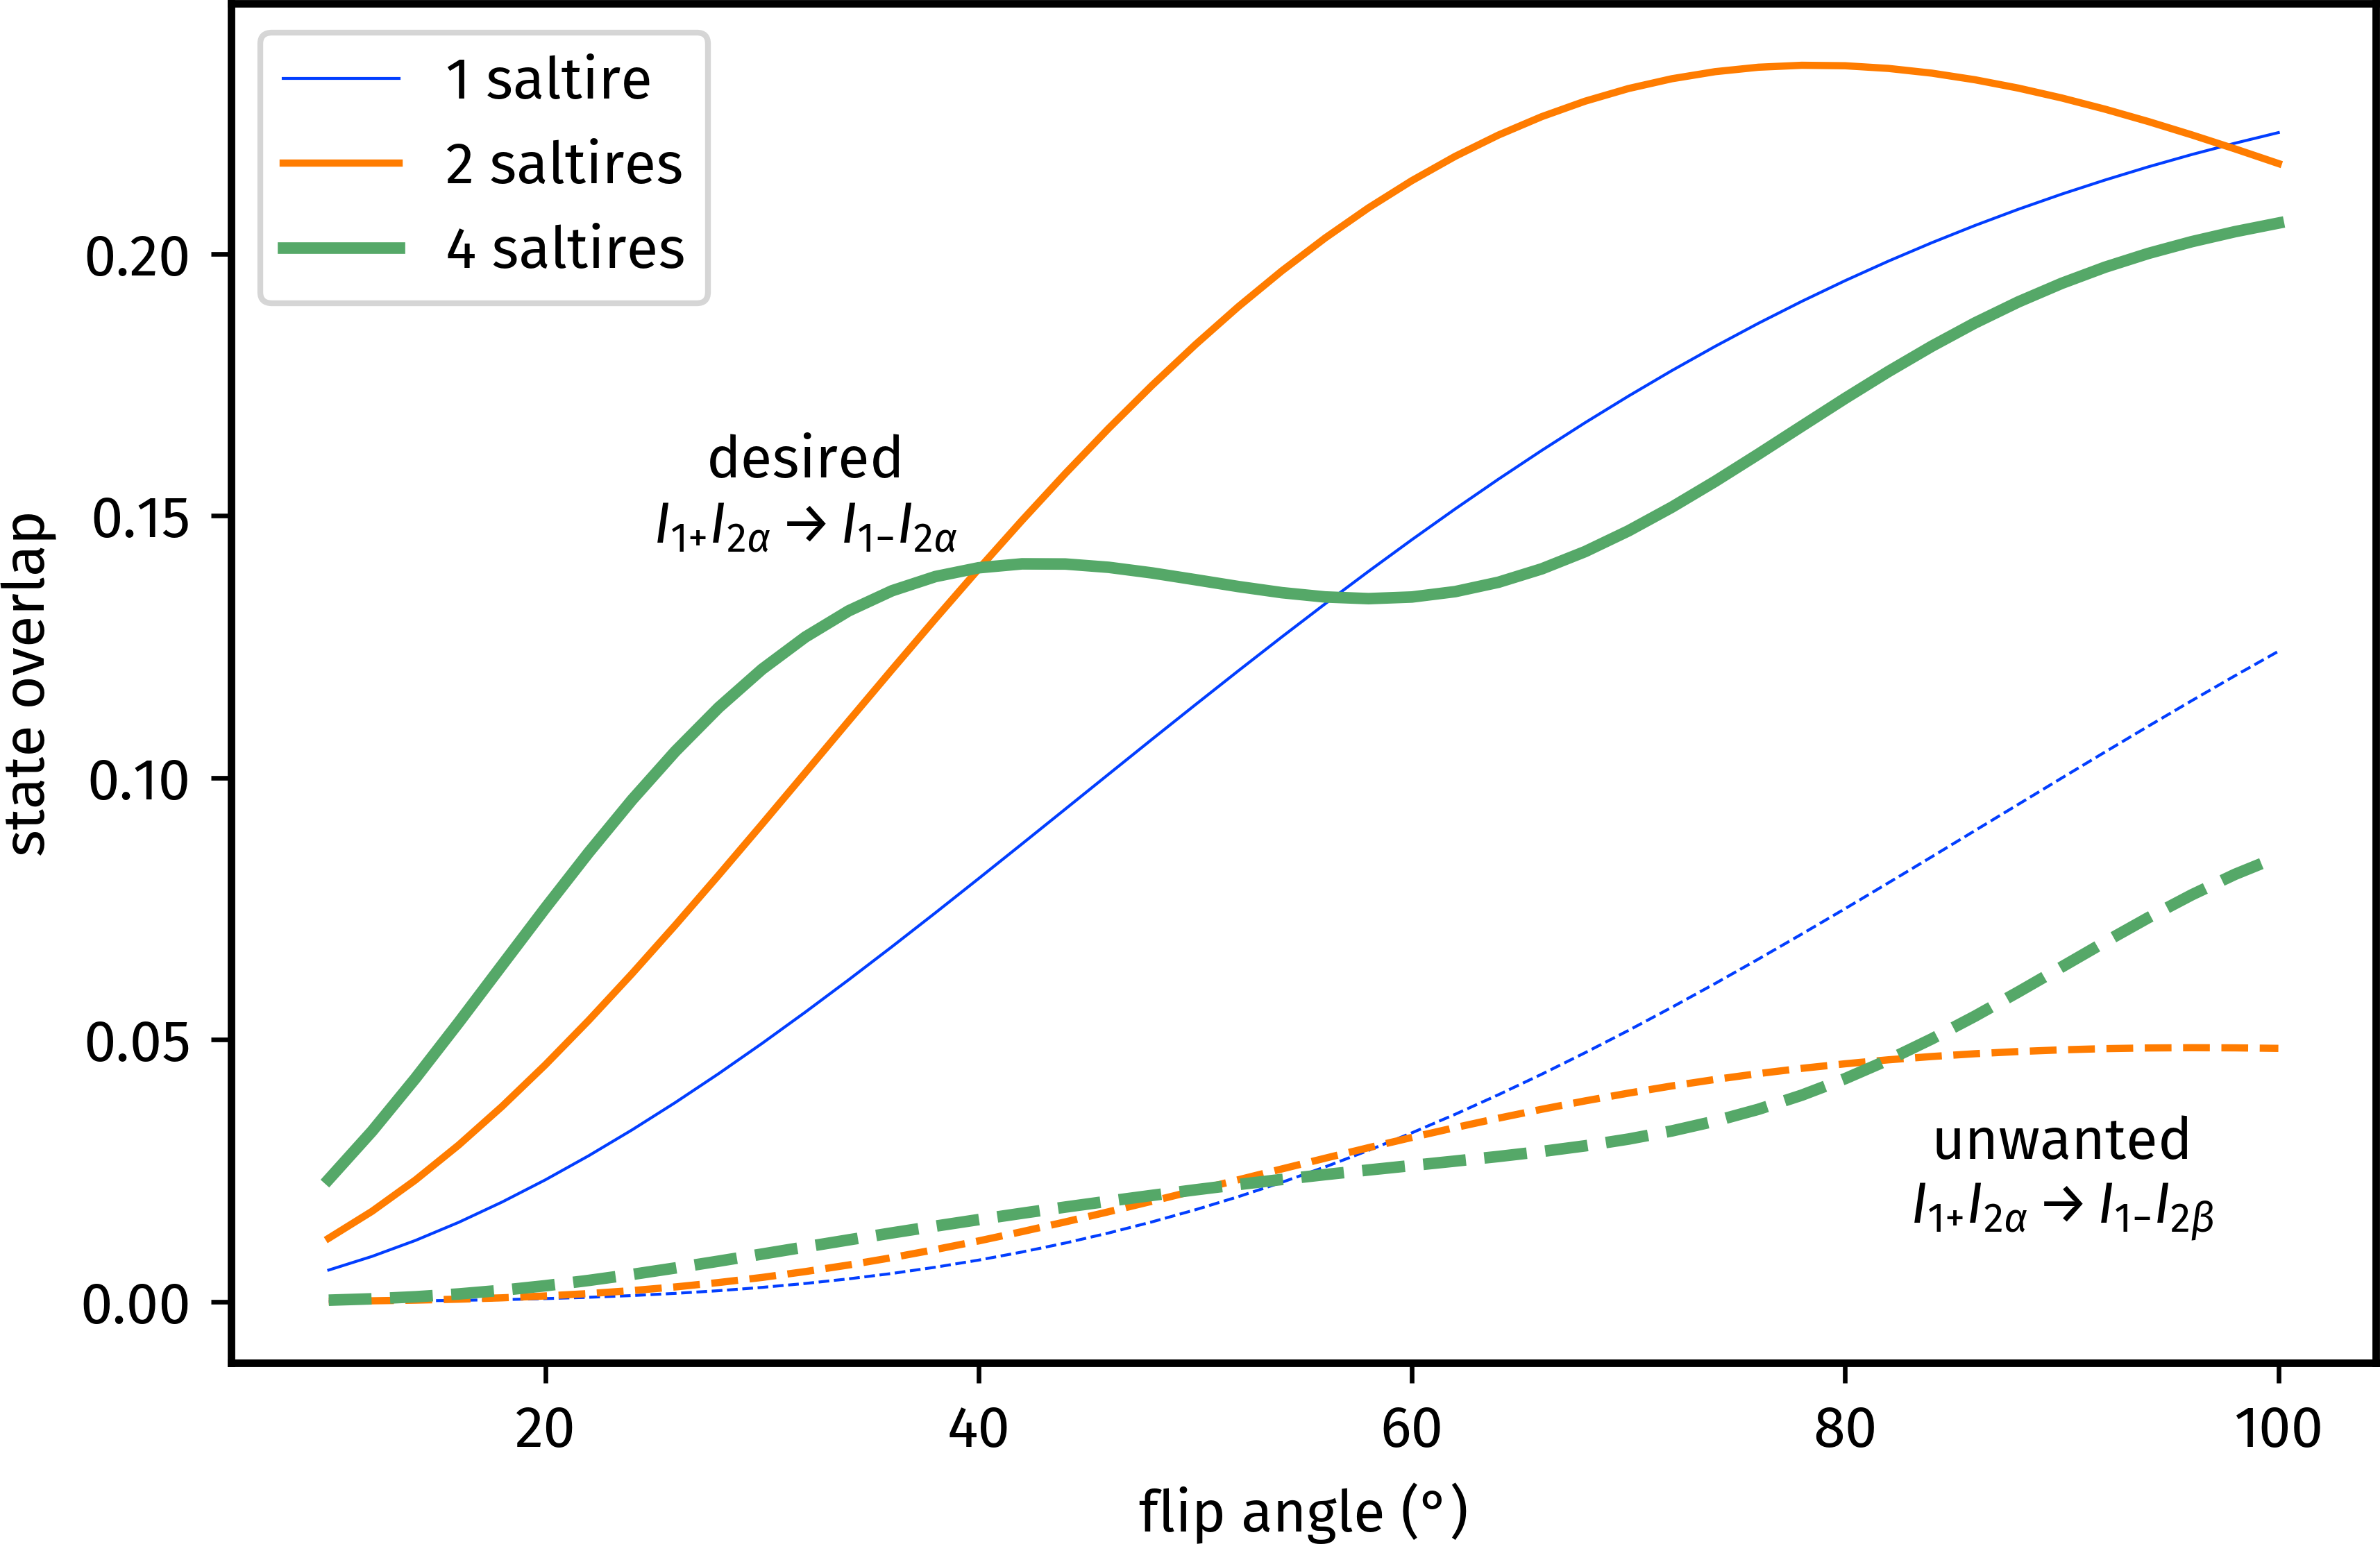
\includegraphics[]{pureshift/fa_dependence_124.png}%
    \caption[Signal and artefact intensity with 1-, 2-, and 4-saltire PSYCHE]{Simulated signal and artefact intensity for various PSYCHE-style PSEs as a function of the flip angle used.
    Calculations were performed on a two-spin system with a coupling of \SI{7}{\Hz}, and an offset difference of \SI{1.5}{\kHz}.
    The total PSE duration was \SI{30}{\ms} (so, for example, in the four-saltire PSYCHE, each saltire was \SI{7.5}{\ms}).
    Solid lines indicate the coefficients for the desired $I_{1+}I_{2\alpha} \to I_{1-}I_{2\alpha}$ pathway which contributes to the pure shift signal; dashed lines the coefficients for the undesired $I_{1+}I_{2\alpha} \to I_{1-}I_{2\beta}$ pathway, which gives rise to recoupling artefacts.
}
    \label{fig:fa_dependence_124}
\end{figure}

The first attempted method was to change the number of saltire pulses used in the PSYCHE PSE.
As described in \cref{subsec:pureshift__psyche_analysis}, PSYCHE relies on spatiotemporal averaging to suppress unwanted artefacts: this crucially relies on the fact that the pulse(s) used in the PSE are symmetric.
This can be accomplished with two opposing chirps, or two saltires, both of which are symmetric.
However, a \textit{single} saltire is also symmetric in itself: it is not hard to show that a single saltire can provide the requisite averaging.
Likewise, the use of four saltires would also be valid.

Theoretical simulations show that the overall profile of signal and artefact versus flip angle varies with the number of saltires (\cref{fig:fa_dependence_124}).
Generally, using a larger number of saltires but with a smaller flip angle accomplishes a similar sensitivity level.
This may be qualitatively rationalised as more saltires providing more possible CTPs which generate the desired signal (the same idea is generally invoked when discussing the difference between unidirectional chirps and saltires\autocite{Foroozandeh2018CEJ}).
However, regardless of the number of saltires, the fundamental strategy of adjusting the flip angle to control the signal-to-artefact ratio remains valid, which naturally raises the question of whether specific waveforms and flip angles can be chosen in order to obtain the best decoupling quality.

\begin{figure}[htb]
    \centering
    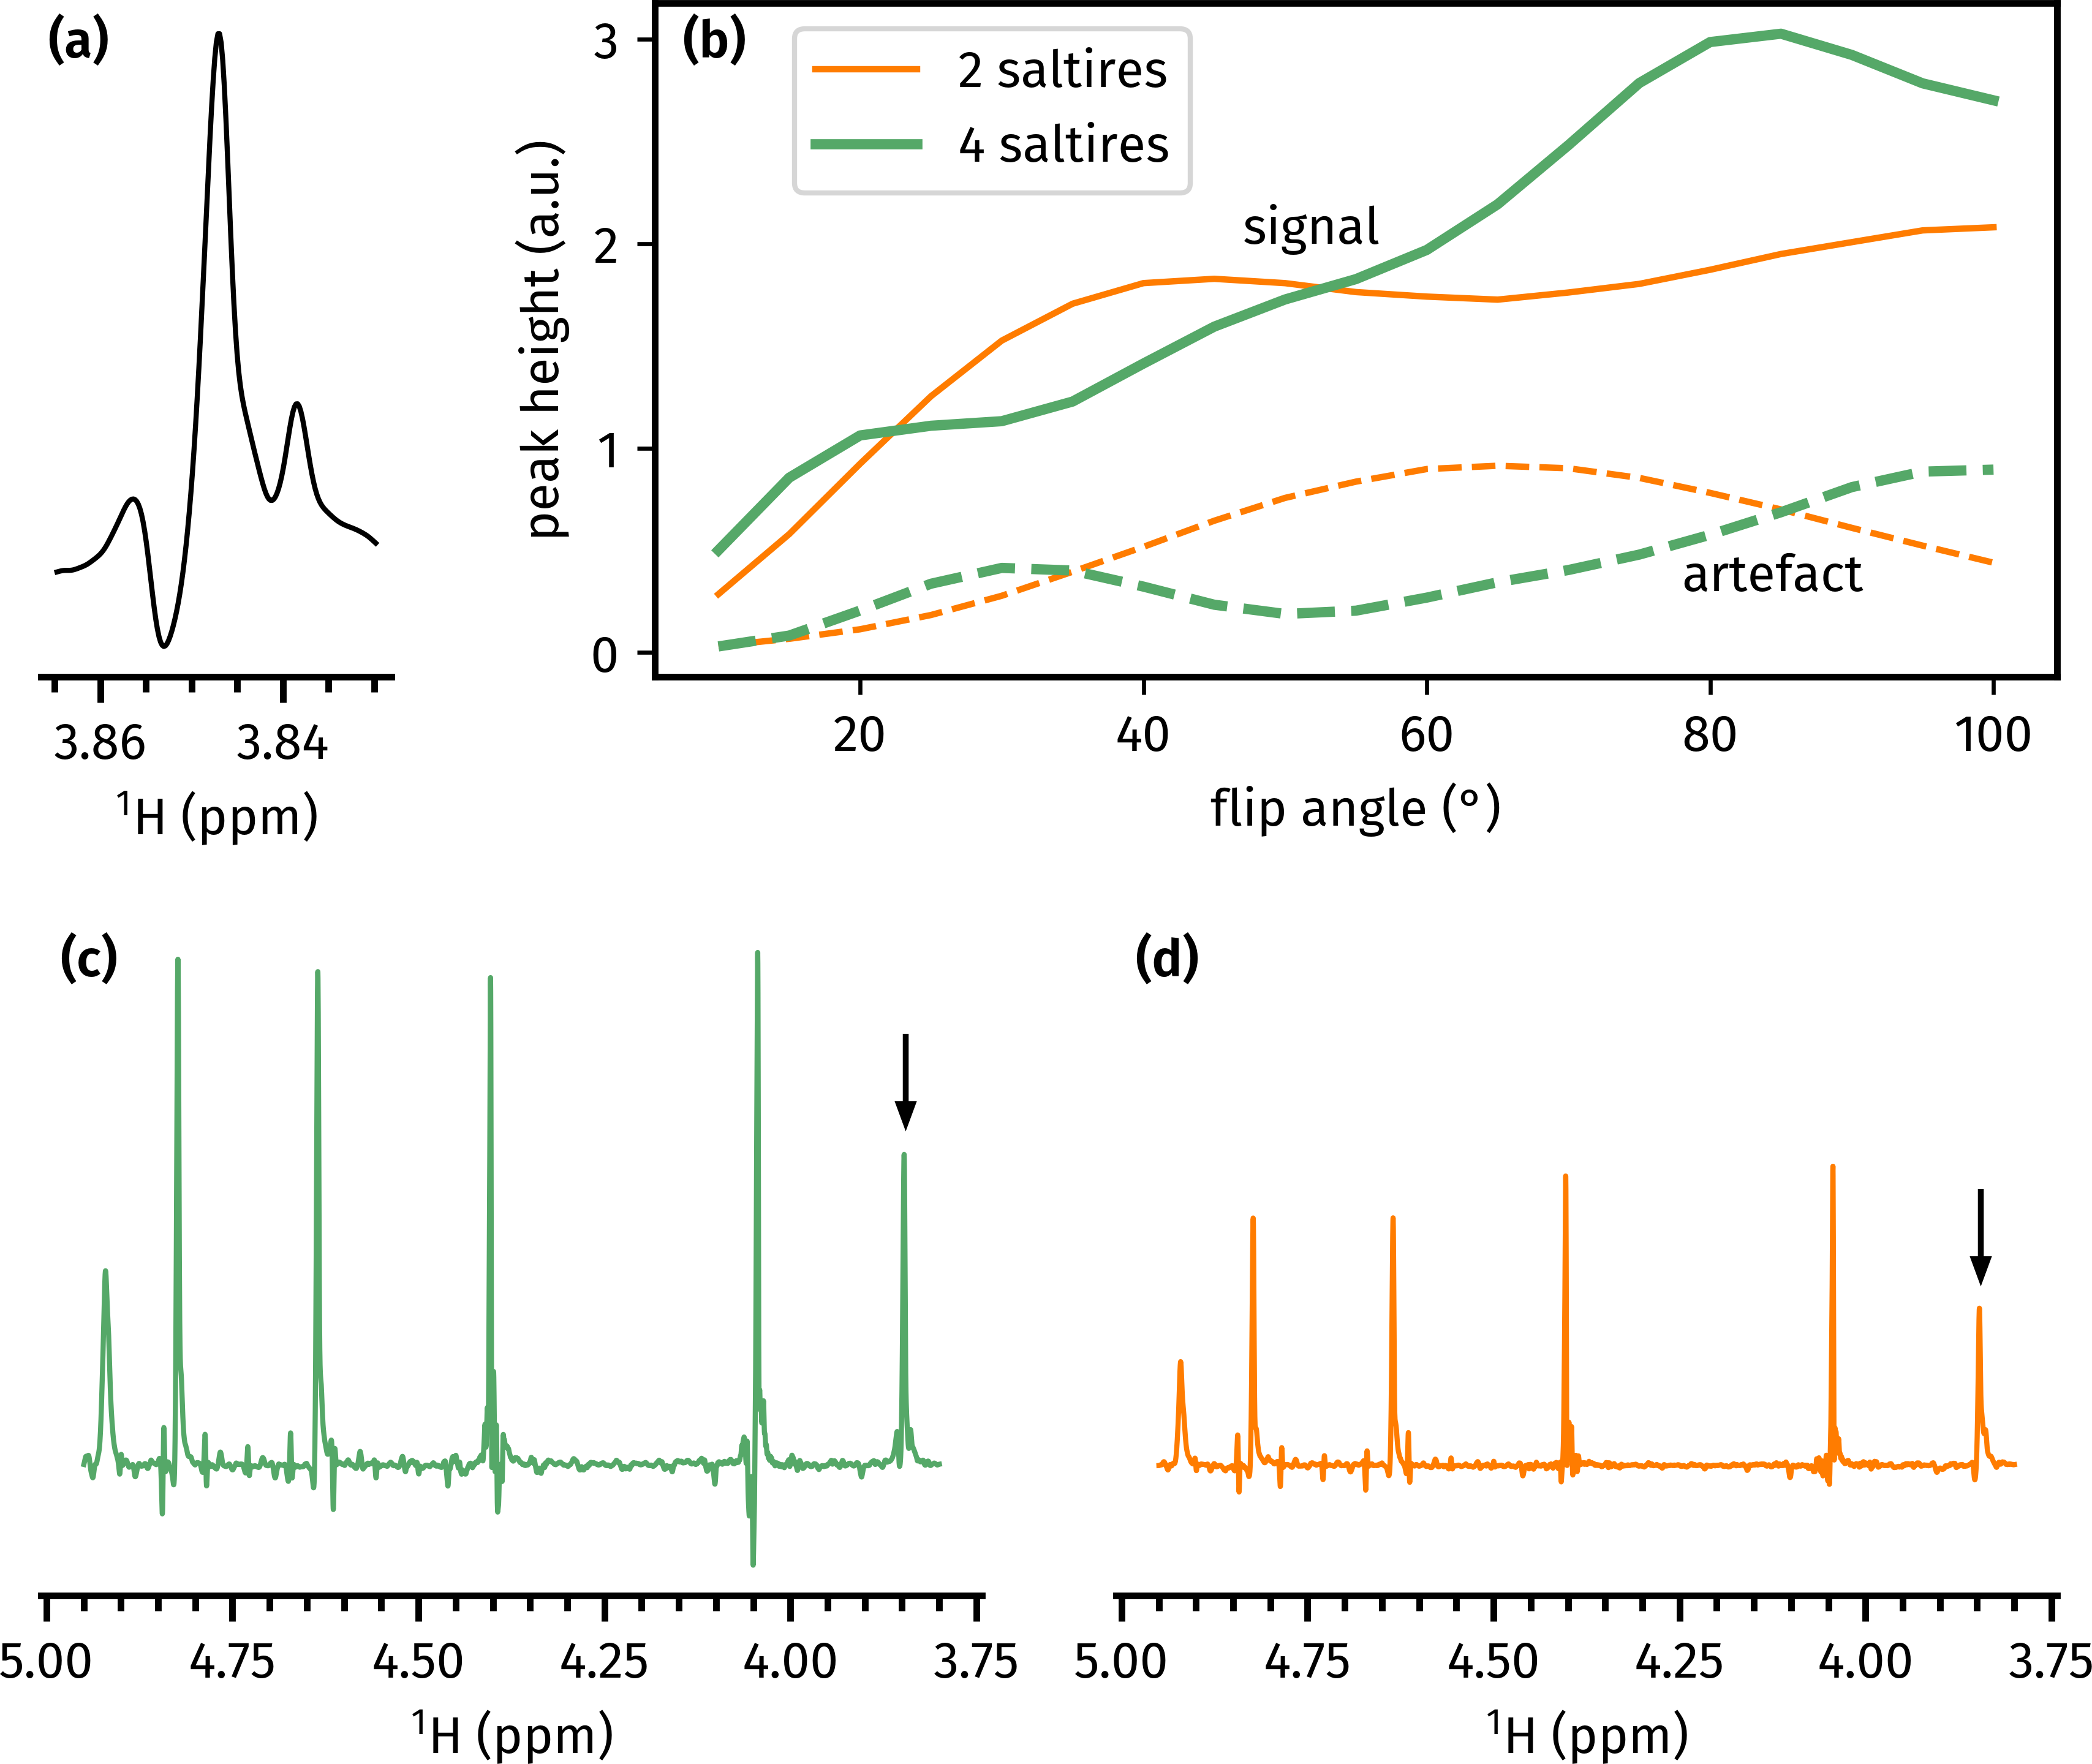
\includegraphics[]{pureshift/quadruple_saltire_30ms.png}%
    {\phantomsubcaption\label{fig:quadruple_saltire_30ms_spec}}%
    {\phantomsubcaption\label{fig:quadruple_saltire_30ms_plot}}%
    {\phantomsubcaption\label{fig:quadruple_saltire_30ms_maybebetter}}%
    {\phantomsubcaption\label{fig:quadruple_saltire_30ms_reference}}%
    \caption[Comparison of 30 ms double saltire and 30 ms quadruple saltire]{
        \textbf{(\subref{fig:quadruple_saltire_30ms_spec})} The peak in the pure shift spectrum of andrographolide used for calculation of signal and artefact intensity.
        The recoupling artefacts flanking the main peak are clearly visible.
        \textbf{(\subref{fig:quadruple_saltire_30ms_plot})} Peak heights of the desired signal (the central peak, solid lines) and artefacts (the mean of the two flanking peaks, dashed lines), as a function of flip angle.
        \textbf{(\subref{fig:quadruple_saltire_30ms_maybebetter})} Quadruple-saltire PSYCHE with $\beta = 55^\circ$.
        \textbf{(\subref{fig:quadruple_saltire_30ms_reference})} The reference spectrum, a double-saltire PSYCHE with $\beta = 20^\circ$.
        The peak at \SI{3.85}{ppm} used for the sensitivity and purity analysis is labelled with an arrow.
        \datacode{7A-201016}
    }
    \label{fig:quadruple_saltire_30ms}
\end{figure}

The quadruple-saltire PSYCHE was first evaluated experimentally.
In the first instance, I set the total duration of the PSE to \SI{30}{\ms}, meaning that each saltire was \SI{7.5}{\ms} long.
In this experiment, the sensitivity was defined as the maximum height of the main peak in \cref{fig:quadruple_saltire_30ms_spec}, and the artefact as the mean of the maximum heights of the two artefacts surrounding it.
The plot in \cref{fig:quadruple_saltire_30ms_plot} shows how these quantities vary as a function of the flip angle.
Interestingly, for the artefacts, the profile observed is similar to that in the simulations: the double-saltire version performs better at low and very high flip angles, but in the middle there is a region where the quadruple-saltire version has lower artefact intensity.
The signal intensities for both the double- and quadruple-saltire versions, however, seem to plateau off rather more quickly than the simulations suggest.

To highlight one particular data point, \cref{fig:quadruple_saltire_30ms_plot} suggests that the quadruple-saltire experiment with $\beta \approx 55^\circ$ has a similar artefact level to the double-saltire experiment with $\beta \approx 20^\circ$, but with substantially greater signal intensity.
Insets from these two spectra are respectively shown in \cref{fig:quadruple_saltire_30ms_maybebetter,fig:quadruple_saltire_30ms_reference}.
This conclusion does indeed seem to be true for the specific peak used for this analysis, which is at the right edge of the spectral insets shown here.
Overall, the quadruple-saltire \ang{55} experiment does have better sensitivity than the double-saltire \ang{20} experiment.
However, the artefacts are not always suppressed as nicely as in the chosen reference peak: for example, the peak at \SI{4.05}{ppm} is significantly less clean in the quadruple-saltire experiment.
Any apparent advantage over the double-saltire experiment is therefore not very clear---at least from this data alone.%
\footnote{In fact, I also performed some preliminary experiments where the four-saltire PSE was lengthened to \SI{60}{\ms}. The artefact behaviour in these spectra were better than in their \SI{30}{\ms} counterparts, which is to be expected since a longer PSE leads to better spatiotemporal averaging. However, I unfortunately did not compare these against a \SI{60}{\ms} double-saltire experiment, so these results are not included in this thesis. (It would be rather unfair to compare them against the \SI{30}{\ms} double-saltire.)}

Moving on to the single-saltire case, in addition to searching for a better signal and artefact profile as before, another possible motivation would be that the duration of the PSE can be decreased.
This would minimise losses due to relaxation and diffusion during the PSE, which were not taken into account in \cref{fig:fa_dependence_124} (and the simulations there did not vary $\taup$ anyway).
A single-saltire PSYCHE experiment was thus recorded with various combinations of flip angle ($\beta/^\circ \in \{15, 20, 25, 28, 30\}$) and pulse duration ($\taup/\text{ms} \in \{15, 25, 30, 35, 45, 55\}$).
In a similar way to the quadruple-saltire study, the sensitivity was defined as the maximum height of the main peak in \cref{fig:single_saltire_results_spec},%
\footnote{As an alternative, the Bruker \texttt{sinocal} AU programme was also used to measure the sensitivity of the spectrum; it yielded extremely similar results, so is not shown here. I found the \texttt{sinocal} routine to be rather unreproducible as the exact value calculated depends on random noise.}
and the artefact as the mean of the heights of the two artefacts surrounding it.
(However, note that the sample used was different.)
The purity, or signal-to-artefact ratio, is simply the former divided by the latter.

\begin{figure}[htb]
    \centering
    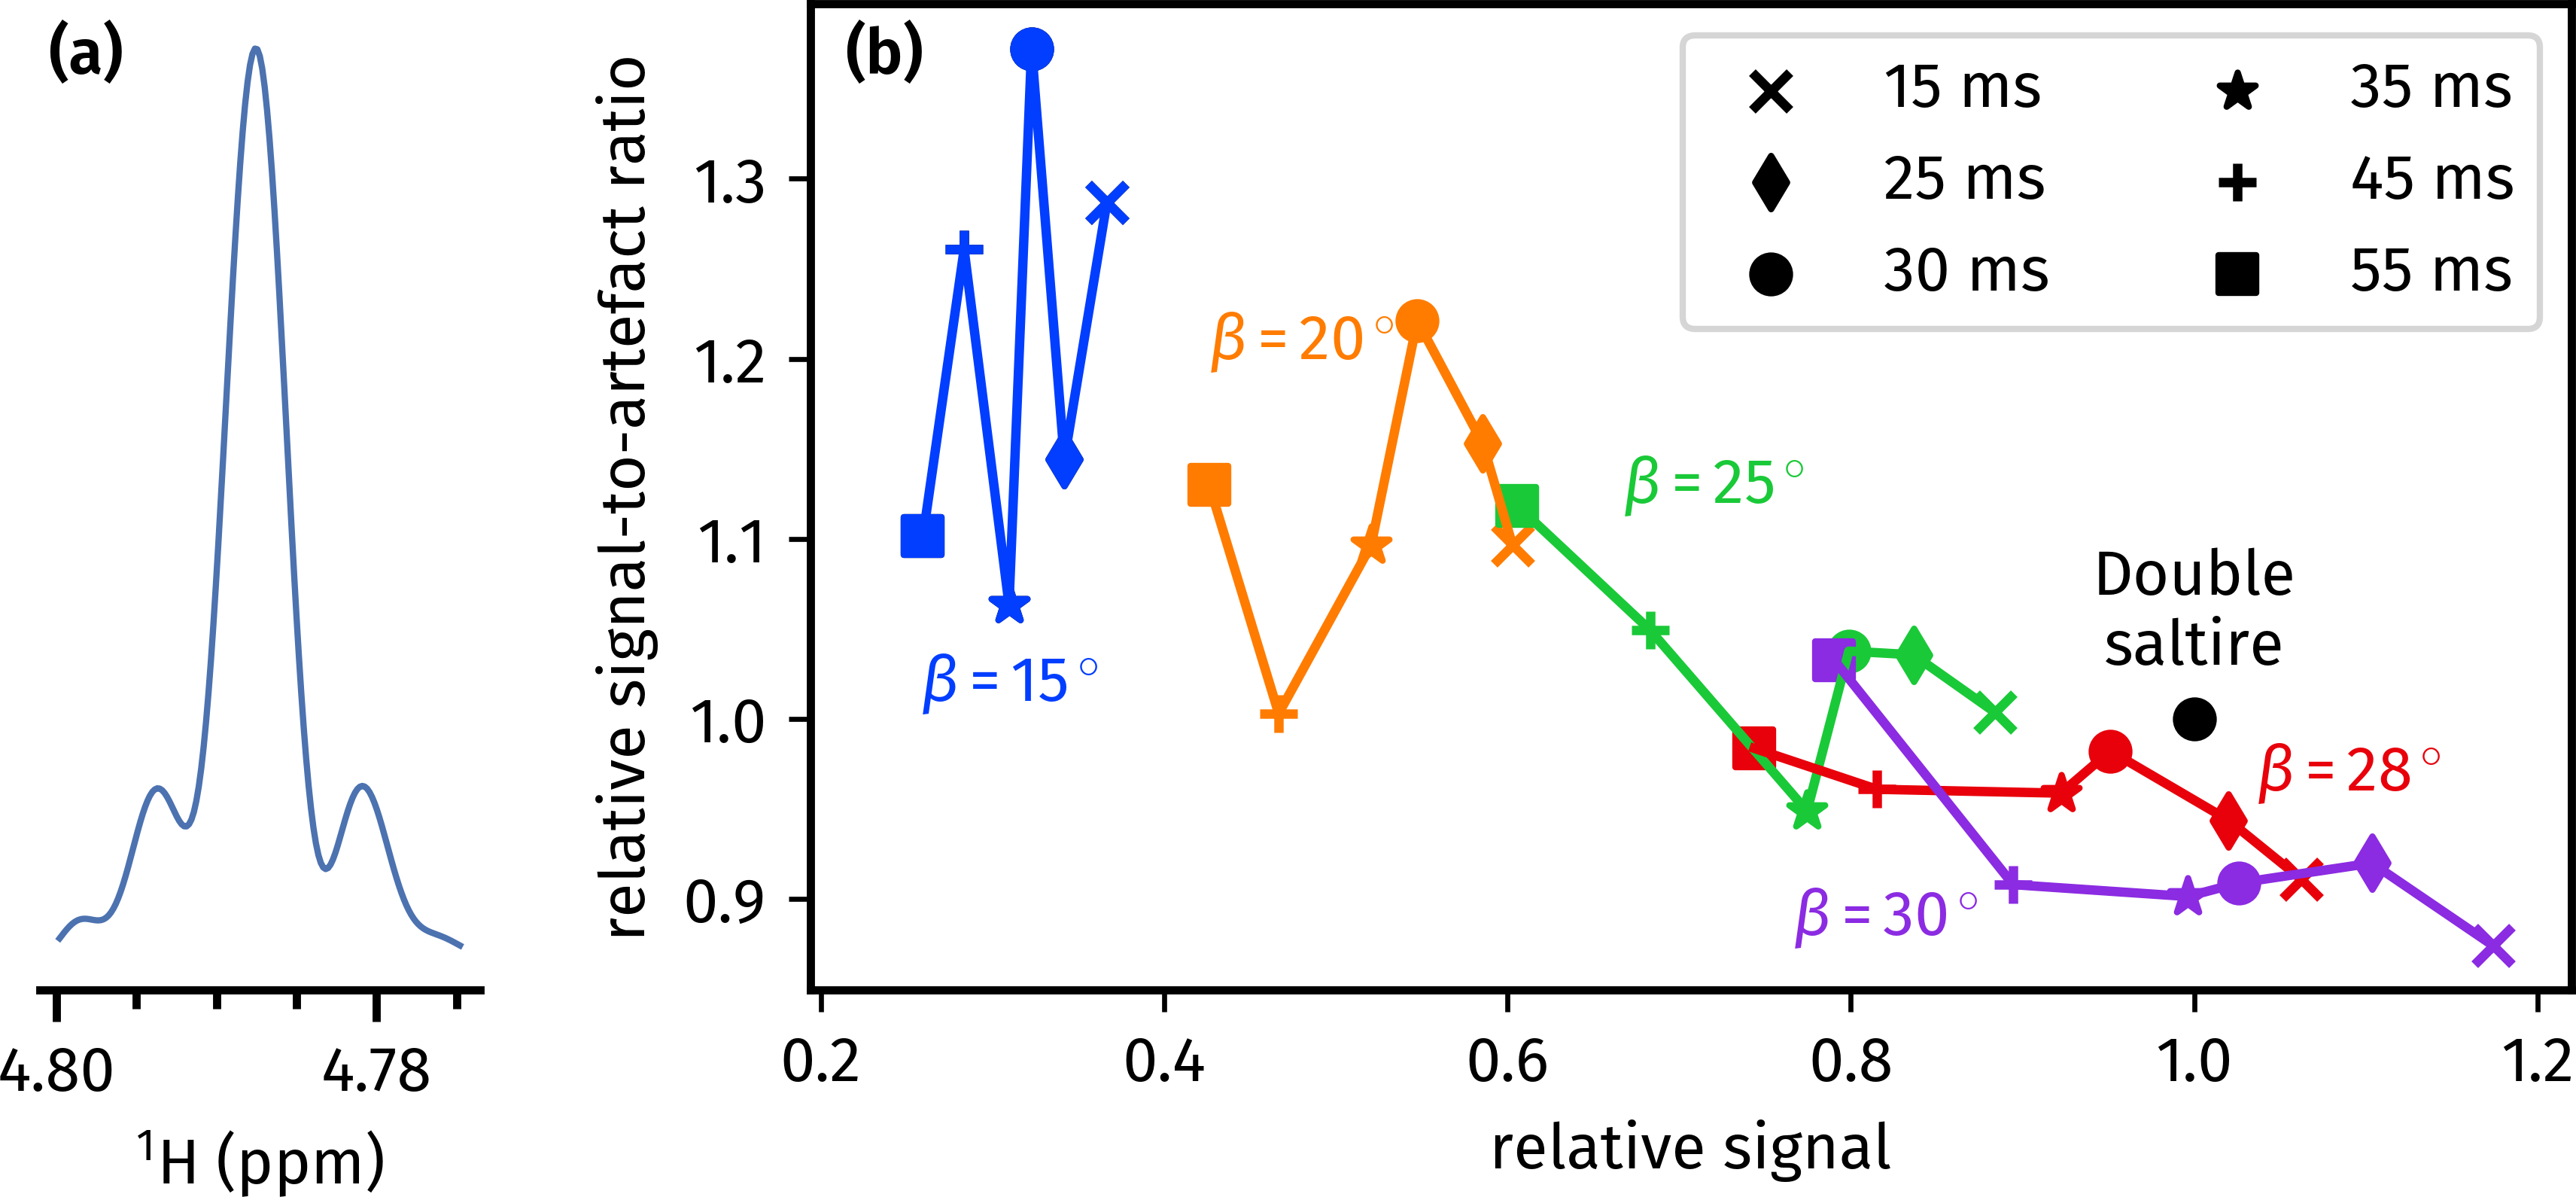
\includegraphics[]{pureshift/single_saltire.png}%
    {\phantomsubcaption\label{fig:single_saltire_results_spec}}%
    {\phantomsubcaption\label{fig:single_saltire_results_plot}}%
    \caption[Single-saltire PSYCHE results]{
        \textbf{(\subref{fig:single_saltire_results_spec})} The peak in the (reference, double-saltire) pure shift spectrum of cyclosporin used for calculation of signal intensity and signal-to-artefact ratio.
        \textbf{(\subref{fig:single_saltire_results_plot})} Plot showing the signal intensity and signal-to-artefact ratio obtained in various single-saltire PSYCHE experiments, normalised against the double saltire experiment with $\beta = \ang{20}$ and $\taup = \SI{30}{\ms}$.
        Each line represents a series of single-saltire experiments acquired with the same value of $\beta$; $\taup$ generally decreases going left to right (i.e.\ a longer pulse means less signal). 
        \datacode{5C-190617}
    }
    \label{fig:single_saltire_results}
\end{figure}

The results thus obtained are shown in \cref{fig:single_saltire_results_plot}.
In this plot, both the sensitivities as well as the signal-to-artefact ratios are normalised with respect to the reference double-saltire experiment (black dot at $(1, 1)$, acquired using $\beta = \ang{20}$ and a total $\taup = \SI{30}{\ms}$, i.e.\ \SI{15}{\ms} per saltire).
An ideal PSE would fall in the top-right corner of this plot.
Clearly, as the flip angle increases, the sensitivity increases but at the cost of the purity: this is hardly unsurprising given that the double-saltire experiment has the same property.
The effect of the pulse duration is less clear-cut: in general, a shorter PSE yields to increased signal, and very usable results were obtained even with a simple \SI{15}{\ms} single-saltire PSE.
However, a shorter PSE also leads to poorer spatiotemporal suppression of artefacts depends and thus poorer purity.

While there is no standout candidate which is \textit{clearly} better than the double saltire (i.e.\ greater sensitivity as well as purity), the single-saltire pulse with $\beta = \ang{28}$ and $\taup = \SI{30}{\ms}$ comes close in performance to the double-saltire experiment.
(The use of $\beta = \ang{28}$ here is not coincidental: this flip angle for a single saltire was chosen to (approximately) match the sensitivity of the $\beta = \ang{20}$ double-saltire experiment.)
Therefore, this does at least prove that a single saltire can be used as a PSE.
However, both the single- and quadruple-saltire cases suffer from the classic dilemma of pure shift NMR: just as in the original PSYCHE, and in the Zangger--Sterk method before it, there is a compromise between sensitivity and purity, and one can only be increased at the cost of the other.
Arguably, then, there is not much value in changing the number of saltire pulses as simply varying the \textit{flip angle} of the basic double-saltire already gives the experimentalist a way to balance these competing objectives.

\section{Direct optimisation of PSYCHE}
\label{sec:pureshift__optimisation}

This was stuff briefly pursued during my 2nd CDT rotation.
It didn't work very well---it's just insensible to try to optimise every point in a shaped pulse, and especially not experimentally.
But it did ultimately get expanded into POISE\ldots

\section{Time-reversal method}
\label{sec:pureshift__timerev}

This section focuses on the time-reversal element briefly introduced in \cref{subsec:pureshift__elements}: the aim is to determine whether a pure shift method based on this can have better performance than PSYCHE.
Before that, I will first provide a more detailed theoretical analysis of it.
The time-reversal element consists of just a single hard pulse with a flip angle $\beta$, and we first analyse its potential use as a JRE (instead of a PSE), using \cref{eq:ipm_beta_evolution,eq:ialpha_beta_evolution,eq:ibeta_beta_evolution}.

Recall that an ideal JRE should invert passive spins only, not active spins: thus, we seek a transformation of the form $I_{1+}I_{2\alpha} \to I_{1+}I_{2\beta}$.
However, the hard pulse does this:
\begin{equation}
    \label{eq:beta_pulse_not_jre}
    I_{1+}I_{2\alpha} \to
    {\underbrace{c^2s^2 I_{1+}I_{2\beta}}_{\text{term 1}}}
    + {\underbrace{c^4 I_{1+}I_{2\alpha}}_{\text{term 2}}}
    - {\underbrace{\frac{S^2}{4}I_{1\alpha}I_{2+} + \frac{S^2}{4}I_{1\beta}I_{2+}}_{\text{terms 3 and 4}}},
\end{equation}
where (as before) $S = \sin\beta$, $s = \sin(\beta/2)$, and $c = \cos(\beta/2)$.
As in the analysis for PSYCHE (\cref{subsec:pureshift__psyche_analysis}), term 1 here represents the desired signal; term 2 recoupling artefacts; and terms 3 and 4 COSY-type artefacts arising from coherence transfer.
Terms with difference coherence orders have been neglected as they can be removed using CTP gradients.\footnote{In the original work\autocite{Sorensen1985JACS} which predated widespread use of field gradients, other terms were removed through phase cycling, which is essentially equivalent.}
Unlike in the PSYCHE analysis, however, we have not neglected any other terms of smaller order in $s$.

Since the desired and undesired terms have different coefficients, it is possible to \textit{fully cancel out the recoupling artefacts} by recording (in this case) two different spectra with different values of $\beta$ and performing an appropriate linear combination:
\begin{align}
    I_{1+}I_{2\alpha} &\xrightarrow{\beta = \ang{0}} I_{1+}I_{2\alpha} \label{eq:timereversal_twospin_0} \\
    I_{1+}I_{2\alpha} &\xrightarrow{\beta = \ang{90}} \frac{1}{4}I_{1+}I_{2\beta} + \frac{1}{4}I_{1+}I_{2\alpha} - \frac{1}{4}I_{1\alpha}I_{2+} + \frac{1}{4}I_{1\beta}I_{2+} \label{eq:timereversal_twospin_90}
\end{align}
If we take \cref{eq:timereversal_twospin_90} minus $1/4$ of \cref{eq:timereversal_twospin_0}, the recoupling artefacts (arising from the $I_{1+}I_{2\alpha}$ term) are fully removed.
In general, for an $N$-spin system, there are several different `types' of recoupling artefacts where different numbers of passive spins (between 1 and $N - 1$) are not inverted.
Each of these pathways will have different coefficients, as each spin that is flipped contributes $s^2$, whereas each spin that is not flipped contributes $c^2$.
Suppressing all of these requires the acquisition and summation of $N$ spectra with different flip angles and appropriate weights.

Before we go on further, notice even in the two-spin system that the COSY-type artefacts are \textit{not} suppressed!
In the original work\autocite{Sorensen1985JACS}, this time-reversal element was used in the middle of the $t_1$ period in a NOESY experiment.
The coherence transfer peaks were not deemed to be problematic in this context: they gave rise to artefacts which had $F_1$ frequencies of $(\Omega_1 + \Omega_2)/2$, but different phase properties to genuine crosspeaks, allowing them to be easily identified.
Of course, these artefacts are not acceptable in an actual pure shift spectrum.

To remove these peaks, I adopted the strategy first reported by Thrippleton \textit{et al.} for suppression of COSY-type transfer pathways in 2DJ spectra.\autocite{Thrippleton2005JMR}
In a 2DJ experiment, the central \ang{180} pulse should in principle not cause coherence transfers between different spins; however, in strongly coupled systems this can happen.
The solution was to bracket the \ang{180} pulse, as well as half of the $t_1$ period, with a pair of opposing chirps and gradients.
The same idea was later used in the TSE-PSYCHE experiment\autocite{Foroozandeh2015CC} to (further) suppress strong coupling responses in the parent PSYCHE experiment.
This works because the unwanted CTPs have coherences on different spins during each of the two chirps; consequently, the coherences are inverted at different times by the chirp pulses, and are ultimately dephased by gradients.
The resulting time-reversal experiment was thus simply the same as the parent TSE-PSYCHE experiment, except that the central PSYCHE element was replaced by a $\beta$ hard pulse (\cref{fig:timereversal_pulseq}).

\begin{figure}[htb]
    \centering
    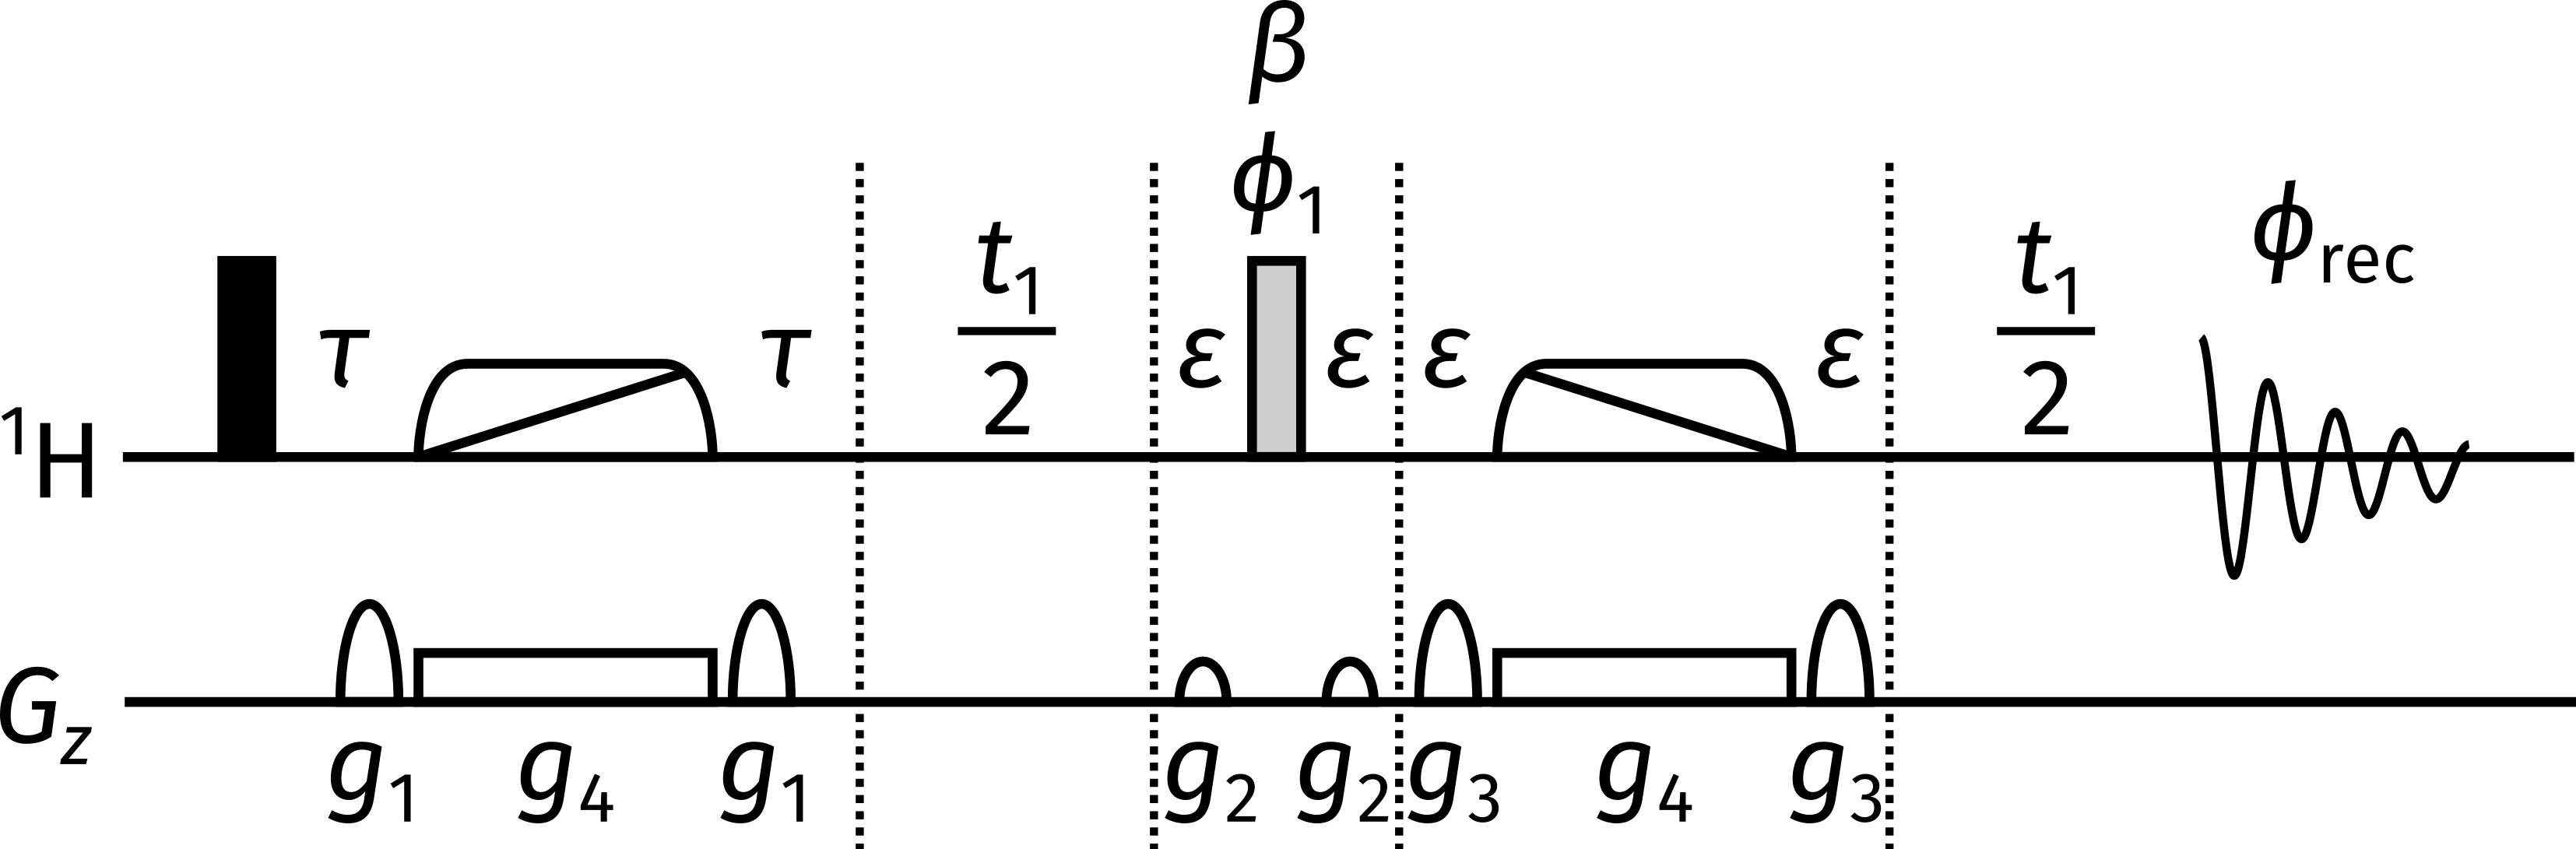
\includegraphics[]{pp/pureshift/timereversal.png}%
    \caption[Time-reversal pure shift pulse sequence]{
        Time-reversal pure shift pulse sequence.
        The flip angle $\beta$ is varied as described in \cref{eq:timereversal_pse_angles}.
        Pulse phases are: $\phi_1 = (x, y, -x, -y)$; $\phi_\text{rec} = (x, -x, x, -x)$.
        The delay $\tau$ is set to $1/(4 \cdot T_\text{chunk})$, and allows for J-coupling to be refocused in the middle of the chunk.
        Gradient amplitudes are $(g_1, g_2, g_3, g_4) = (35\%, 49\%, 77\%, 1\%)$ (note that, in principle, $g_4$ should be calibrated according to the bandwidth of the chirp used).
    }
    \label{fig:timereversal_pulseq}
\end{figure}

In such a sequence, the JRE is in fact not only the $\beta$ pulse itself but also the second chirp (which effectively acts as a \ang{180} pulse).
So, the $\beta$ pulse here fulfils the role of a PSE, not a JRE: this means that different flip angles and weights must be chosen.
As before, for a system containing $N$ mutually coupled spins, $N$ different experiments must be acquired using the following flip angles $\beta_j$ and summed with the corresponding weights $W_j$ ($j = 1, 2, \ldots, N$):
\begin{align}
    \beta_j &= \frac{j\pi}{N} \label{eq:timereversal_pse_angles} \\
    W_j &= \frac{N}{8}\cdot \frac{(-1)^j}{\sin^2(\beta_j/2)} \label{eq:timereversal_pse_weights}.
\end{align}
For the sake of completeness, the values of $\beta$ and $W$ for a JRE are given here as well:
\begin{align}
    \beta_k &= \frac{k\pi}{N} \label{eq:timereversal_jre_angles} \\
    W_k &= \frac{N}{8}\cdot \frac{(-1)^{k + N}}{\cos^2(\beta_j/2)} \label{eq:timereversal_jre_weights}
\end{align}
for $k = 0, 1, \ldots, N-1$.
The derivation of these expressions is discussed more thoroughly in a paper by Griesinger et al.\autocite{Griesinger1986JCP}
In the context of this specific paper, note that the weights for the PSE correspond to that used for the ECOSY experiment, and the weights for the JRE correspond to that used for the complementary ECOSY experiment.

In practice, $N = 5$ is likely to cover most realistic spin systems.
Explicitly evaluating \cref{eq:timereversal_pse_angles,eq:timereversal_pse_weights} yields $\beta = \{\ang{36}, \ang{72}, \ang{108}, \ang{144}, \ang{180}\}$ and $W = \{−6.545,1.809,−0.955,0.691,−0.625\}$.
\Cref{fig:timereversal_insets} shows insets of the five subspectra acquired with the above values of $\beta$ and scaled by their respective weights $W$.
The weighted sum (i.e.\ the pure shift spectrum) was phased, and the resulting phase correction values were propagated back to the individual subspectra.

\begin{figure}[htb]
    \centering
    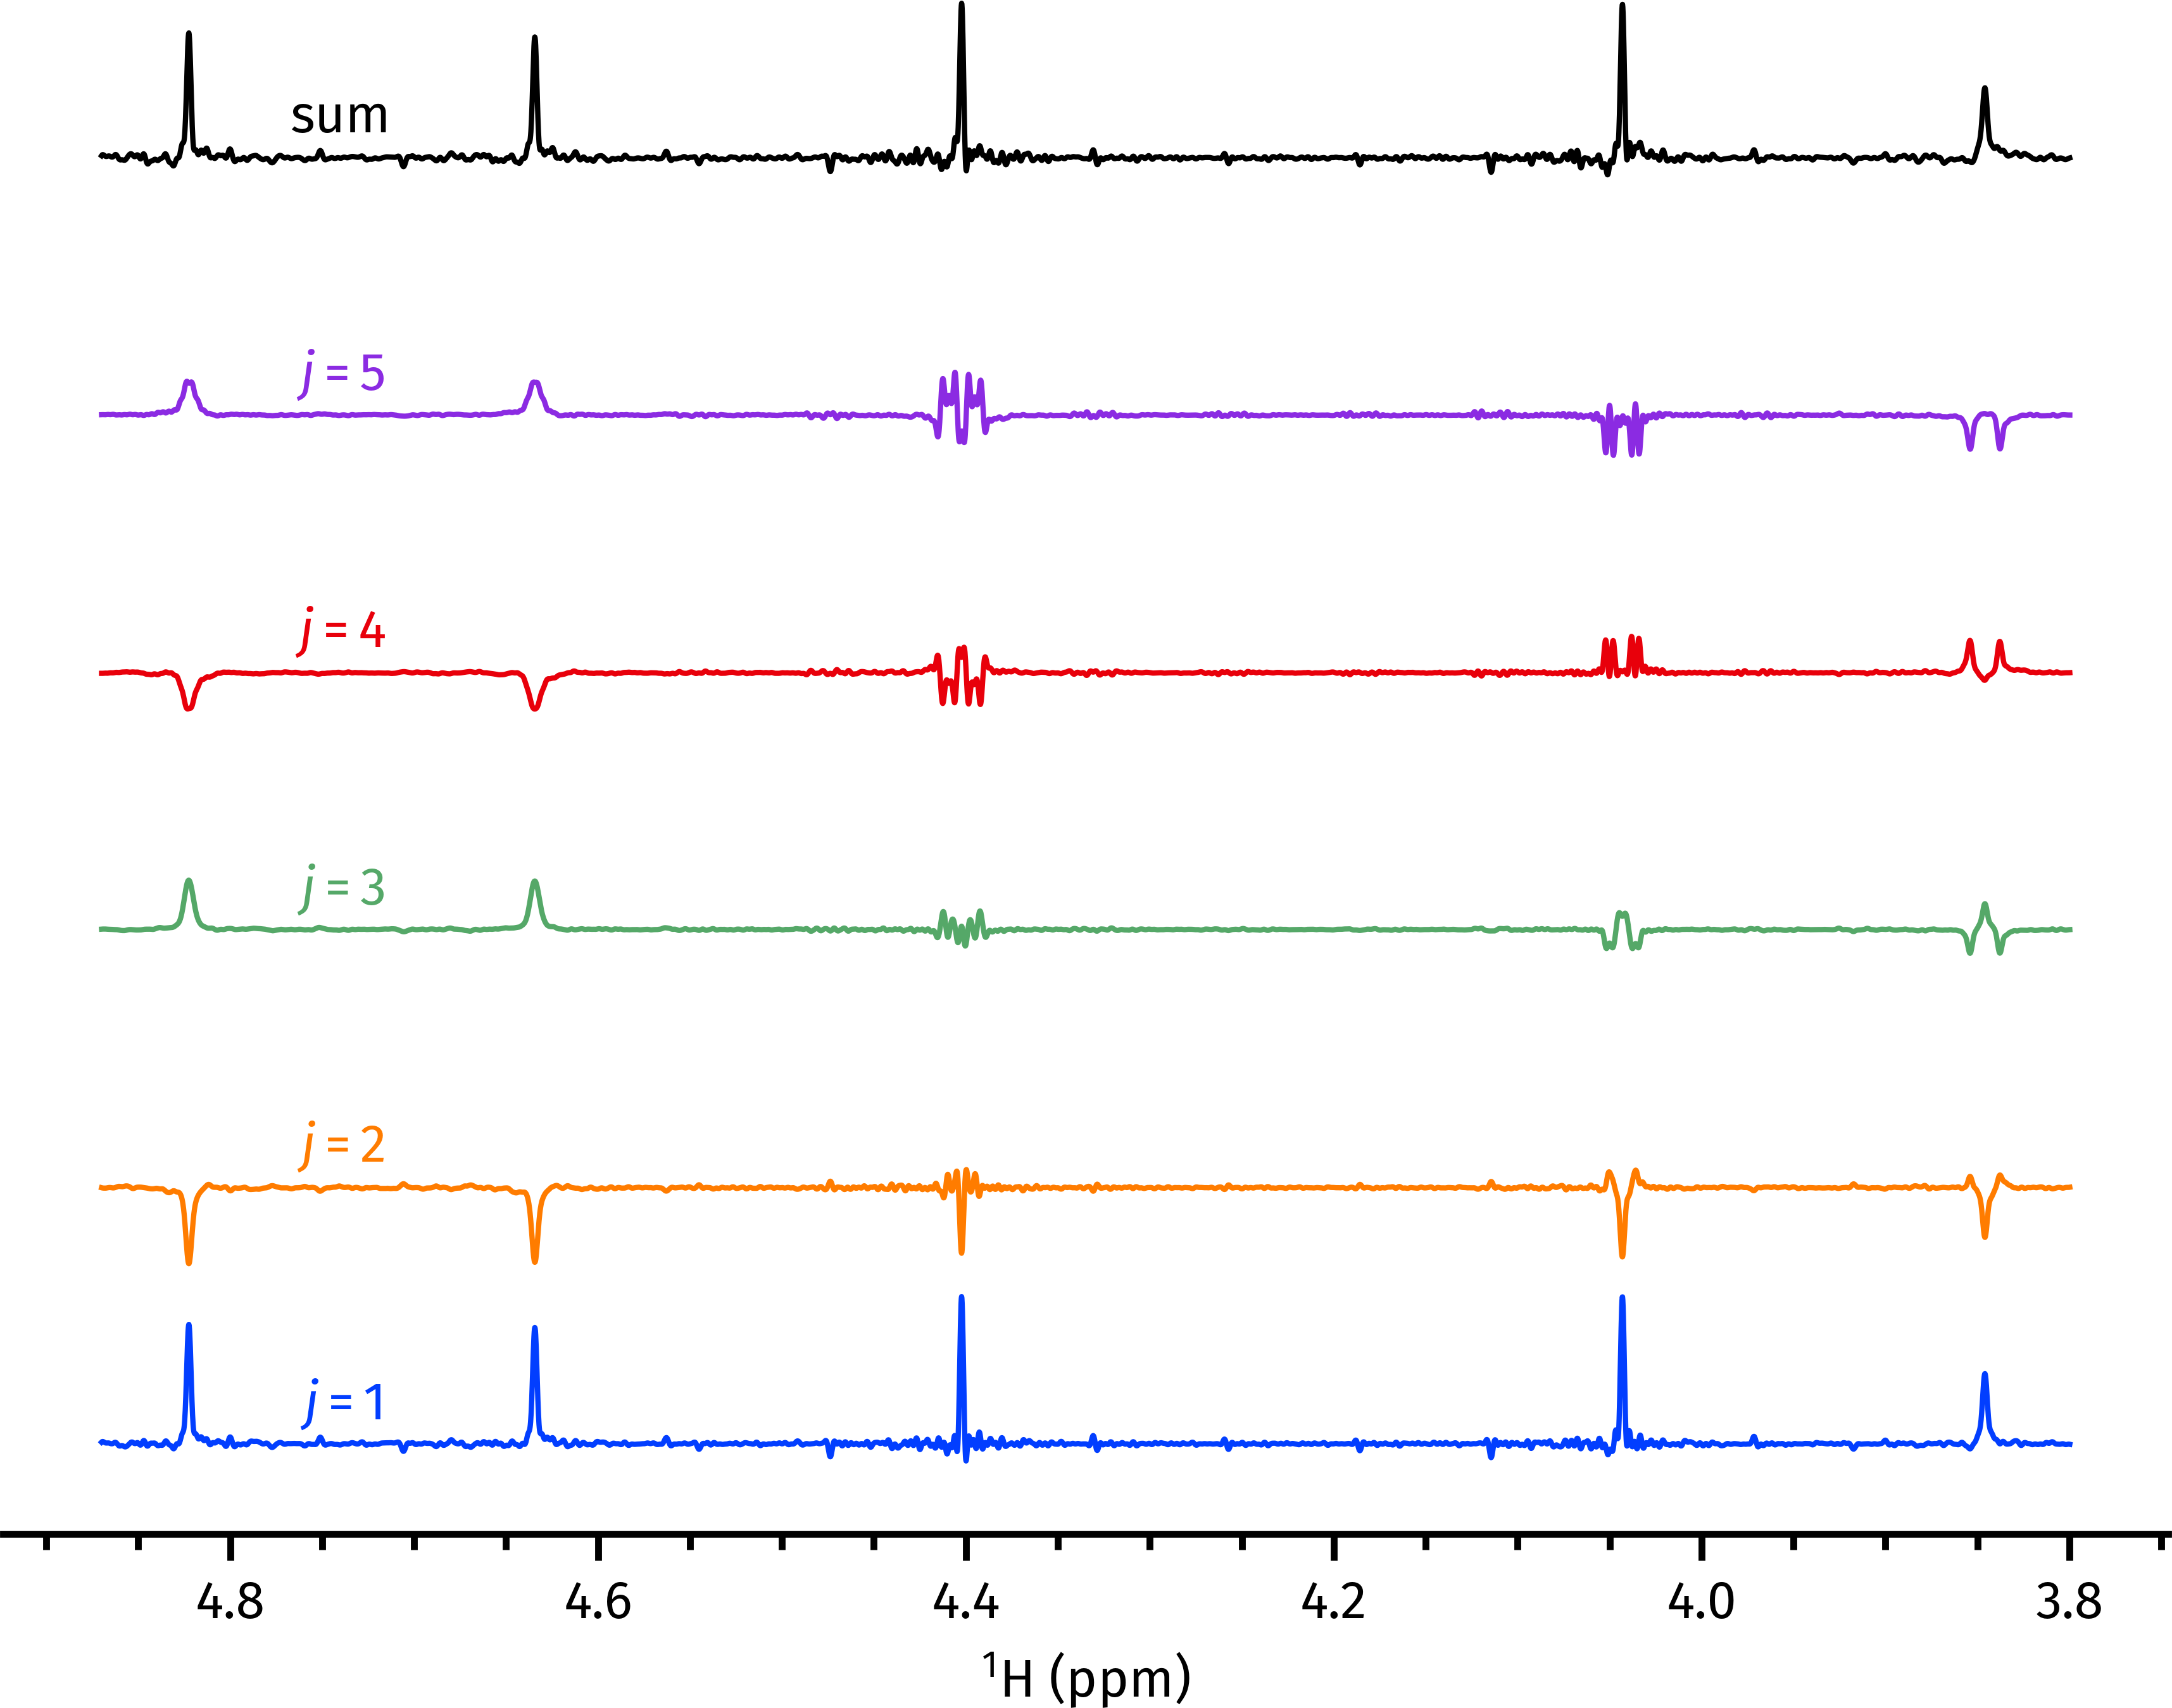
\includegraphics[]{pureshift/timereversal_insets.png}%
    \caption[Insets of time-reversal spectra]{
        Insets of weighted time-reversal subspectra (with $j = 1$ through 5), as well as their sum (the pure shift spectrum).
        \datacode{7A-201020}
    }
    \label{fig:timereversal_insets}
\end{figure}

Although the experiment seems to work, in that the weighted sum \textit{is} indeed a pure shift spectrum, the fact that it is obtained through summation of $N$ different experiments brings some immediate drawbacks.
Firstly, the minimum duration of the experiment is lengthened by a factor of $N$: this is essentially the same as an $N$-step phase cycle.
However, and perhaps more importantly in the context of \textit{pure shift} NMR, the artefacts surrounding the main peaks are not perfectly cancelled through the process of summation.
As a result, random distortions are observed around the desired peaks in the pure shift spectrum: this is noticeable in the \SI{4.04}{ppm} peak in \cref{fig:timereversal_insets}, and is even worse for more intense signals.

In terms of sensitivity, the time-reversal spectrum is not particularly exceptional, either.
Each of the five subspectra above were acquired with 2 scans; when compared against a typical TSE-PSYCHE experiment acquired with only 4 scans (i.e.\ 40\% of the experiment duration), the TSE-PSYCHE experiment had comparable or perhaps even slightly better SNR (\cref{fig:timereversal_sensitivity}).
The likely reason for this is because in the time-reversal experiment, signal is actually being \textit{cancelled out} through the process of summation, as is quite clearly shown in \cref{fig:timereversal_insets}.
In principle, the sensitivity of the time-reversal experiment could be optimised by acquiring the more heavily weighted spectra with more scans.
However, I consider this unlikely to make a substantial difference to the conclusions drawn here.
The idea of re-optimising the weights to better suppress artefacts was also briefly considered.
However, given that \cref{eq:timereversal_pse_weights} already yields \textit{theoretically} complete suppression, it was deemed unlikely that anything substantially better could be obtained, considering that the artefacts arise from the summation process itself and are likely to appear regardless of what weights are chosen.
Performing such an optimisation would also require a pure shift spectrum to have been acquired beforehand (for comparison), thus defeating the purpose of optimising the weights anyway.

\begin{figure}[htb]
    \centering
    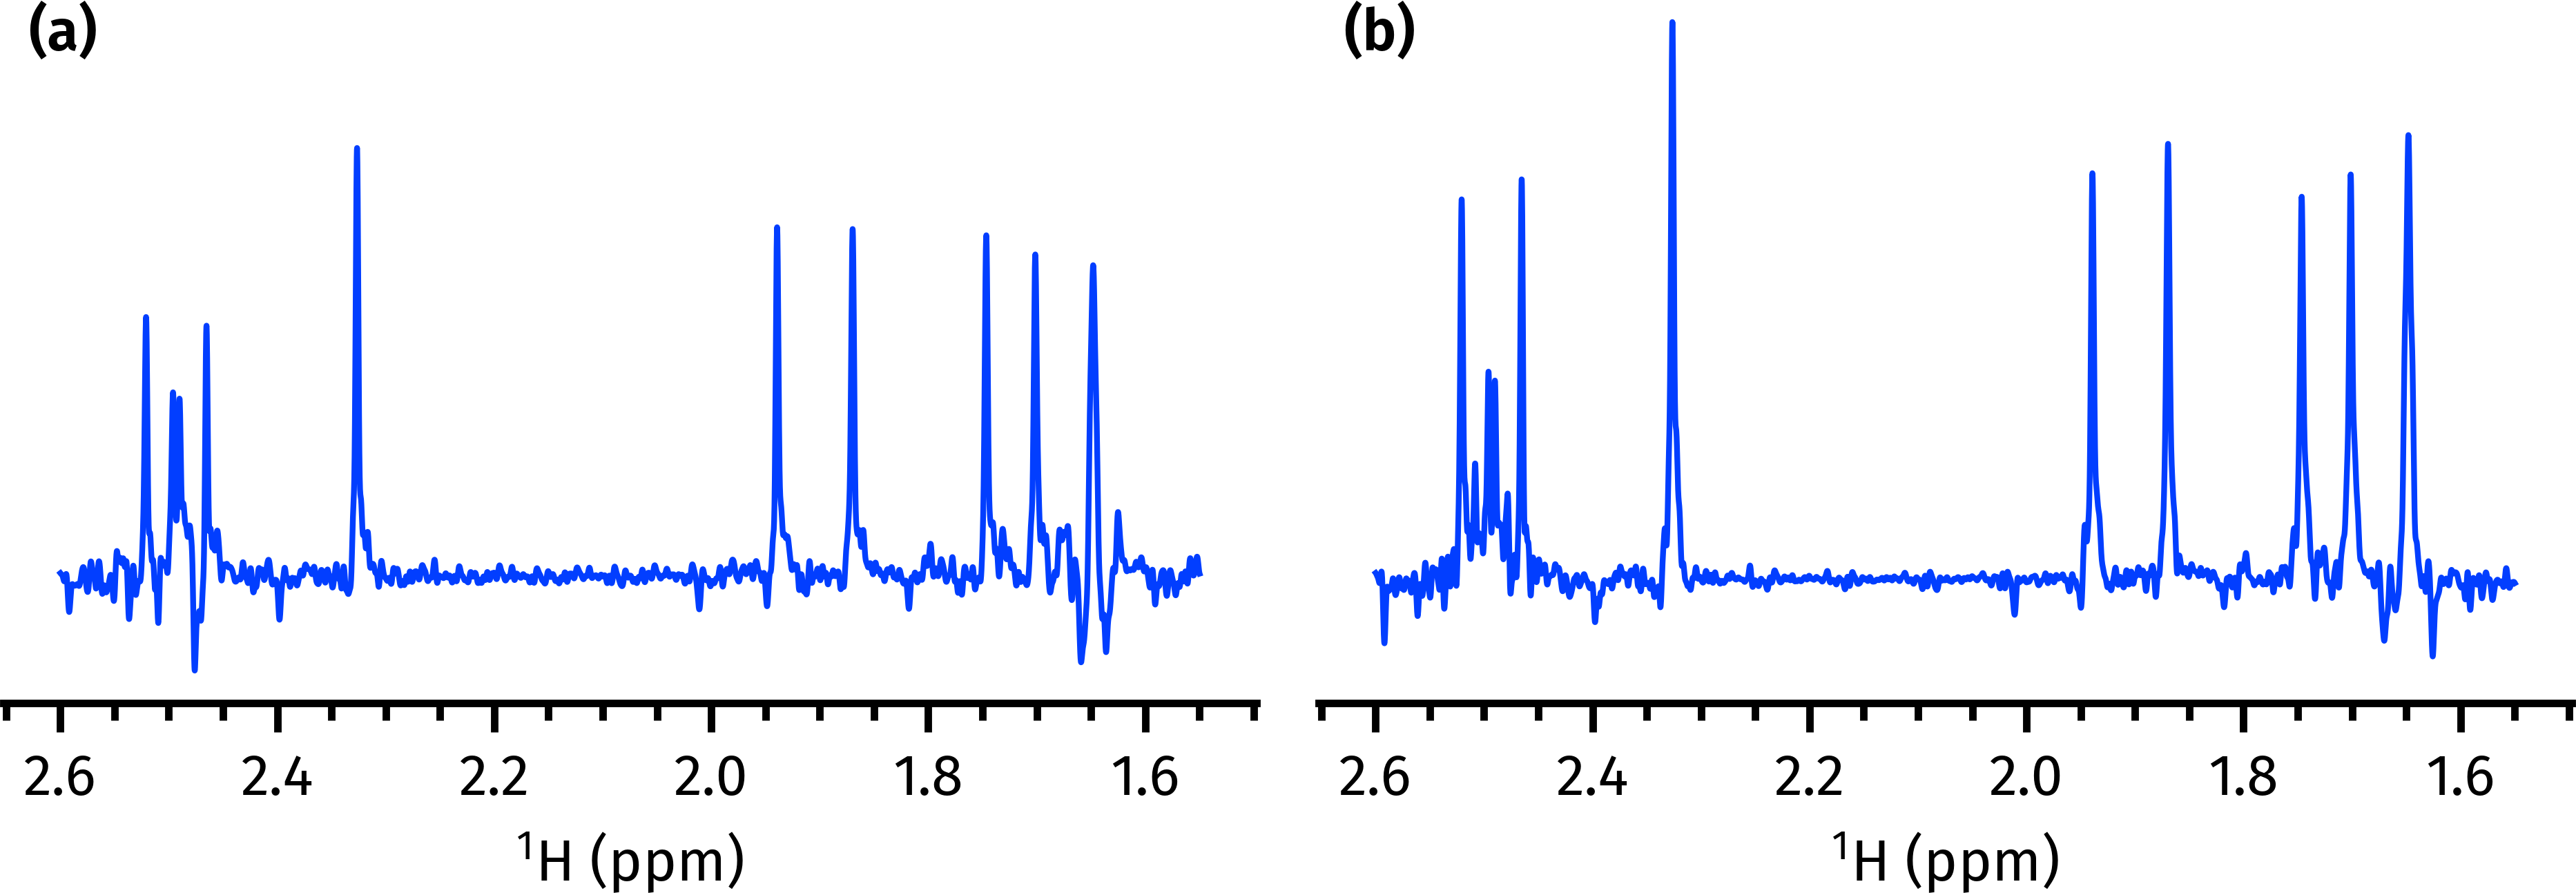
\includegraphics[]{pureshift/timereversal_sensitivity.png}%
    {\phantomsubcaption\label{fig:timereversal_sensitivity_tr}}%
    {\phantomsubcaption\label{fig:timereversal_sensitivity_tsepsyche}}%
    \caption[Comparison of time-reversal and TSE-PSYCHE sensitivity]{
        Comparison of time-reversal and TSE-PSYCHE sensitivity.
        \textbf{(\subref{fig:timereversal_sensitivity_tr})} Time-reversal pure shift spectrum (the same as the sum in \cref{fig:timereversal_insets}) acquired with 2 scans for each subspectrum.
        \textbf{(\subref{fig:timereversal_sensitivity_tsepsyche})} TSE-PSYCHE (double saltire, flip angle \ang{15}) acquired with 4 scans.
        The spectra have been scaled so that their noise levels are similar: the signal intensity is comparable, or perhaps slightly better in the TSE-PSYCHE.
        \datacode{7A-201020}
    }
    \label{fig:timereversal_sensitivity}
\end{figure}

Interestingly, \cref{fig:timereversal_insets} suggests that the $j = 1$ spectrum \textit{on its own} already provides as good a result as the summed pure shift spectrum.
This is not surprising, as the use of a hard pulse as the PSE yields a conceptually very similar result to PSYCHE in that the signal to artefact ratio depends on $\tan^2(\beta/2)$ (of course, the COSY-type artefacts must still be suppressed through the TSE scheme).
This suggests that even without summation of multiple subspectra, the TSE time-reversal pulse sequence in \cref{fig:timereversal_pulseq} is a viable pure shift experiment---albeit one which does not have any significant advantage over PSYCHE.

\section{`Discrete PSYCHE'}
\label{sec:pureshift__dpsyche}

The last pure shift method in this chapter is completely original, and represents perhaps the most fruitful attempt so far at optimising pure shift experiments.
It relies on what is essentially a `temporal discretisation' of the PSYCHE waveform and gradient combination: instead of applying a shaped pulse and a gradient simultaneously, hard pulses and gradients are interleaved in the PSE (\cref{fig:dpsyche_pulseq}).

\begin{figure}[htb]
    \centering
    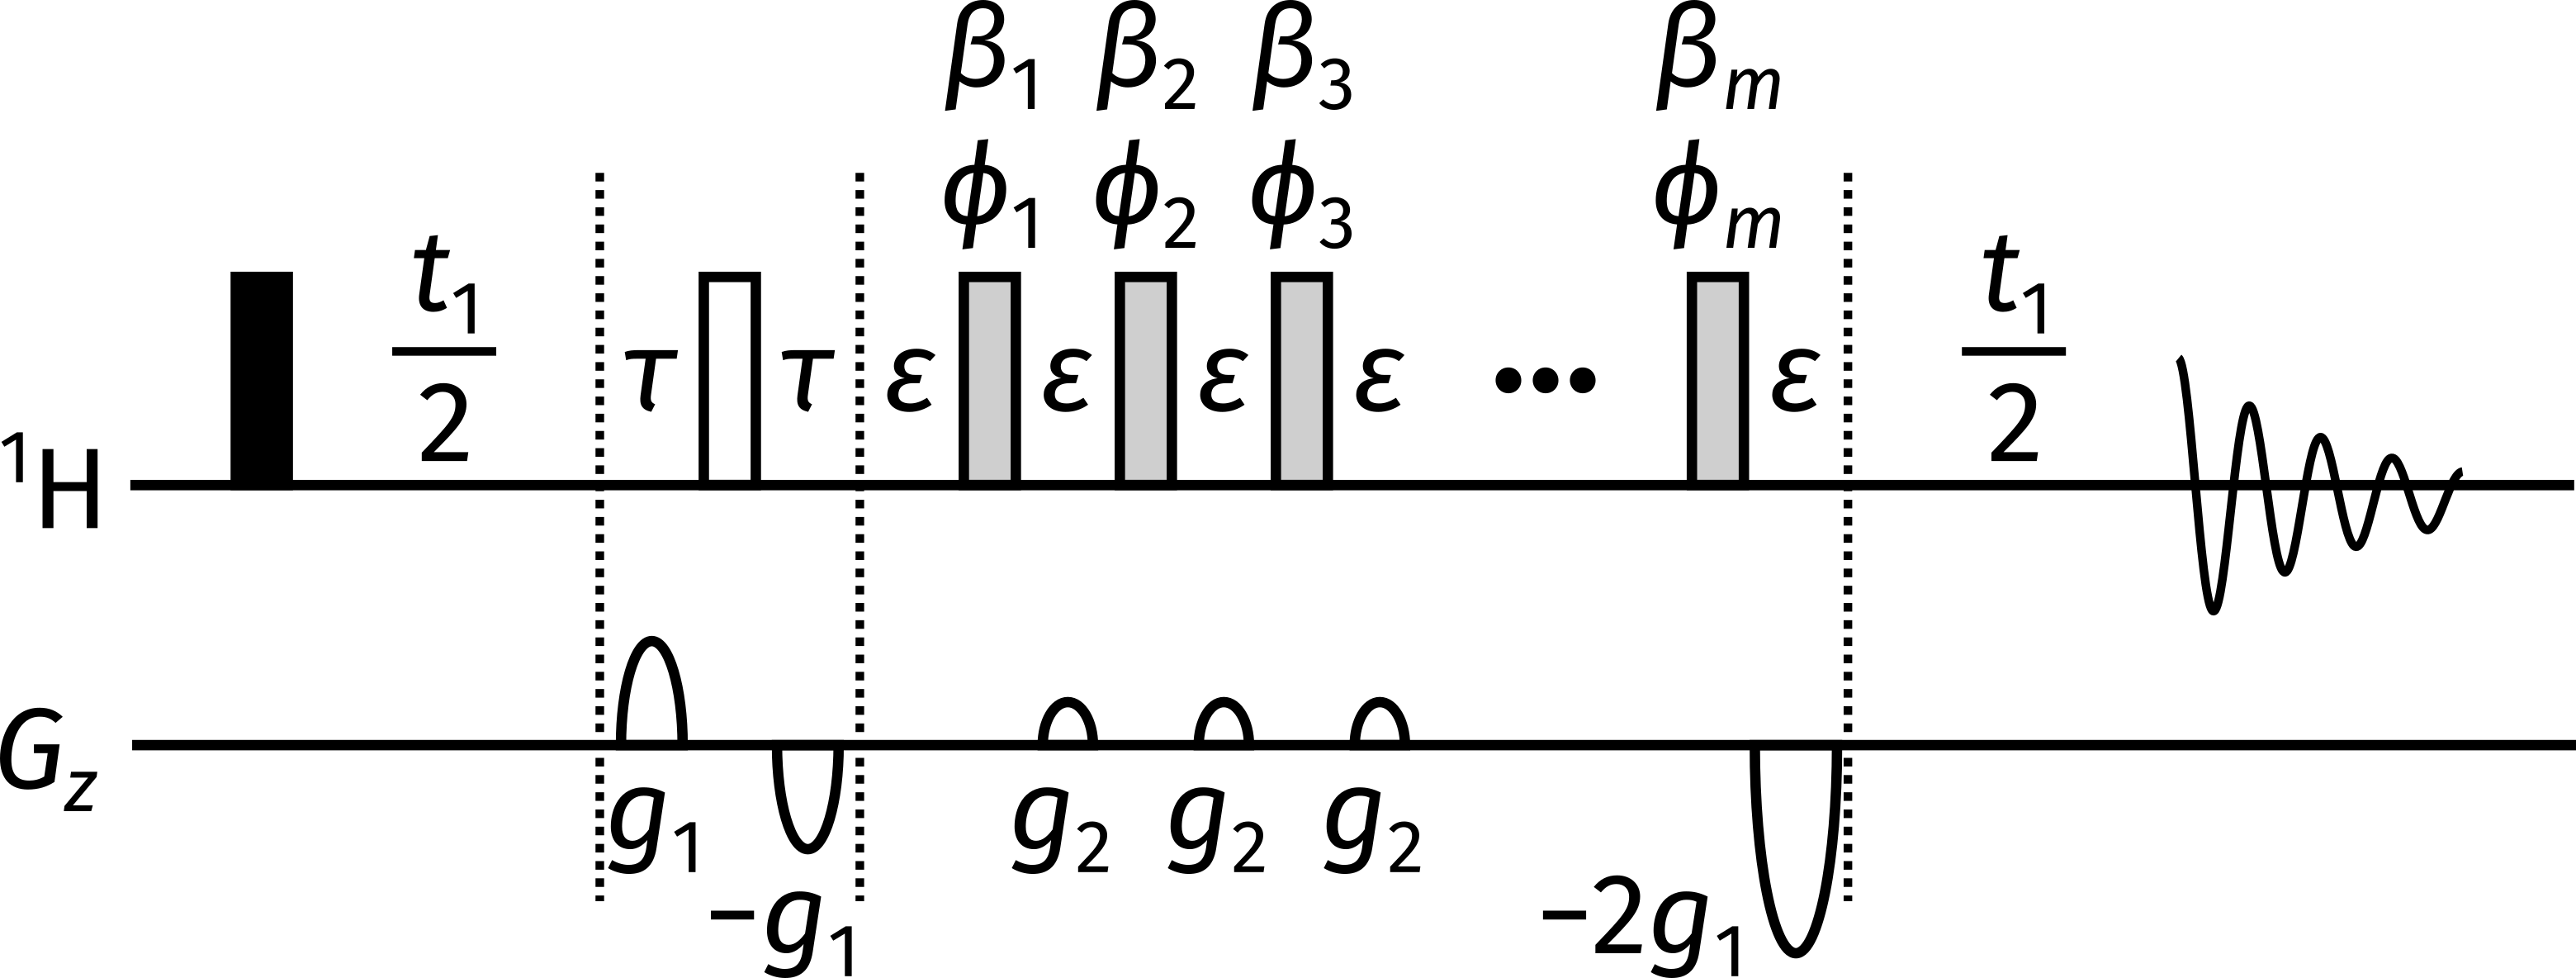
\includegraphics[]{pp/pureshift/dpsyche.png}%
    \caption[dPSYCHE pulse sequence]{
        dPSYCHE pulse sequence.
        Gradient amplitudes are $(g_1, g_2) = (35\%, 41\%)$; the gradients in the PSE $g_2$ are applied with a duration of \qty{500}{\us}.
        The hard pulses in the PSE are applied with an RF amplitude of \qty{18}{\kHz}.
        The delay $\tau$ is set to $1/(4 \cdot \Tchunk)$, and allows for J-coupling to be refocused in the middle of the chunk.
    }
    \label{fig:dpsyche_pulseq}
\end{figure}

For this reason I have dubbed this experiment the `discrete PSYCHE', or dPSYCHE for short.
There are two major reasons why this is more amenable towards optimisation than many of the previous experiments:
\begin{enumerate}
    \item Pulses and gradients are no longer applied simultaneously, which makes simulation of the experiment \textit{extremely} fast compared to the original PSYCHE.
        This opens up the possibility of entirely theoretical optimisations, as the noise can be completely eliminated from the cost function.
        
    \item There are much fewer `pulse points' than in the original PSYCHE: effectively, the phase and flip angle of every hard pulse has to be optimised, leading to $2m$ parameters.
        Even for $m \sim 10$, this is quite tractable if the optimisation is noiseless.
\end{enumerate}

One downside of this is that it is difficult, or perhaps even impossible, to explain how the PSE works.%
\footnote{Of course, we could simulate it and say that it works because the maths says it does; but that isn't very illuminating. Some of the optimisations done in this thesis are somewhat like a scaled-down version of machine learning, in that they produce better results at the cost of interpretability.}
For a symmetric PSE where $\beta_1 = \beta_m$ (and so on) it is probably possible to reuse an explanation based on PSYCHE-style CTP selection, but this is clearly inapplicable if the flip angles and phases are scrambled.

\subsection{Speeding up dPSYCHE simulations}
\label{subsec:pureshift__dpsyche_simulations}

To begin, I first explain how the exact simulation of dPSYCHE experiments can be greatly accelerated through efficient propagator calculations.
Although Spinach\autocite{Hogben2011JMR} is the leading simulation package for NMR, and covers an extremely impressive range of experiments, this generality also prevents it from providing optimal performance for any single experiment.
As it turns out, handwritten, specialised Matlab code can outperform Spinach by orders of magnitude.

The NMR simulations developed here simply use the density operator formalism in Hilbert space, as outlined in \cref{sec:theory__density_operators}.
The Zeeman basis is used, and non-unitary transformations such as relaxation are neglected.
Propagation under the Liouville--von Neumann equation (\cref{eq:lvn_interaction_integrated}) requires the calculation of matrix exponentials $\exp(-\mi H\tau)$.
For an $N \times N$ matrix, the matrix exponential requires $O(N^3)$ time to calculate (and for a system containing $p$ spins, we have $N = 2^p$); it is often this which is the bottleneck in NMR simulations.
Minimising the number of matrix exponentials, and/or their computational cost, is the key to achieving speedups, as will be shown in the following text.%
\footnote{Note that in my simulations, I simply used the builtin \texttt{expm} Matlab function, which implements the matrix exponential using a combination of the scaling-and-squaring method and Pad\'e approximation\autocite{Higham2005SIAMJMAA}.
This is in contrast to Spinach, which primarily uses a scaled-and-squared Taylor series (according to the \texttt{propagator.m} file, various other methods supposedly did not `live up to their marketing').
An in-depth discussion of matrix exponential methods is outside the scope of this thesis, but can be found in a classic paper by Moler and Van Loan\autocite{Moler2003SIAMR}.}

Generally, the accurate simulation of pulsed field gradients requires the sample to be divided up into $n$ discrete slices, each simulated with a different $\Hgrad$.\footnote{In simple cases this can be avoided by simply removing all terms with the wrong coherence orders as we know they will be dephased (\cref{eq:generalised_rephasing_2}), but this is too naive an approach for pure shift techniques.}
Thus, a very naive implementation of the dPSYCHE experiment would require $mn$ matrix exponentials, one per pulse per slice.
The overall structure of the code would resemble \cref{lst:dpsyche_slow}.%
\footnote{Strictly speaking, there is a slight inaccuracy in this code: the final gradient should have strength \texttt{-2G} and not \texttt{G}, but that is a minor detail which I leave out for clarity in the code.}
Note that the term \texttt{H\_free}, and the corresponding propagator \texttt{U\_free}, technically refer to the interaction-picture free Hamiltonian, $\HfreeI$.

\begin{mylisting}[htb]
    \centering
\begin{tcbminted}{matlab}
% loop over slices
for slce=1:n
    H_grad = I_z * G * z(slce);

    % loop over pulse points
    for pulse_point=1:m
        H_pulse = (c_x(pulse_point) * I_x) + (c_y(pulse_point) * I_y);

        % calculate propagators; m*n total matrix exponentials
        U_pulse = expm(-1j * (H_free + H_pulse) * t_pulse);
        U_grad = expm(-1j * (H_free + H_grad) * t_grad);

        rho = U_grad * U_pulse * rho * U_pulse' * U_grad';
    end
end
\end{tcbminted}
\caption[Naive dPSYCHE code]{Rough structure of a naive dPSYCHE implementation. Note that I use the variable name \texttt{slce} as \texttt{slice} is an existing builtin Matlab function.}
\label{lst:dpsyche_slow}
\end{mylisting}

It is not difficult to come up with a more sensible approach which cuts this down by a factor of $m$: since the pulses are not applied together with the gradients, the pulse propagators $U_{\symup{pulse}}$ can be pre-calculated outside of the loop.
Furthermore, all of the gradients within the PSE are the same, so $U_{\symup{grad}}$ can be moved out of the inner loop (\cref{lst:dpsyche_fast1}).

\begin{mylisting}[htb]
    \centering
\begin{tcbminted}{matlab}
% precalculate pulse propagators; m total matrix exponentials
for pulse_point=1:m
    H_pulse = (c_x(pulse_point) * I_x) + (c_y(pulse_point) * I_y);
    U_pulse(m) = expm(-1j * (H_free + H_pulse) * t_pulse);
end

% loop over slices
for slce=1:n
    % calculate gradient propagators; n total matrix exponentials
    H_grad = I_z * G * z(slce);
    U_grad = expm(-1j * (H_free + H_grad) * t_grad);
    
    % loop over pulse points
    for point=1:m
        rho = U_pulse(m) * rho * U_pulse(m)';
        rho = U_grad * rho * U_grad';
    end
end
\end{tcbminted}
\caption[Slightly faster dPSYCHE code]{Rough structure of a slightly faster implementation of dPSYCHE.}
\label{lst:dpsyche_fast1}
\end{mylisting}

Spinach, which is designed to be general, has no idea that these optimisations are possible, so is naturally rather slower.
However, even this is relatively inefficient.
It can be shown that the two components of the gradient propagator, $\HfreeI$ and $\Hgrad$, actually commute with one another (even in the strong coupling case).
Thus, we can write:
\begin{equation}
    \label{eq:split_propagator}
    \exp[-\mi(\HfreeI + \Hgrad)\tau] = \exp(-\mi\HfreeI\tau) \exp(-\mi\Hgrad\tau)
\end{equation}
(in general, for matrices $A$ and $B$, $\exp(A + B) = \exp(A)\exp(B)$ if and only if $[A, B] = 0$).
This on its own does not reduce the number of matrix exponentials required, but notice now that $\Hgrad$ is a sum of $I_{iz}$ terms and is therefore \textit{diagonal} in the Zeeman basis.
The exponential of a diagonal matrix is almost trivial to calculate, as we only need to exponentiate the diagonal \textit{elements:}
\begin{equation}
    \label{eq:expm_diagonal}
    \exp
    \begin{pmatrix}
        \lambda_1 & 0 & \ldots & 0 \\
        0 & \lambda_2 & \ldots & 0 \\
        \vdots & \vdots & \ddots & \vdots \\
        0 & 0 & \ldots & \lambda_n \\
    \end{pmatrix}
    = 
    \begin{pmatrix}
        \exp(\lambda_1) & 0 & \ldots & 0 \\
        0 & \exp(\lambda_2) & \ldots & 0 \\
        \vdots & \vdots & \ddots & \vdots \\
        0 & 0 & \ldots & \exp(\lambda_n) \\
    \end{pmatrix}.
\end{equation}
Instead of using the $O(N^3)$ \texttt{expm(M)} function, this can instead be done in $O(N)$ time using \texttt{diag(exp(diag(M)))} (the \texttt{diag} Matlab function converts a diagonal matrix to a vector of its diagonal entries, and vice versa).
So, we now require only $m + 1$ `true' matrix exponentials.
At this point, our matrix exponentials have almost been eliminated and the largest remaining bottleneck is almost certainly the matrix \textit{multiplications} required for the propagation.
We can cut these down by a factor of two simply by calculating the overall propagator
\begin{equation}
    \label{eq:overall_propagator}
    U_{\symup{total}} = U_n\cdots U_2U_1
\end{equation}
and then performing the propagation only at the very end:
\begin{equation}
    \label{eq:overall_propagation}
    \rho = U_{\symup{total}} \rho_0 \adj{U_{\symup{total}}}
\end{equation}
instead of performing every individual step $\rho \to U_1\rho_0\adj{U_1}$.
The final optimised code therefore resembles that in \cref{lst:dpsyche_fast2}.

\begin{mylisting}[htb]
    \centering
\begin{tcbminted}{matlab}
% precalculate propagator due to free evolution during gradient
% only 1 matrix exponential
U_free = expm(-1i * H_free * t_grad);

% precalculate pulse propagators; m total matrix exponentials
for pulse_point=1:m
    H_pulse = (c_x(pulse_point) * I_x) + (c_y(pulse_point) * I_y)
    U_pulse(m) = expm(-1j * (H_free + H_pulse) * t_pulse)
end

% loop over slices
for slce=1:n
    % initialise propagator for this slice
    U_slce = eye(2 ^ p);

    % calculate gradient propagators; no matrix exponentials required
    H_grad = I_z * G * z(slce);
    U_grad = U_free * diag(exp(diag(-1j * H_grad * t_grad)));

    % loop over pulse points
    for point=1:m
        U_slce = U_pulse(m) * U_slce;
        U_slce = U_grad * U_slce;
    end

    % perform propagation only at the end
    rho = U_slce * rho * U_slce';
end
\end{tcbminted}
\caption[Fast dPSYCHE code]{Rough structure of a fast dPSYCHE implementation.}
\label{lst:dpsyche_fast2}
\end{mylisting}

The performance of this handwritten code as compared to Spinach is summarised in \cref{tbl:dpsyche_simulations}.
In all cases, the spectra produced by the two methods were entirely equivalent.
It should be noted that the handwritten code does not even utilise CPU parallelisation, whereas Spinach does.
I investigated the possibility of parallelising the loop over slices (replacing the outer \texttt{for} in \cref{lst:dpsyche_fast2} with \texttt{parfor}): however, this in fact made the code \textit{slower}, presumably due to overhead.
This is a good thing: it means that \texttt{parfor} can be used in an external loop, e.g.\ for the parallel simulation of the dPSYCHE experiment on different spin systems.

\begin{table}[htb]
    % matlab_nmr_jy/research/compare_dpsyche.m
    \begin{tabular}{cccc}
        \toprule
        \textbf{Number of spins} & \textbf{Number of couplings} & \multicolumn{2}{c}{\textbf{Execution time (s)}} \\
        \cmidrule{3-4}
                                 & & Spinach & Handwritten \\
                                 \midrule
        \multirow{1}{*}{1}       & 0 & 3.33 & 0.35 \\
        \midrule
        \multirow{2}{*}{2}       & 0 & 4.59 & 0.32 \\
                                 & 1 & 6.22 & 0.32 \\
                                 \midrule
        \multirow{4}{*}{3}       & 0 & 9.90  & 0.43 \\
                                 & 1 & 12.95 & 0.45 \\
                                 & 2 & 31.86 & 0.47 \\
                                 & 3 & 35.01 & 0.48 \\
                                 \midrule
        \multirow{7}{*}{4}       & 0 & 30.59  & 1.02 \\
                                 & 1 & 38.63  & 0.99 \\
                                 & 2 & 44.61  & 1.04 \\
                                 & 3 & 365.04 & 1.52 \\
                                 & 4 & 446.03 & 1.57 \\
                                 & 5 & 521.72 & 1.57 \\
                                 & 6 & 588.31 & 1.69 \\
        \bottomrule
    \end{tabular}
    \caption[Comparison of wall-clock times for dPSYCHE simulations]{
        Comparison of wall-clock times for dPSYCHE simulations.
        The dPSYCHE sequence used contained 15 pulses, each applied with a flip angle of \ang{15} and a phase of \ang{0}.
        Spin systems were generated pseudo-randomly.
        All timings were measured on a 2019 MacBook Pro with a \qty{2.6}{\GHz} 6-core Intel i7 CPU (although CPU parallelisation was not used).
    }
    \label{tbl:dpsyche_simulations}
\end{table}

\subsection{Optimisations and experimental evaluation}
\label{subsec:pureshift__dpsyche_optimisation}

As previously discussed, the fact that the dPSYCHE experiment can be very quickly simulated opens up the potential for entirely computational optimisation of the pulse sequence.
For any arbitrary spin system, it is trivial to remove all the couplings \textit{in silico} and simulate a pulse--acquire spectrum: this gives us a theoretically perfect pure shift spectrum.
The simulated dPSYCHE experiment (on a system with couplings) can then be compared against this.
The entire process is repeated using $s$ different spin systems, and the cost function is defined as:
\begin{equation}
    \label{eq:f_diff_dpsyche}
    f_\text{diff,2} = \frac{1}{s}\sum_s \Biggl\lVert \frac{\symbf{S}_\text{re} - c\symbf{T}_\text{re}}{c\lVert \symbf{T}_\text{re} \rVert} \Biggr\rVert^2
\end{equation}
where $\symbf{S}$ is the dPSYCHE spectrum, and $\symbf{T}$ is the target spectrum.
The prefactor $c$ will be discussed later; for now I treat it as $1$.
This cost function appears superficially very similar to $f_\text{diff}$ (discussed in \cref{subsec:pureshift__optim_techniques}), and is based on the same principle that we want the spectra $\symbf{S}$ and $\symbf{T}$ to match one another, but there are several points of note:
\begin{itemize}
    \item The spectrum $\symbf{S}_\text{re}$ is not scaled down by its norm. This means that the sensitivity penalty no longer comes from the difference in the noise (as was previously the case), but rather directly from the difference in peak intensity.
        Since simulated spectra are noiseless, the original $f_\text{diff}$ would not work here.
    \item The division of the entire cost function by $\lVert\symbf{T}_\text{re}\rVert$ is not important if only one spin system is being simulated as it is simply a constant factor.
        However, if more than one spin system is being simulated, $\lVert\symbf{T}_\text{re}\rVert$ differs from system to system and this factor helps to essentially normalise the contributions from each spin system.
    \item The norm in the cost function here is squared.
        Again, this makes no difference to the optimum if only one spin system is being investigated, because $x^2$ is strictly increasing for $x > 0$.\footnote{It may affect the rate of convergence, but this is not something I tested.}
        However, for multiple spin systems it makes sense to square the norm, as the largest deviations will be penalised more greatly: this means that a pure shift spectrum which works reasonably well across a wide range of spin systems will be prioritised over one which works perfectly well for some and fails badly for others.
\end{itemize}

I began by first checking how many $t_1$ increments (i.e.\ chunks) were required in the simulation to obtain reliable cost function values.
If too few chunks are simulated, the resulting pure shift spectrum will have truncation artefacts, which are likely to mask artefacts from unwanted CTPs.
The value of $f_\text{diff,2}$ was thus tested with a wide variety of randomly chosen phases and angles, with the number of chunks set to 4, 8, and 16 (\cref{fig:dpsyche_td1_cf}).

\begin{figure}[htb]
    \centering
    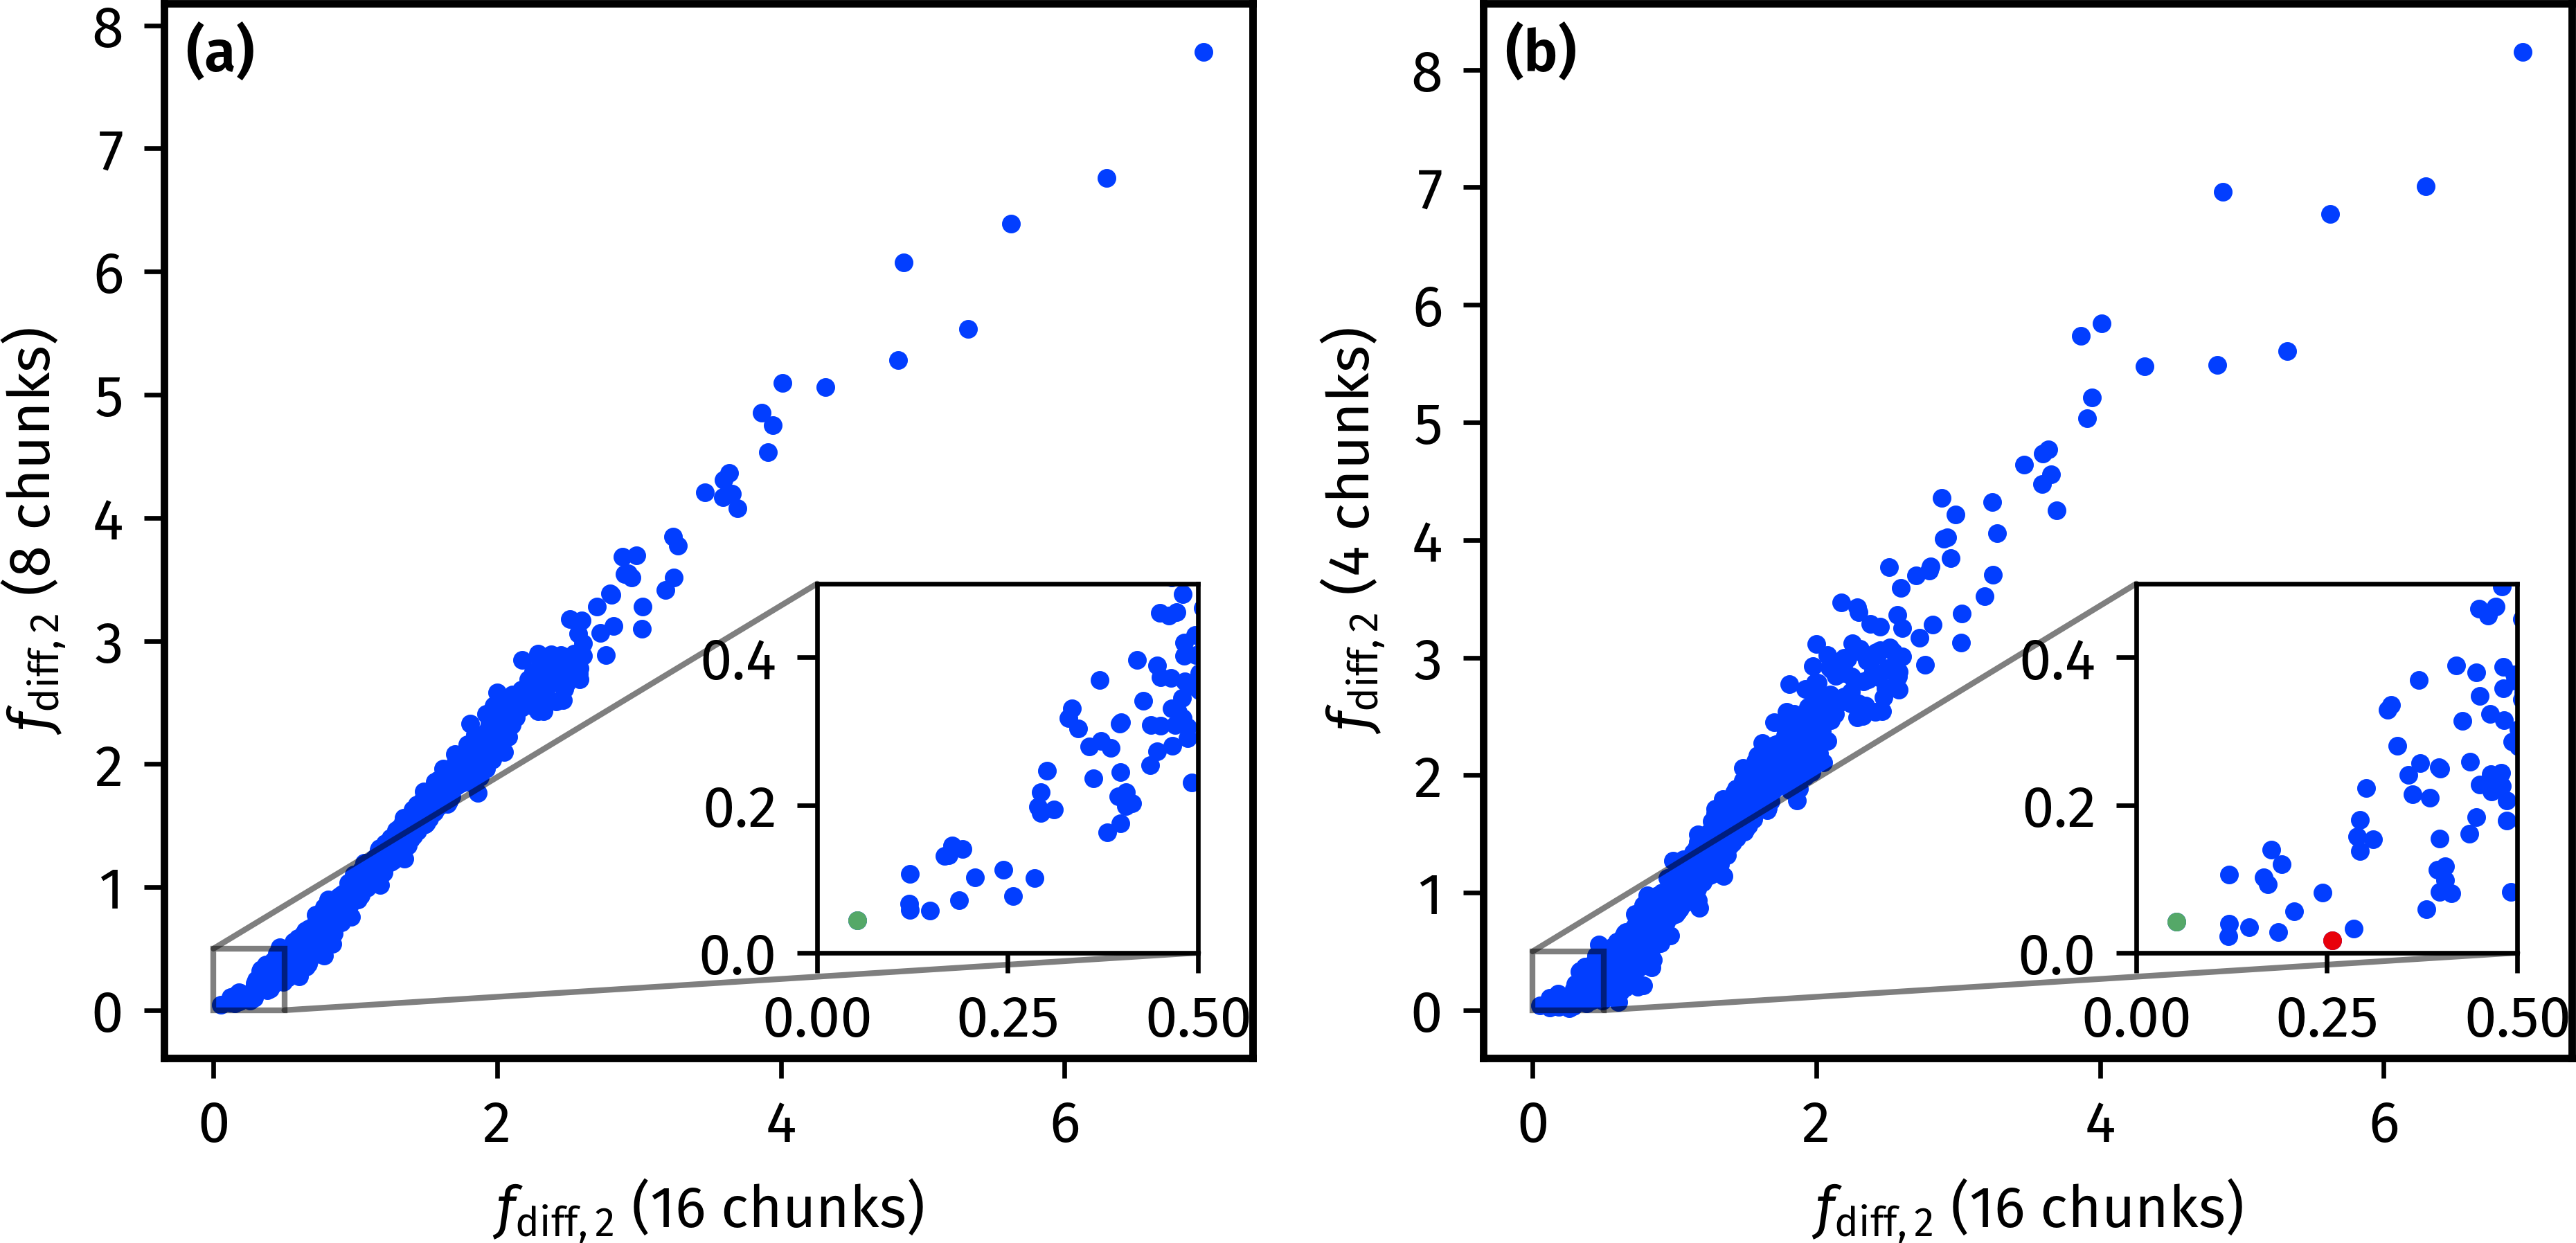
\includegraphics[]{pureshift/td1_cf.png}%
    {\phantomsubcaption\label{fig:dpsyche_td1_cf_16_8}}%
    {\phantomsubcaption\label{fig:dpsyche_td1_cf_16_4}}%
    \caption[Comparison of $f_\text{diff,2}$ cost function with different numbers of chunks]{
        Comparison of $f_\text{diff,2}$ values when simulated with different numbers of chunks.
        16 chunks is assumed to be the `gold standard'.
        \textbf{(\subref{fig:dpsyche_td1_cf_16_8})} Correlation between 16-chunk and 8-chunk cost functions.
        The `optimum' identified by both cost functions is plotted in green in the inset.
        \textbf{(\subref{fig:dpsyche_td1_cf_16_4})} Correlation between 16-chunk and 4-chunk cost functions.
        The `optima' identified by the 16- and 4-chunk cost functions are plotted in green and red respectively in the inset.
    }
    \label{fig:dpsyche_td1_cf}
\end{figure}

The 16-chunk and 8-chunk $f_\text{diff,2}$ (\cref{fig:dpsyche_td1_cf_16_8}) do in fact line up quite well.
Notably, as the inset shows, they both agree on the `best' candidate (note that this is not necessarily anywhere near perfect, since it was randomly generated).
The 4-chunk $f_\text{diff,2}$ also has the correct overall behaviour (\cref{fig:dpsyche_td1_cf_16_4}).
However, its ranking of the `best' candidates is not very accurate: the 4-chunk cost function rates the red dot in the inset as the optimum, but that is only the 13th-best candidate when using the 16-chunk cost function.
Ultimately, I decided to use the 4-chunk cost function for `quick and dirty' optimisations, where only an approximate optimum was required.
However, for anything requiring more accuracy, the 8-chunk cost function was used.

An optimisation was then carried out with a (rather arbitrarily chosen) setting of $m = 9$, i.e.\ nine hard pulses in the PSE.
A total of $s = 20$ spin systems were used, matching the number of CPU cores on the computer used for the optimisations: these were further subdivided into four two-spin systems, eight three-spin systems, and eight four-spin systems.
The derivative-based BFGS algorithm was used to carry out the optimisation: this is a popular line search algorithm which uses an approximate Hessian to calculate the search direction at each iteration.\autocite{Kelley1999,Nocedal2006}
No lower or upper bounds were placed on the flip angles or phases: phases can obviously simply be wrapped to the region $[0, 2\pi)$, and in the simulations, the hard pulses were modelled as being instantaneous rotations, so their flip angles can also just be wrapped to $[0, 2\pi)$.
(This would not be completely valid if realistic, finite pulses were used, since changing the flip angle would also change their duration.)
This first optimisation yielded the following optimised parameters for the nine pulses:
\begin{align}
    \{\beta_i\} &= \{\ang{118.6972}, \ang{29.8400}, \ang{107.4850}, \ang{190.4788}, \notag \\
                &\qquad \ang{138.4710}, \ang{144.5939}, \ang{18.9674}, \ang{73.8900}, \ang{130.6071}\} \label{eq:dpsyche_opt_nosens_angles} \\
     \{\phi_i\} &= \{\ang{144.5641}, \ang{173.3596}, \ang{38.9878}, \ang{146.3121}, \notag \\
                &\qquad \ang{127.7346}, \ang{7.5104}, \ang{36.9805}, \ang{110.2791}, \ang{182.3894}\}. \label{eq:dpsyche_opt_nosens_phases}
\end{align}
The fact that none of the flip angles exceeded \ang{360} here provides some justification for not using bounds in the optimisation.

\begin{figure}[htb]
    % I don't have the Matlab output data any more: it was done in
    % examples/run_opt_par() and predates some of the API rework to (e.g.)
    % enforce reproducibility. The angles and pulses are just taken from the
    % TopSpin data. :/ OK not ideal, I know, but too bad. Can't change it.
    % There IS one way to retrieve the data: rewind the entire git repo to this
    % date and rerun it.
    \centering
    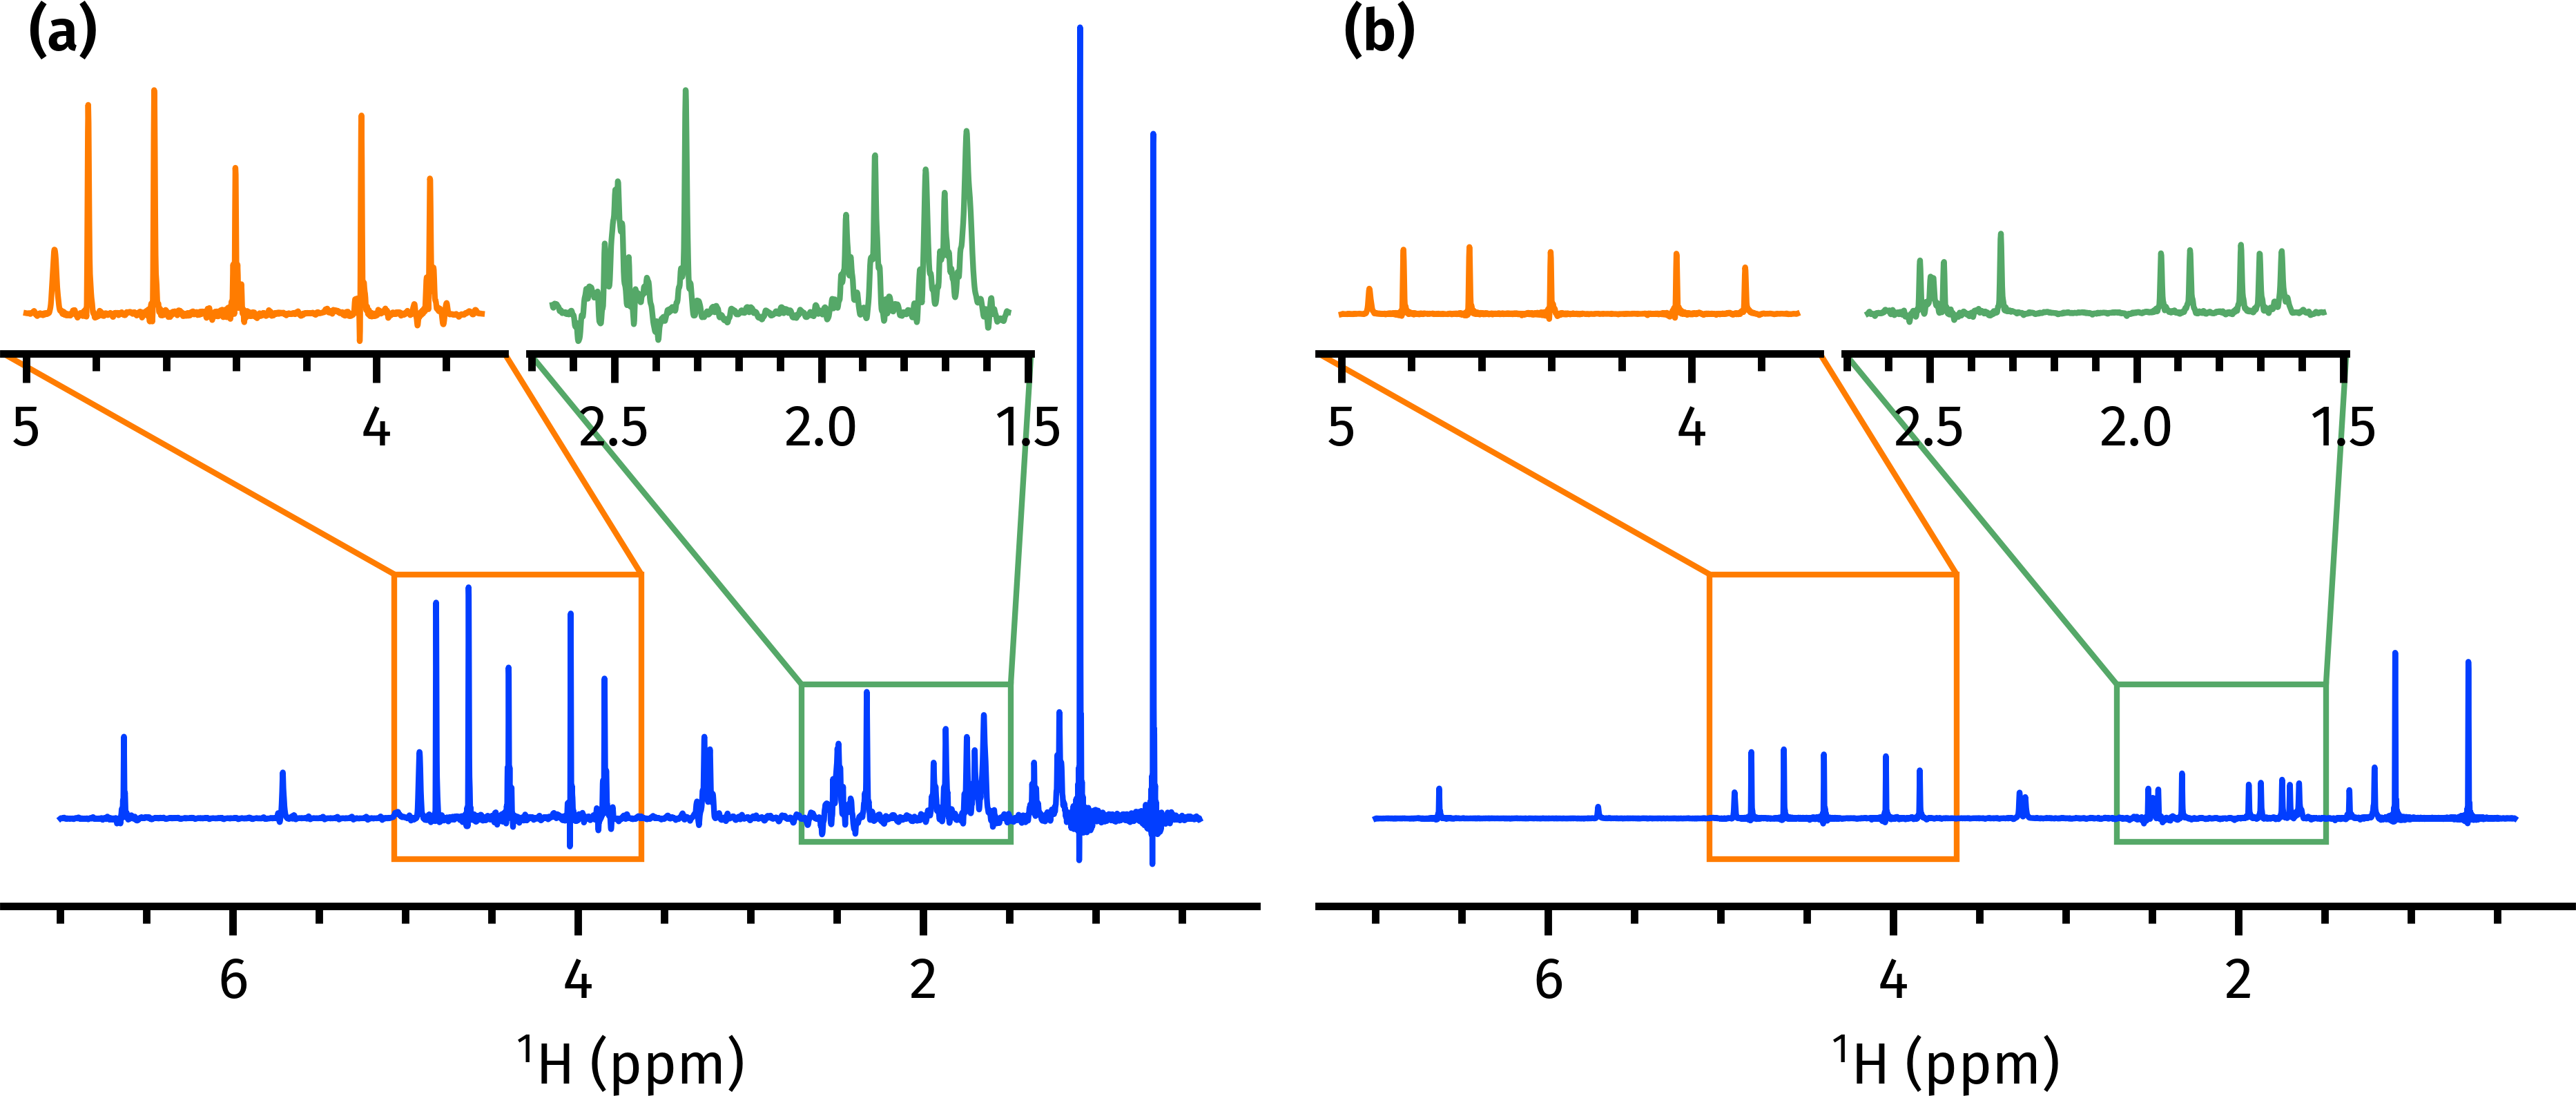
\includegraphics[]{pureshift/dpsyche_nosens_vs_psyche}%
    {\phantomsubcaption\label{fig:dpsyche_nosens_vs_psyche_dp}}%
    {\phantomsubcaption\label{fig:dpsyche_nosens_vs_psyche_p}}%
    \caption[Comparison of optimised dPSYCHE and PSYCHE]{
        \textbf{(\subref{fig:dpsyche_nosens_vs_psyche_dp})} dPSYCHE experiment acquired using the flip angles and phases in \cref{eq:dpsyche_opt_nosens_angles,eq:dpsyche_opt_nosens_phases}.
        The $\beta$ hard pulses in the PSE were applied with an RF amplitude of 
        \textbf{(\subref{fig:dpsyche_nosens_vs_psyche_p})} (Double-saltire) PSYCHE experiment acquired with $\beta = \ang{20}$.
        \datacode{6A-211027}
    }
    \label{fig:dpsyche_nosens_vs_psyche}
\end{figure}

To evaluate the quality of the decoupling on a real sample, the dPSYCHE experiment was performed experimentally, and the results compared against a PSYCHE experiment (\cref{fig:dpsyche_nosens_vs_psyche}).
Firstly, it is worth pointing out that a pure shift spectrum (even if not a very good one) was obtained: this validates the form of the PSE and the optimisation approach used here, especially considering that the optimisation was not tailored towards this particular sample.
The dPSYCHE experiment clearly has much greater sensitivity than the PSYCHE experiment; however, the decoupling quality is extremely poor.
The reason for this is likely because the optimisation is prioritising sensitivity too highly over purity, and ultimately stems from the factor $c$ in \cref{eq:f_diff_dpsyche} which we have ignored until now.
Since $c = 1$, the optimisation is essentially guiding the dPSYCHE experiment towards having \textit{exactly the same sensitivity as a pulse--acquire experiment}.

Although this might be a nice idea in principle, it is not physically sensible: no pure shift method has sensitivity which is even close to that of a pulse--acquire experiment.
It makes more sense to scale down the target spectrum by introducing a factor of $c < 1$ into the cost function (\cref{eq:f_diff_dpsyche}); the parameter $c$ therefore represents the `target sensitivity'.
By changing the parameter $c$, we can control whether the optimisation emphasises sensitivity or purity more.
(Note that this option was \textit{not} available to us in the experimental JRSE-based optimisations in \cref{sec:pureshift__optimisation}.)

A series of new optimisations were therefore run, with $c$ ranging from $0.2$ to $1$ (\cref{tbl:dpsyche_sens}).
The 4-chunk cost function was used, and the maximum number of function evaluations capped at 5000.
Each optimisation was run 10 times with a different starting seed, and the best of the 10 results chosen for further evaluation (\cref{tbl:dpsyche_sens}).
The resulting spectra (\cref{fig:dpsyche_sens}) show that adjusting $c$ has the desired effect: larger values lead to greater sensitivity and lower purity, and vice versa.

\begin{table}[htb]
    % matlab_nmr_jy/research/optim_specdiff/opt_sens.out
    \begin{tabular}{cccc}
        \toprule
        $c$ & \textbf{Flip angles} ($^\circ$) & \textbf{Phases} ($^\circ$) & $f_\text{diff,2}$ \\
        \midrule
        1 & \makecell{59.8813, 96.0748, 111.5862, \\ 118.7285, 144.701, 176.9773, \\ 29.2866, 40.0658, 63.8237} & \makecell{355.773, 81.741, 99.8752, \\ 81.6675, 337.0056, 150.7004, \\ 105.9666, 317.9979, 27.7897} & 0.0404 \\
        \midrule
        0.8 & \makecell{81.9461, 65.311, 90.3488, \\ 106.6388, 73.3462, 196.7857, \\ 51.791, 34.8188, 53.9506} & \makecell{329.8571, 60.3564, 137.3929, \\ 68.5286, 340.74, 126.29, \\ 64.4601, 145.4714, 27.3019} & 0.0321 \\
        \midrule
        0.6 & \makecell{53.1313, 82.2547, 88.6093, \\ 161.9291, 83.462, 161.3548, \\ 14.2976, 66.2199, 53.9709} & \makecell{347.2835, 59.5518, 68.072, \\ 113.5358, 34.5537, 156.191, \\ 268.7641, 302.7427, 16.29} & 0.0250 \\
        \midrule
        0.4 & \makecell{77.2998, 127.7274, 87.6663, \\ 104.6371, 99.6474, 168.8171, \\ 8.8569, 52.7865, 58.1408} & \makecell{342.2787, 47.7526, 76.4114, \\ 97.3304, 14.2178, 163.9513, \\ 94.2575, 280.0273, 16.0971} & 0.0271 \\
        \midrule
        0.2 & \makecell{120.6613, 107.6712, 84.0427, \\ 133.5377, 82.1999, 223.122, \\ 41.1617, 41.9398, 12.016} & \makecell{347.2051, 79.4503, 109.8796, \\ 83.5017, 345.4284, 133.8355, \\ 66.4118, 201.0041, 4.4419} & 0.0261 \\
        \midrule
        0.4* & \makecell{92.4395, 133.2136, 38.9704, \\ 34.9182, 56.0256, 57.4097, \\ 31.5916, 140.1088, 128.7125} & \makecell{62.036, 16.411, 319.5634, \\ 128.4443, 49.7357, 328.5103, \\ 210.6498, 44.0123, 327.4517} & 0.0108 \\
        \bottomrule
    \end{tabular}
    \caption[dPSYCHE optimisation results for different sensitivities]{
        Results of dPSYCHE optimisations for different sensitivities.
        Note that since the cost function depends on the value of $c$, the exact value of $f_\text{diff,2}$ for these optimisations cannot be compared to one another; they are only presented here for completeness.
        The final entry, labelled with an asterisk, was run with no limit on the number of function evaluations (this is discussed further in the text).
    }
    \label{tbl:dpsyche_sens}
\end{table}

\begin{figure}[htbp]
    % matlab_nmr_jy/research/optim_specdiff/opt_sens.m
    \centering
    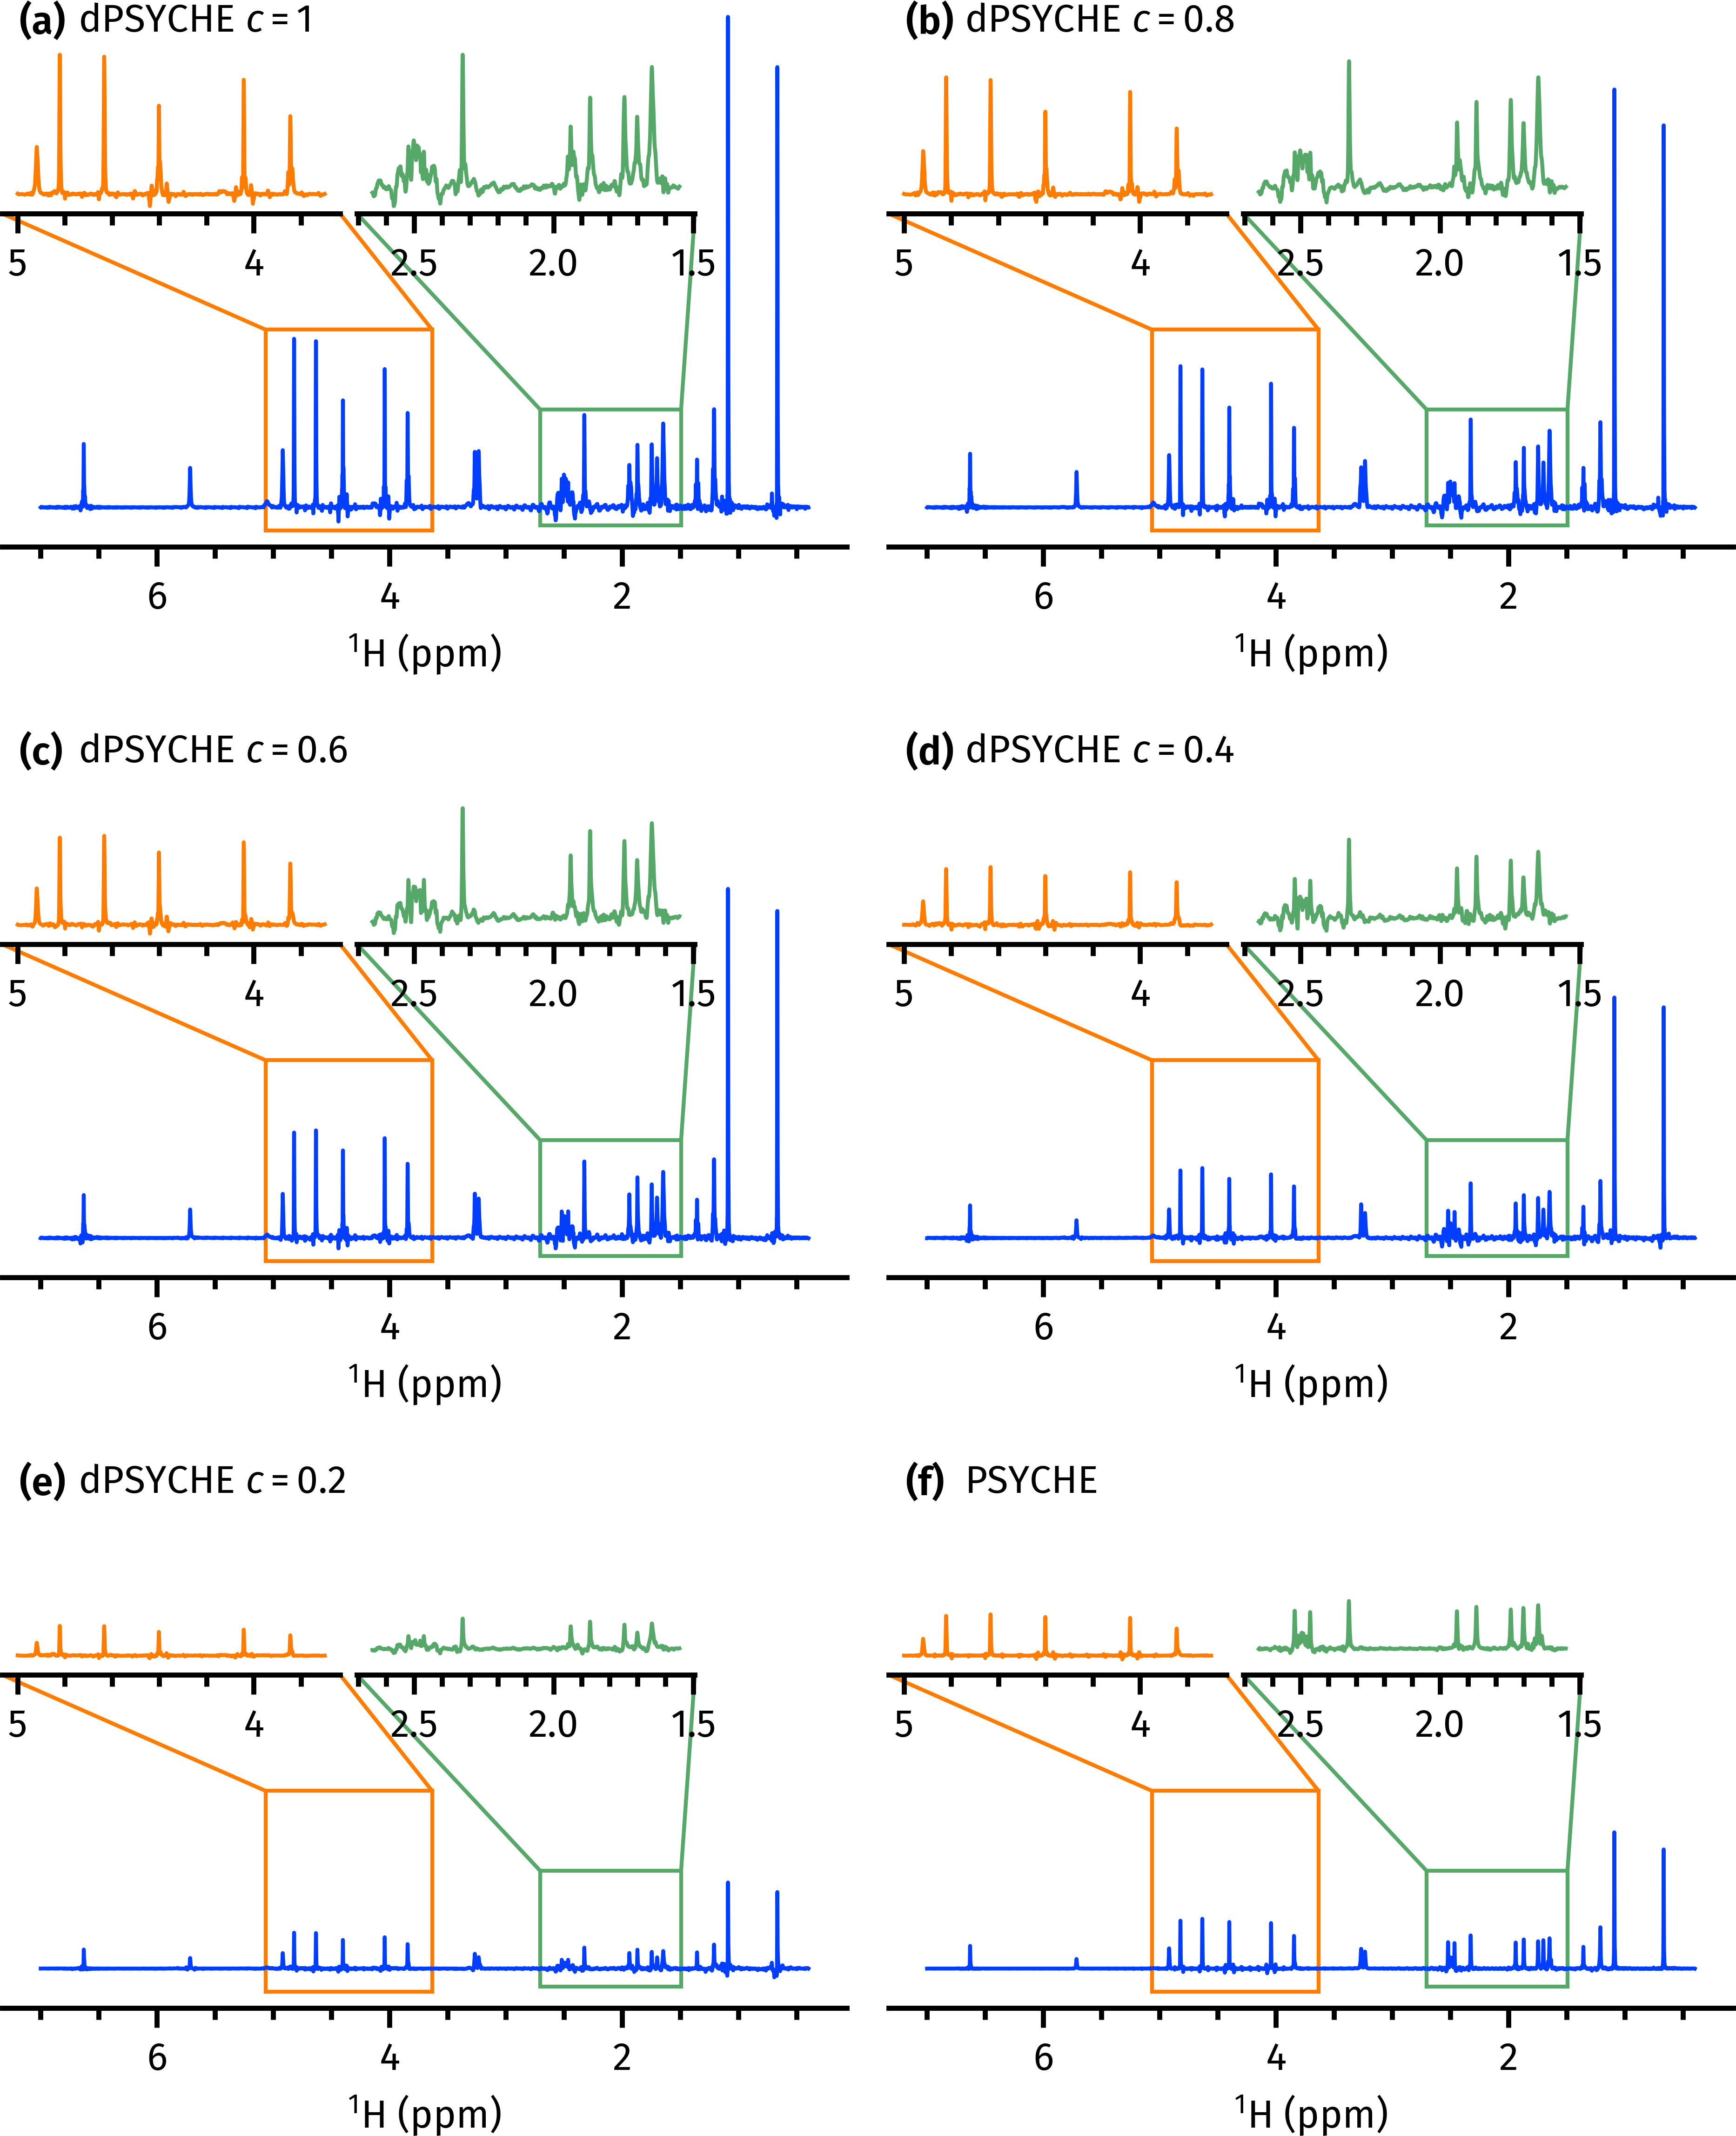
\includegraphics[]{pureshift/dpsyche_sens.png}%
    {\phantomsubcaption\label{fig:dpsyche_sens_d1}}%
    {\phantomsubcaption\label{fig:dpsyche_sens_d0p8}}%
    {\phantomsubcaption\label{fig:dpsyche_sens_d0p6}}%
    {\phantomsubcaption\label{fig:dpsyche_sens_d0p4}}%
    {\phantomsubcaption\label{fig:dpsyche_sens_d0p2}}%
    {\phantomsubcaption\label{fig:dpsyche_sens_p}}%
    \caption[dPSYCHE optimisations with different sensitivities]{
        \textbf{(\subref{fig:dpsyche_sens_d1})} dPSYCHE, $c = 1$.
        \textbf{(\subref{fig:dpsyche_sens_d0p8})} dPSYCHE, $c = 0.8$.
        \textbf{(\subref{fig:dpsyche_sens_d0p6})} dPSYCHE, $c = 0.6$.
        \textbf{(\subref{fig:dpsyche_sens_d0p4})} dPSYCHE, $c = 0.4$.
        \textbf{(\subref{fig:dpsyche_sens_d0p2})} dPSYCHE, $c = 0.2$.
        \textbf{(\subref{fig:dpsyche_sens_p})} Double-saltire PSYCHE with $\beta = \ang{20}$.
        All spectra and insets are plotted to scale to allow for sensitivity comparisons.
        \datacode{6A-211231}
    }
    \label{fig:dpsyche_sens}
\end{figure}

In this spectrum of andrographolide, the \qtyrange{3.5}{5}{\ppm} region (blue inset) is an `easier' region to decouple: there are fewer couplings here and all spin systems are firmly within the weak coupling regime.
The \qtyrange{1.5}{2.8}{\ppm} region (orange inset) is `more difficult' to decouple, especially the two peaks at \qty{2.5}{\ppm}, which are mutually strongly coupled.
The dPSYCHE spectrum with $c = 0.4$ appeared to be a good compromise between purity and sensitivity: its sensitivity was higher than that of the original (\ang{20} flip angle) PSYCHE experiment.
Furthermore, it provided good decoupling in the `easier' deshielded region and somewhat acceptable performance in the shielded region, with the notable exception of the strongly coupled peaks at \qty{2.5}{\ppm}.

I therefore ran a longer optimisation using the same starting point and with no limit on the number of function evaluations, which successfully lowered the cost function value by twofold (the last entry in \cref{tbl:dpsyche_sens}).
The pure shift spectrum obtained using these optimised pulses is shown in \cref{fig:dpsyche_optsens3}.
The decoupling quality in both regions is comparable to that in the PSYCHE spectrum, again with the exception of the strongly coupled peaks at \qty{2.5}{\ppm}.

\begin{figure}[htb]
    % matlab_nmr_jy/research/optim_specdiff/opt_sens3.m
    \centering
    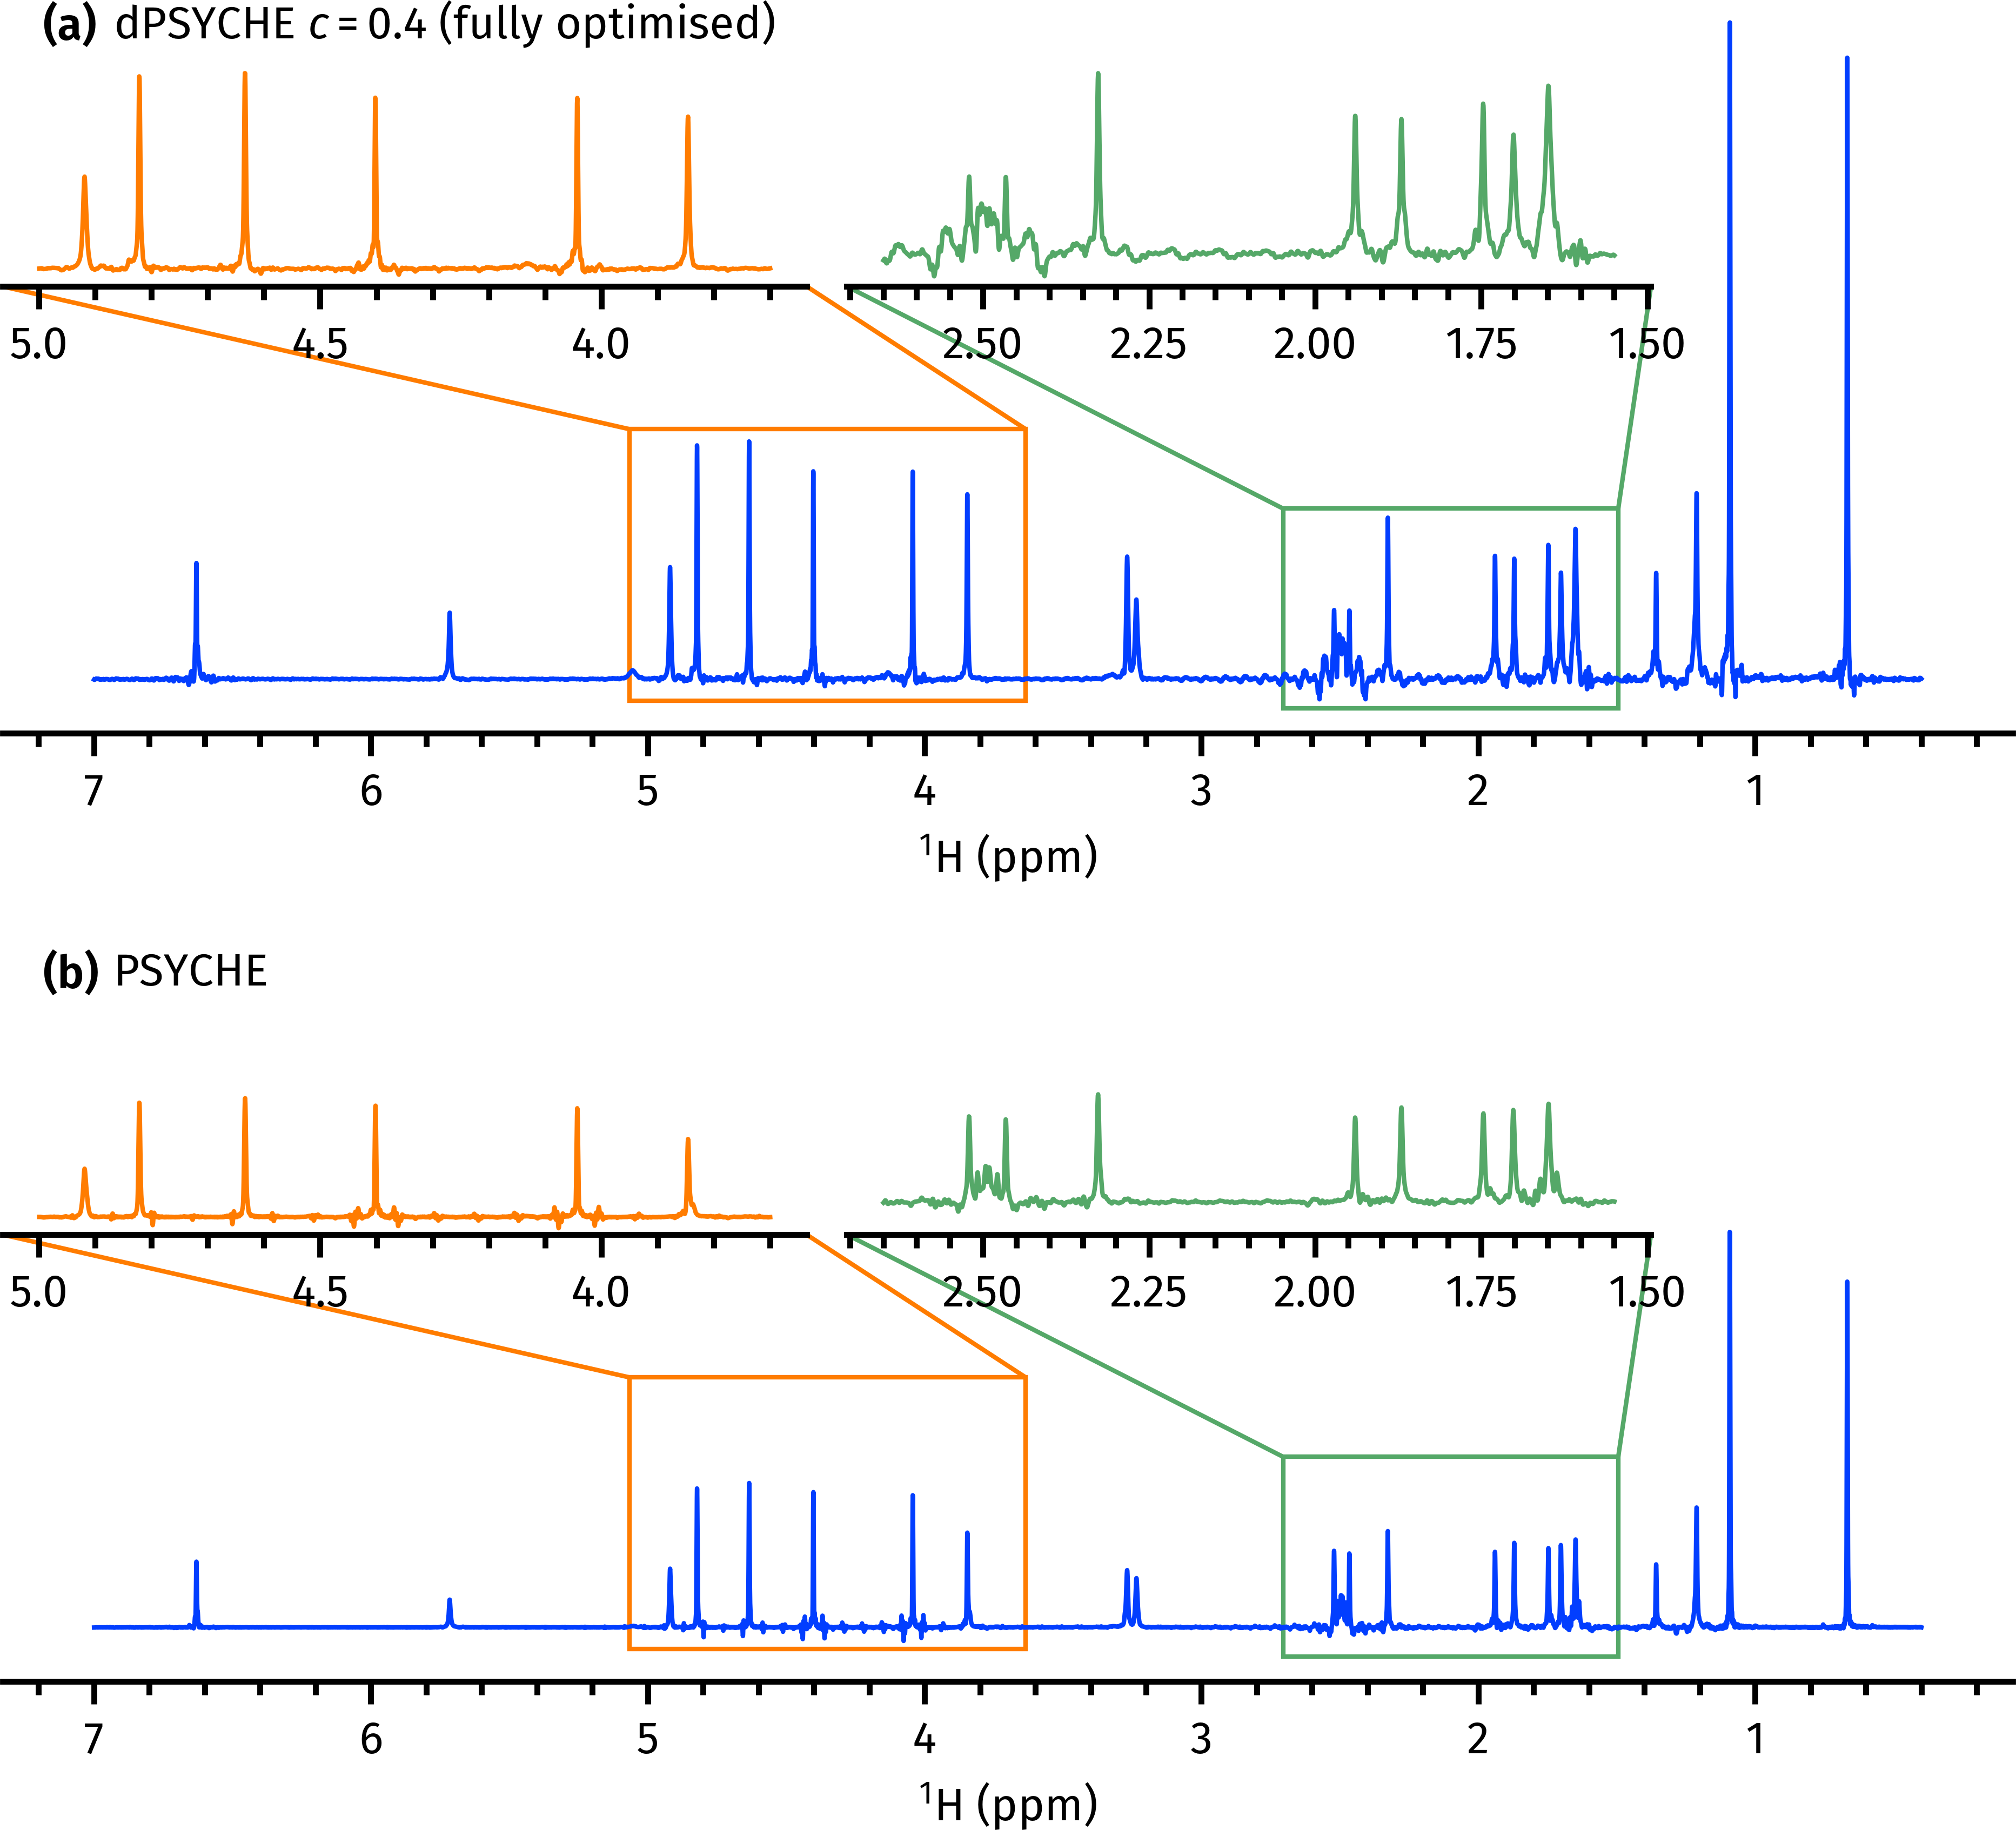
\includegraphics[]{pureshift/dpsyche_optsens3.png}%
    {\phantomsubcaption\label{fig:dpsyche_optsens3_d}}%
    {\phantomsubcaption\label{fig:dpsyche_optsens3_p}}%
    \caption[dPSYCHE final optimisation with $c = 0.4$]{
        \textbf{(\subref{fig:dpsyche_optsens3_d})} Fully optimised dPSYCHE experiment with $c = 0.4$.
        \textbf{(\subref{fig:dpsyche_optsens3_p})} Double-saltire PSYCHE with $\beta = \ang{20}$.
        \datacode{6A-211231}
    }
    \label{fig:dpsyche_optsens3}
\end{figure}

\begin{figure}[htb]
    % matlab_nmr_jy/research/optim_specdiff/opt_sens3.m but with different pulprog
    \centering
    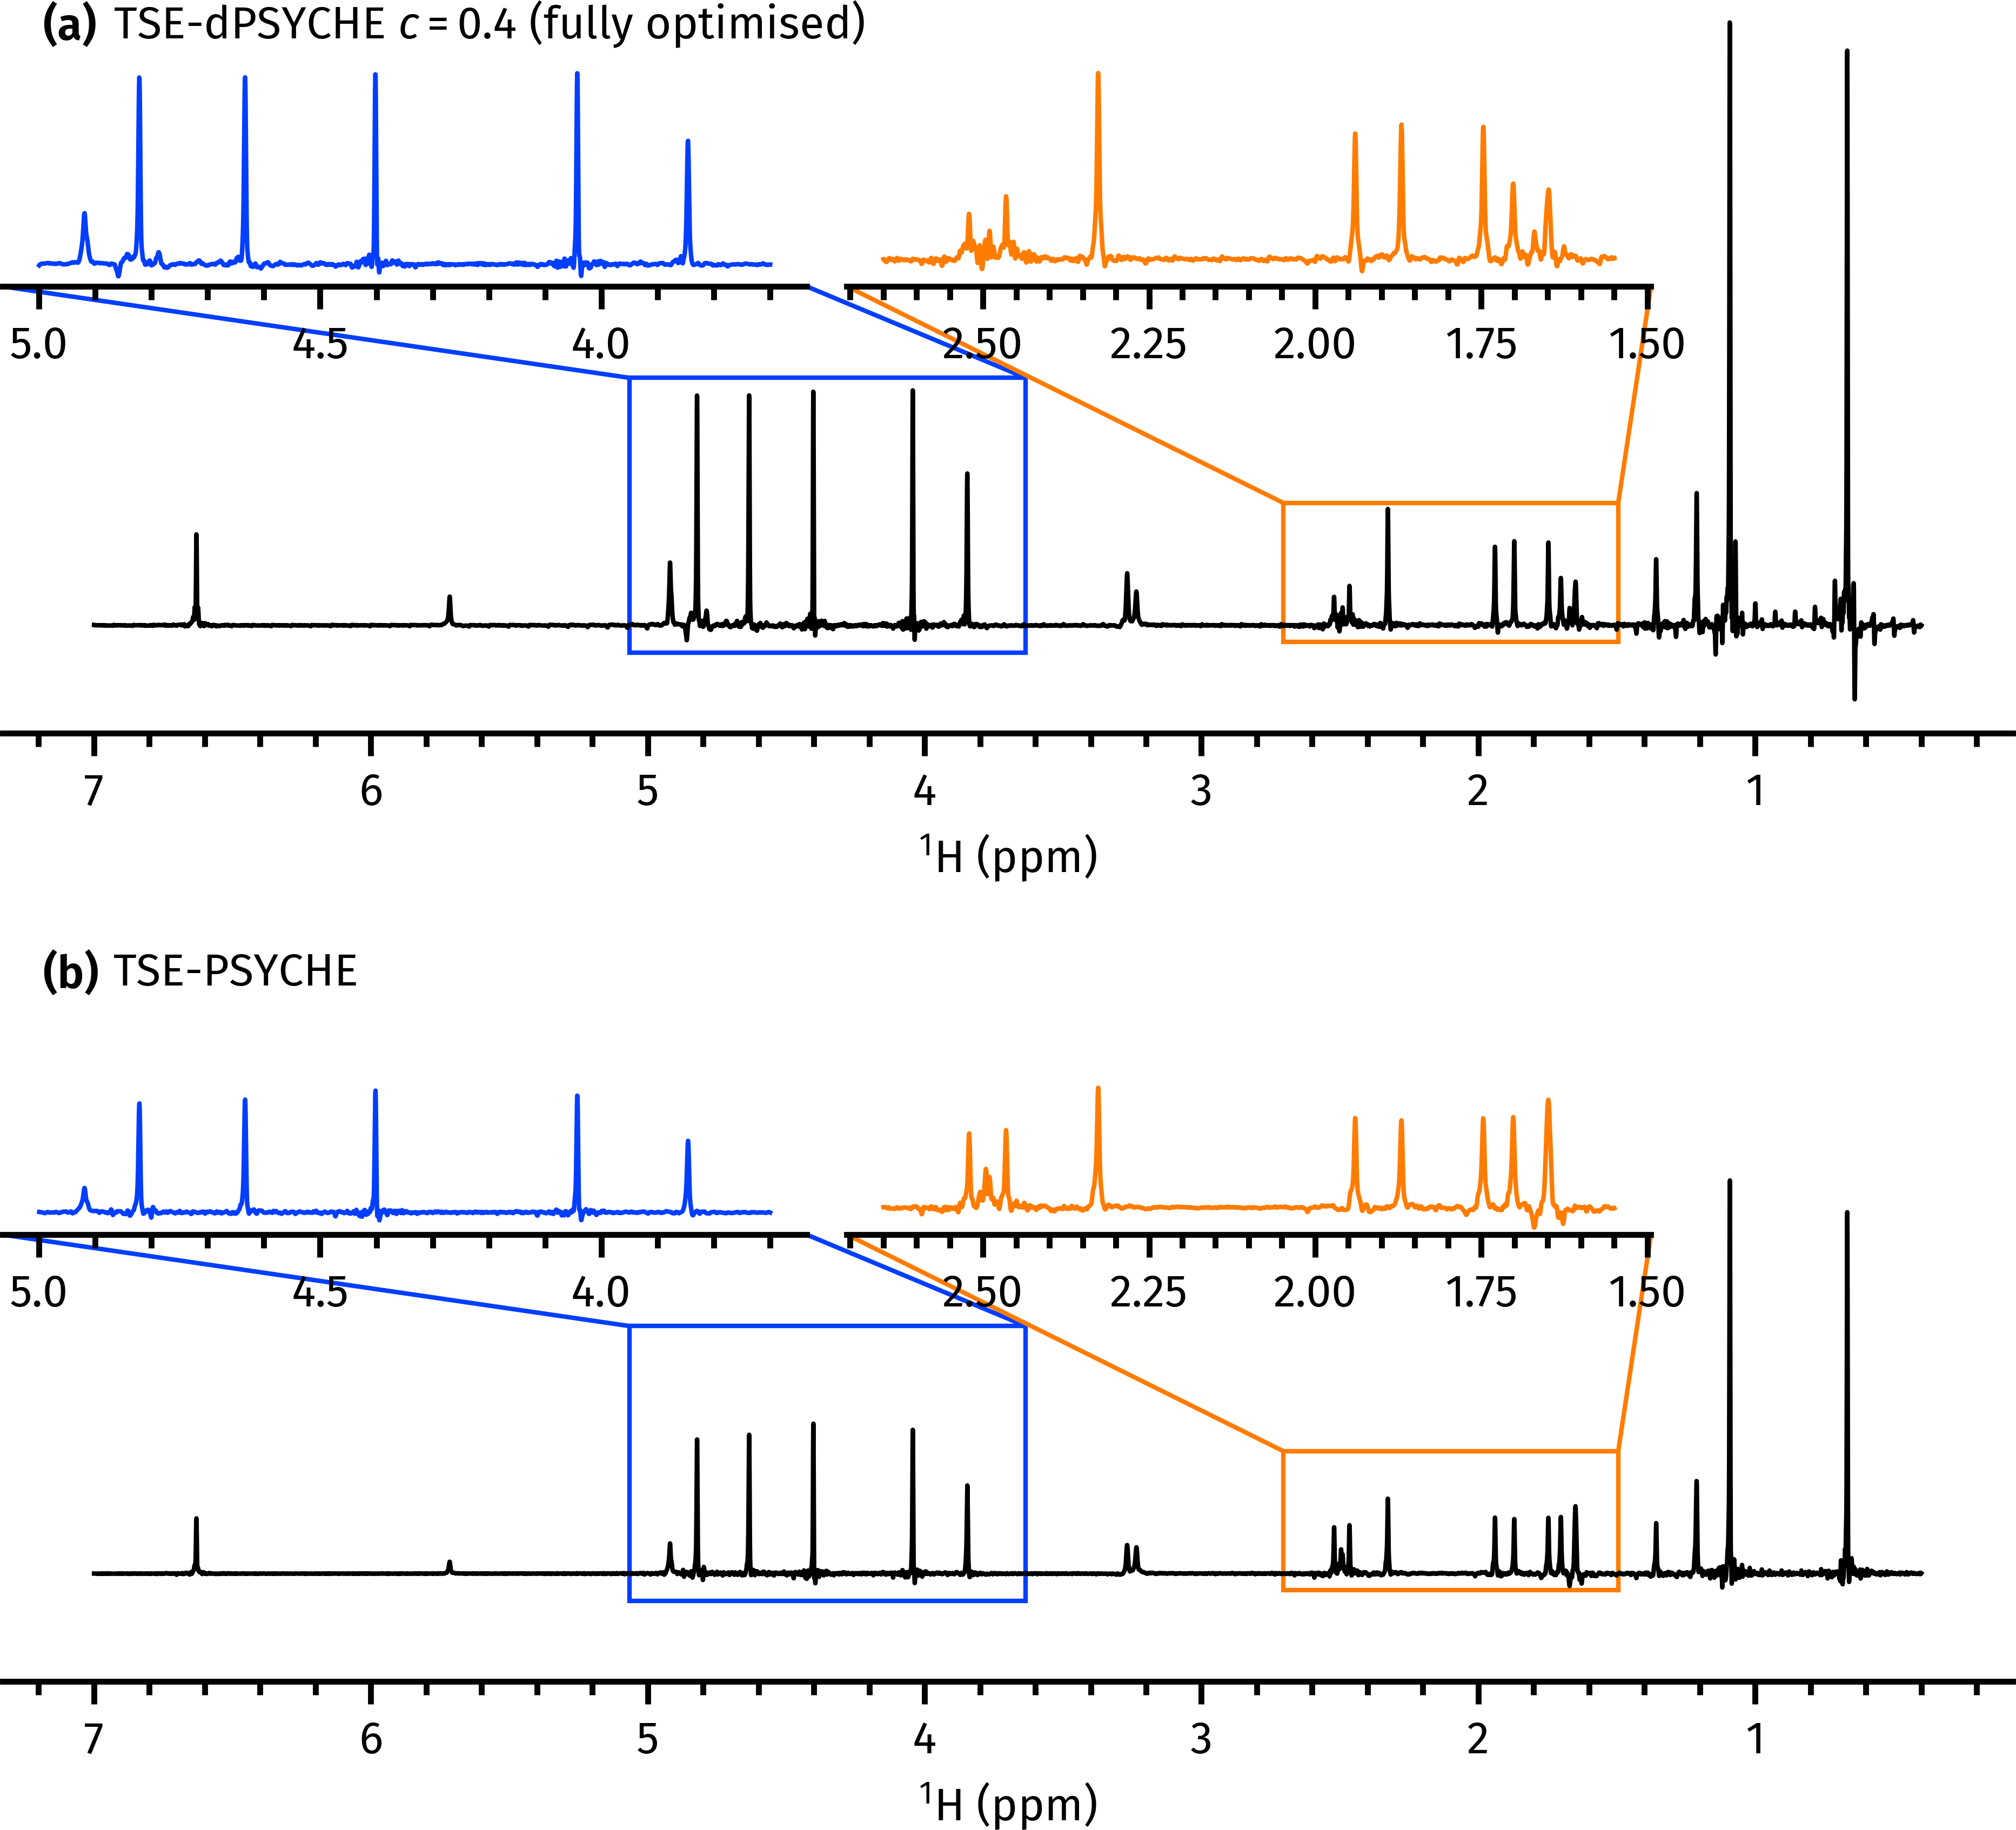
\includegraphics[]{pureshift/tsedpsyche_optsens3.png}%
    {\phantomsubcaption\label{fig:tsedpsyche_optsens3_d}}%
    {\phantomsubcaption\label{fig:tsedpsyche_optsens3_p}}%
    \caption[TSE-dPSYCHE final optimisation with $c = 0.4$]{
        \textbf{(\subref{fig:tsedpsyche_optsens3_d})} Fully optimised TSE-dPSYCHE experiment with $c = 0.4$.
        \textbf{(\subref{fig:tsedpsyche_optsens3_p})} Double-saltire TSE-PSYCHE with $\beta = \ang{20}$.
        \datacode{7A-220129}
    }
    \label{fig:tsedpsyche_optsens3}
\end{figure}

To make the dPSYCHE experiment more robust towards strong coupling, a TSE version of the sequence was also written and tested (\cref{fig:tsedpsyche_optsens3}).
This did indeed improve the decoupling at \qty{2.5}{\ppm}, as expected.
However, although the TSE-dPSYCHE version still retains its \textit{overall} sensitivity advantage over TSE-PSYCHE (especially evident in the deshielded region), this is not true of every peak: the two peaks at 1.65 and \qty{1.70}{\ppm} seem to have decreased intensities in the TSE-dPSYCHE experiment.
The reason for this remains unclear.

% number of pulses (maybe can omit?)
\iffalse
I then ran several preliminary screens to decide on the number of pulses to include in the pulse sequence.
Here, the 8-chunk cost function was used.
To save time, the total number of function evaluations was capped at 600 times the number of pulses: this, together with the fact that only one optimisation per category was run, means that these results are more suggestive rather than conclusive.
(Since the BFGS algorithm is a local optimiser, and the trajectory depends quite strongly on the initial point, the optimisation should \textit{in theory} be run with several different initial points.)
There was no clear winner, but the optimisations with 9 and 15 pulses yielded the best results; since optimising 18 parameters is easier than 30, I opted to go with 9 pulses.

\begin{figure}[htb]
    \centering
    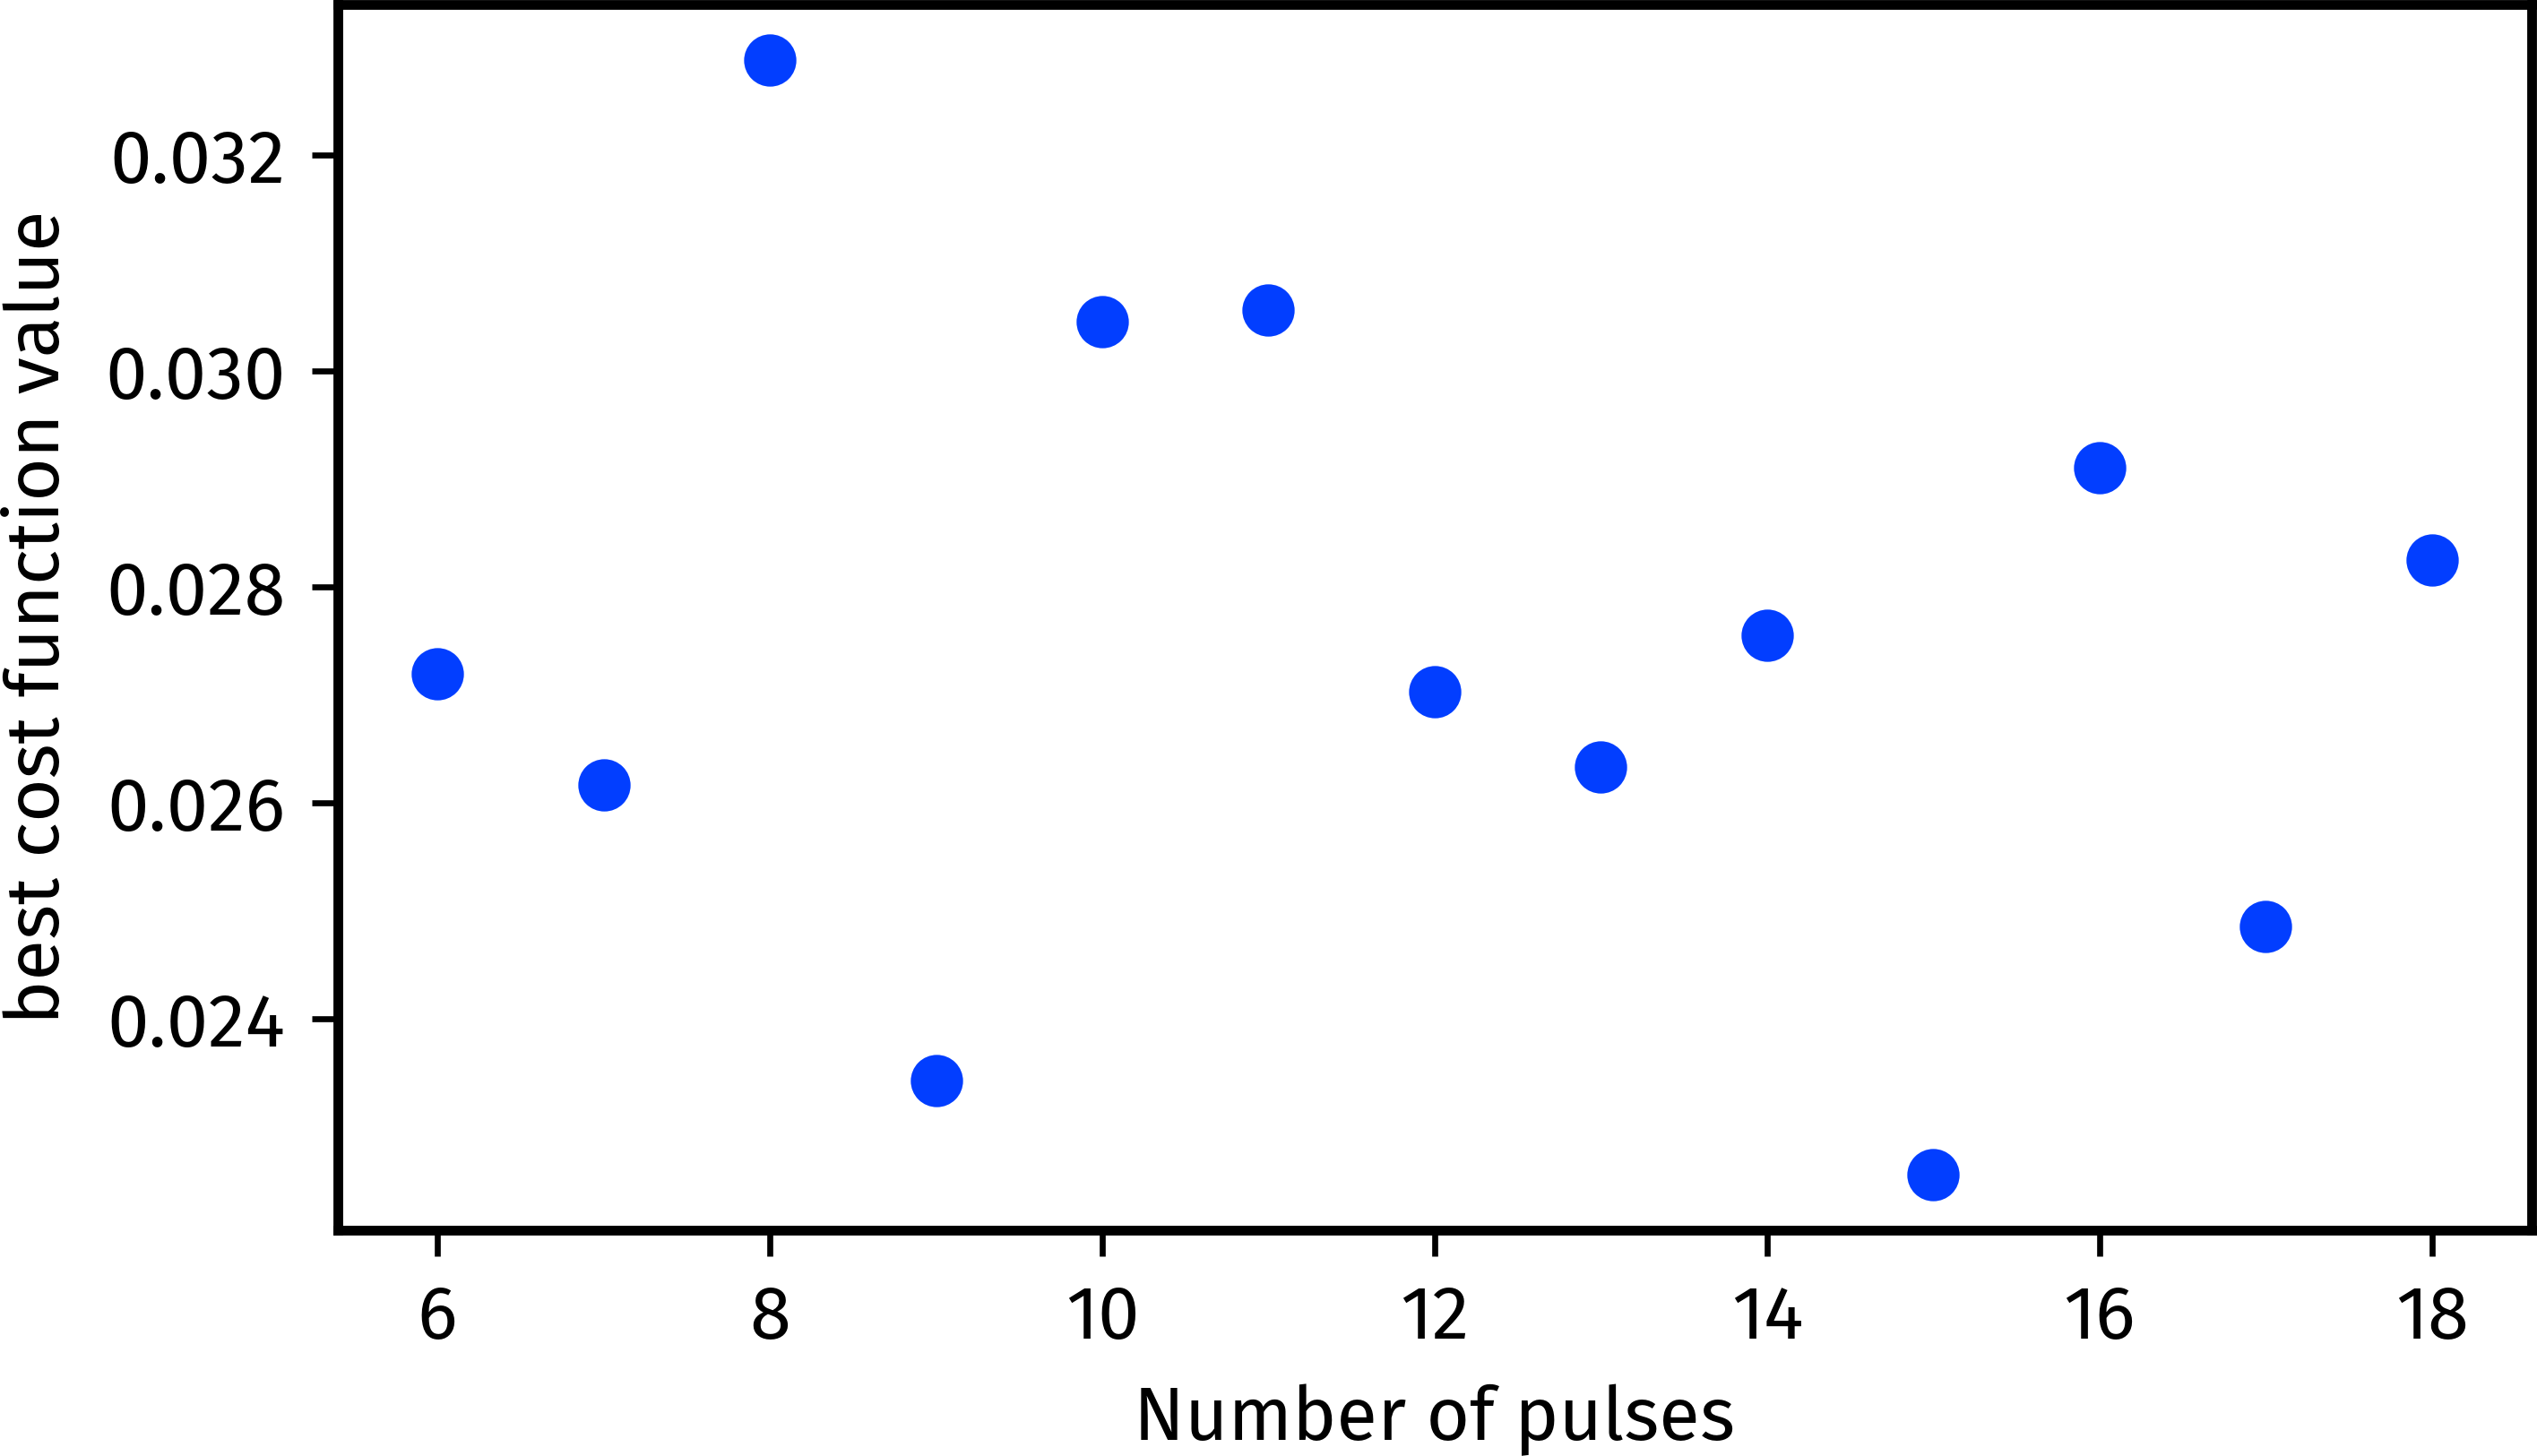
\includegraphics[]{pureshift/opt_npulses.png}%
    \caption[Comparison of cost functions attained with different numbers of pulses]{Blah}
    \label{fig:dpsyche_opt_npulses}
\end{figure}
\fi

\todo{State optimisation?}

% state optimisation

% conclusions and future work


\section{Ultrafast PSYCHE-iDOSY}
\label{sec:pureshift__epsidosy}

In the final section of this chapter, I turn to something entirely different: the combination of pure shift diffusion NMR with ultrafast acquisition.
This work was done in collaboration with Jean-Nicolas Dumez (University of Nantes): the original project idea was first conceived and implemented there.
Unfortunately, the results we obtained at Oxford were not promising enough to drive the project further, especially in light of time constraints.
However, for the sake of completeness, I describe the overall concept as well as these results in this section.

\begin{figure}[htb]
    \centering
    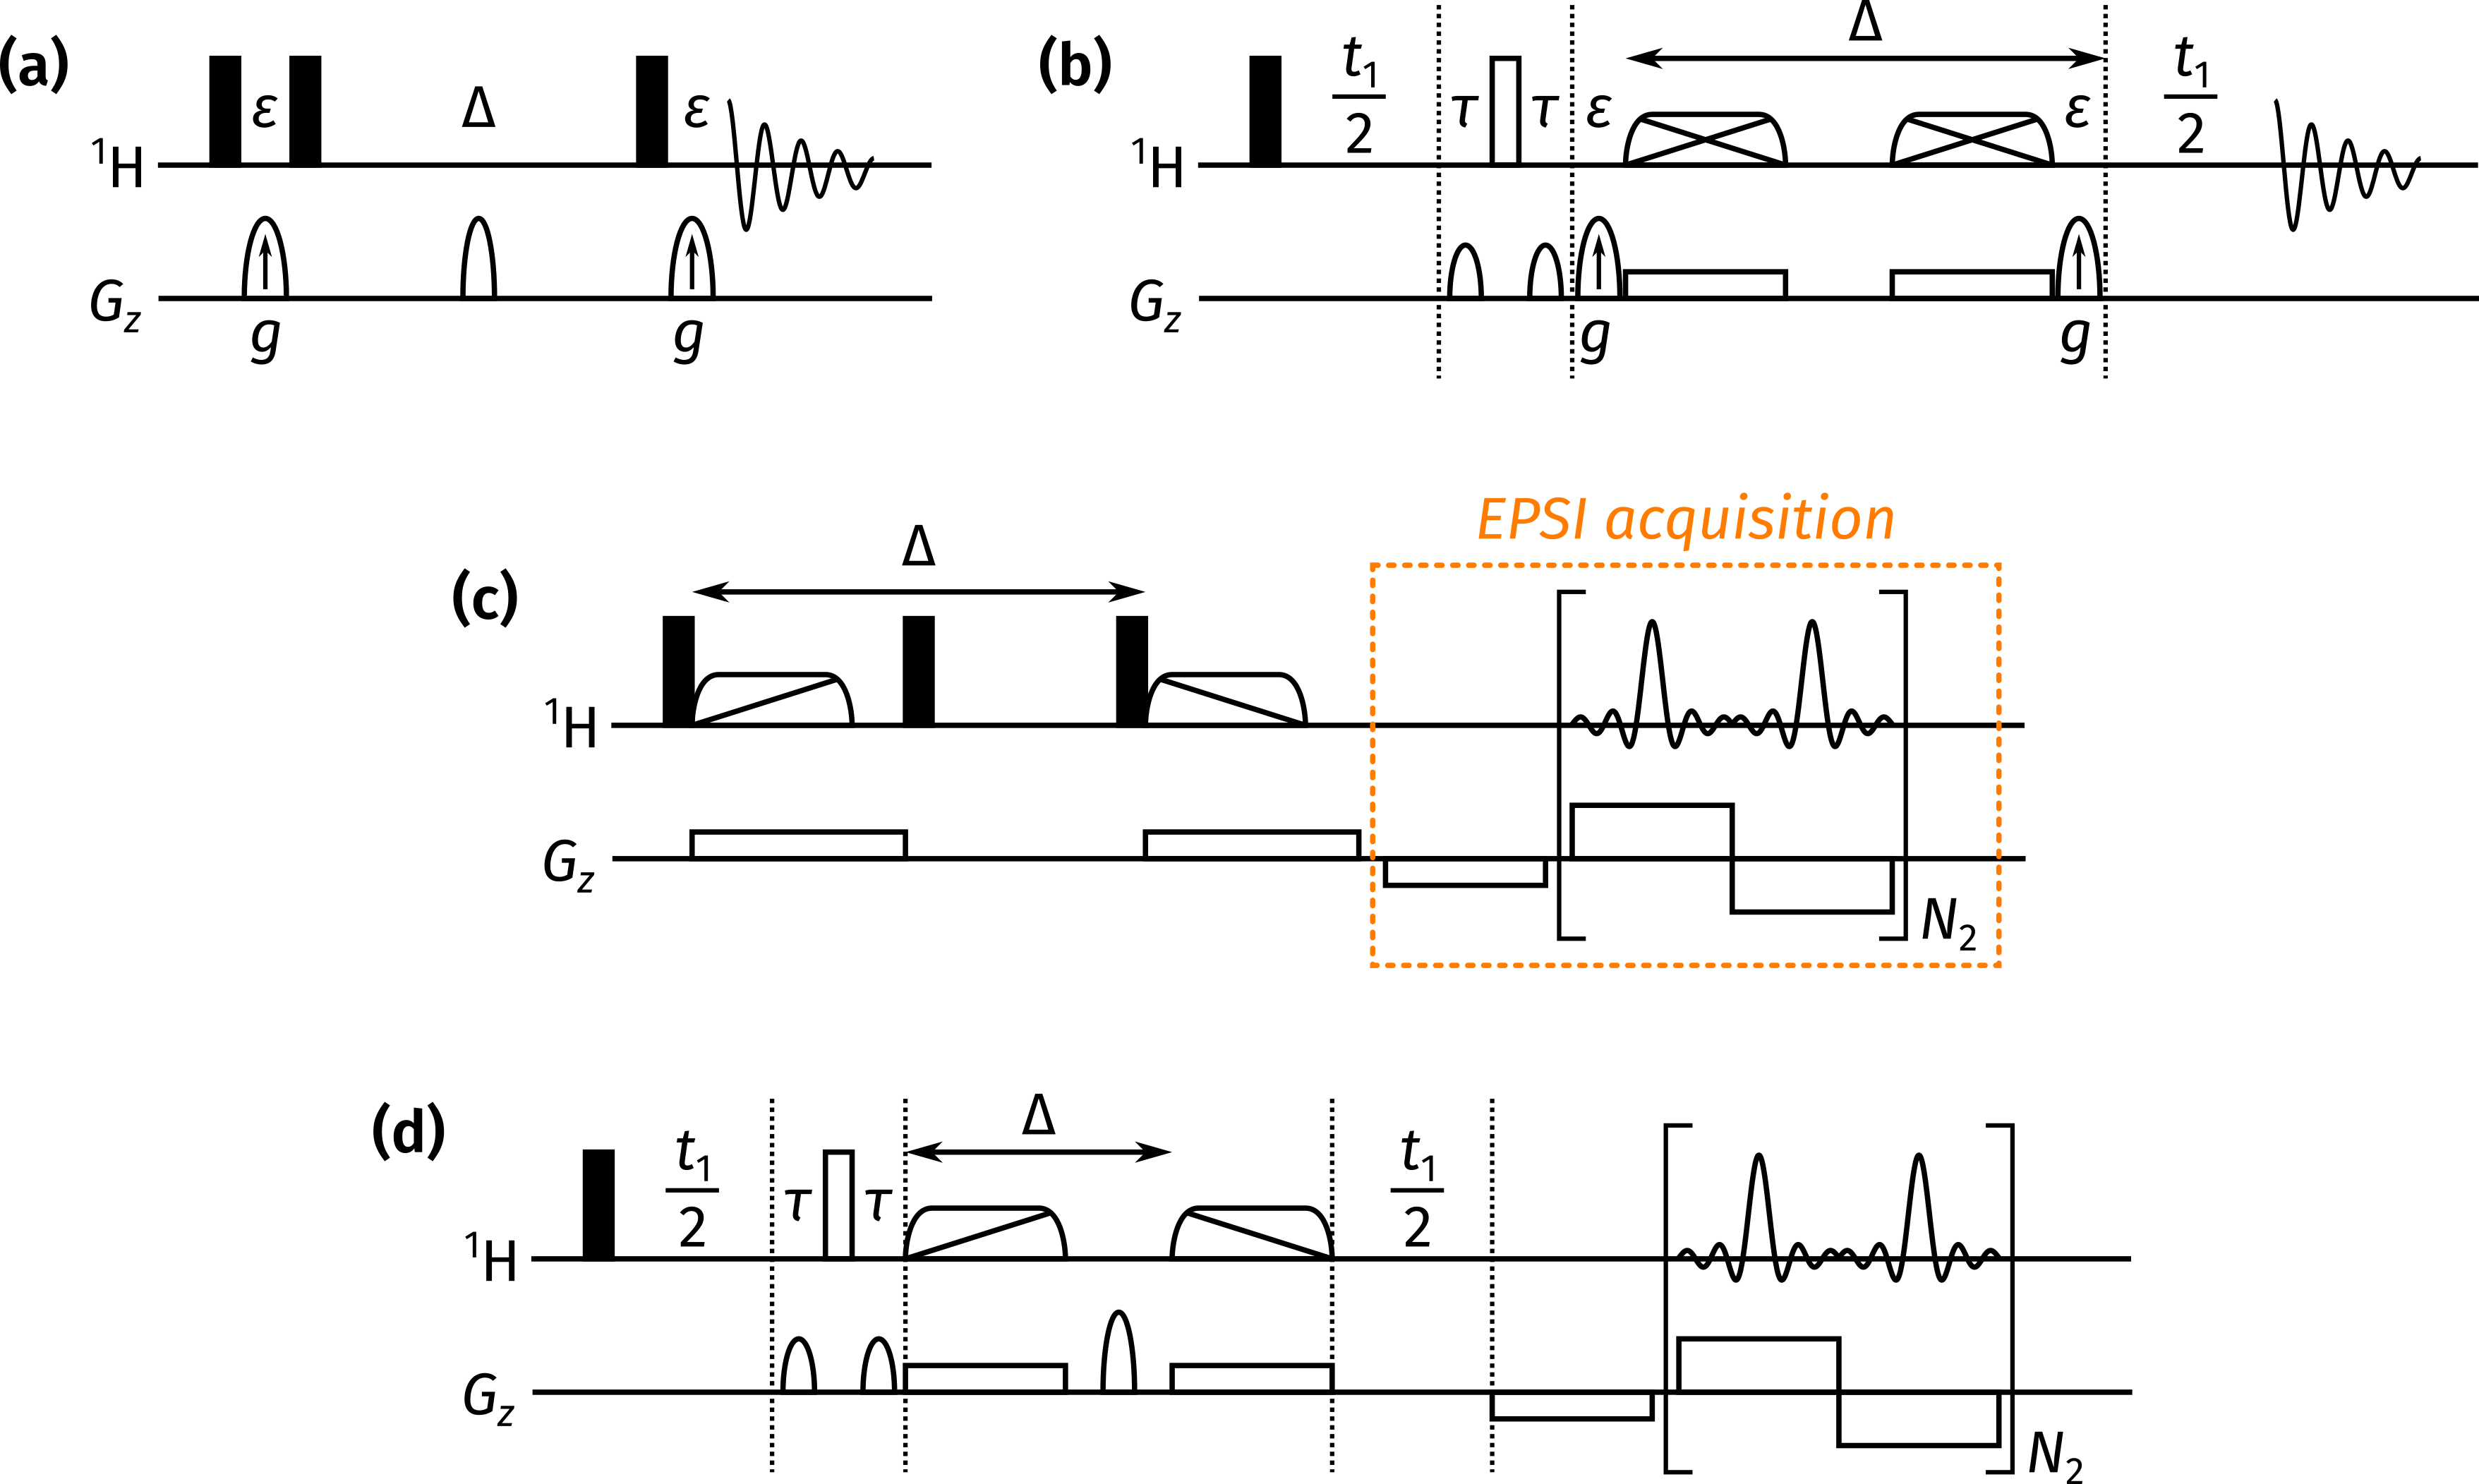
\includegraphics[]{pp/pureshift/epd_pulseq.png}%
    {\phantomsubcaption\label{fig:epd_pulseq_stedosy}}%
    {\phantomsubcaption\label{fig:epd_pulseq_psychedosy}}%
    {\phantomsubcaption\label{fig:epd_pulseq_epsidosy}}%
    {\phantomsubcaption\label{fig:epd_pulseq_epsipsychedosy}}%
    \caption[EPSI PSYCHE-iDOSY and associated pulse sequences]{
        \textbf{(\subref{fig:epd_pulseq_stedosy})} Basic stimulated echo DOSY experiment.
        To acquire the diffusion dimension, the amplitudes of gradients with arrows inside are incremented.
        $\Delta$ indicates the diffusion delay.
        \textbf{(\subref{fig:epd_pulseq_psychedosy})} PSYCHE-iDOSY experiment. $\tau$ is set to $1/(4 \cdot T_\text{chunk})$, as before.
        \textbf{(\subref{fig:epd_pulseq_epsidosy})} Ultrafast DOSY experiment. The EPSI acquisition block is highlighted in orange, consisting of a prephasing gradient followed by detection in the presence of alternating gradients.
        \textbf{(\subref{fig:epd_pulseq_epsipsychedosy})} Ultrafast PSYCHE-iDOSY experiment. Note the use of unidirectional chirps rather than saltire pulses.
    }
    \label{fig:epd_pulseq}
\end{figure}

Diffusion NMR\autocite{Johnson1999PNMRS} is covered in more detail in \cref{subsec:poise__diffusion}; however, I provide a brief overview of it here.
\Cref{fig:epd_pulseq_stedosy} shows a typical 2D stimulated echo DOSY experiment, where the indirect (diffusion) dimension involves the incrementation of gradient amplitudes rather than an evolution delay.
For each gradient amplitude, one time-domain signal is recorded.
Molecular diffusion during a delay placed between a pair of gradients leads to attenuation of the signal, as the spatially-dependent phase imparted by the first gradient is not perfectly refocused by the second.
This attenuation is described by the Stejskal--Tanner equation\autocite{Stejskal1965JCP,Sinnaeve2012CMR}, which in its simplest form is:
\begin{equation}
    \label{eq:stejskal_tanner}
    I(G) = I(0) \exp\left[-(\gamma\delta G)^2 D \Delta'\right].
\end{equation}
Here, $I(G)$ represents the signal intensity when measured with a gradient amplitude of $G$; $\gamma$ is the magnetogyric ratio, $\delta$ is the duration of the bracketing gradients, $D$ the diffusion coefficient, and $\Delta'$ a `corrected' diffusion delay.
The exact correction required depends on the shapes of the gradients used.
By measuring the signal intensity $I$ for at least two different values of $G$, the diffusion coefficient $D$ can be estimated.%
\footnote{As will be discussed in \cref{subsec:poise__diffusion}, this should really be an \textit{apparent} diffusion coefficient as there are various other factors which can affect the intensity, notably convection.}

The fact that different molecules have different diffusion coefficients, and thus different attenuation profiles, can be used to separate mixtures of molecules through the basic DOSY experiment.
However, when signals from different species overlap in the \proton{} spectrum, (as is often the case in mixtures), it is not possible to cleanly extract the separate peak intensities, resulting in poor resolution in the diffusion dimension.
There are several ways to solve this issue: for example, peaks can be resolved using another chemical shift dimension in a 3D experiment.\autociteset{3ddosy}
A slightly less time-consuming option is pure shift NMR.
The first pure shift diffusion experiments used either the \ang{45} projection of a 2DJ spectrum\autocite{Cobas2004JMR}, or the Zangger--Sterk PSE\autocite{Nilsson2007CC,Aguilar2010ACIE,Glanzer2014CEJ}: in both cases, improvements in the resolution of diffusion coefficients were reported.
The PSYCHE-iDOSY experiment\autocite{Foroozandeh2016ACIE} (\cref{fig:epd_pulseq_psychedosy}) improved upon these, much in the same way that PSYCHE itself improved on existing pure shift methods.
The `i' refers to the fact that the diffusion delay is \textit{internal} to the sequence, i.e.\ it is simply added in the middle of the PSYCHE element, which (using the instantaneous flip approximation) can itself be thought of as a spatially parallel stimulated echo.
This avoids the need to add an entirely separate stimulated echo at the beginning or end of the sequence.

While the addition of a pure shift dimension is less expensive compared to a full chemical shift dimension in terms of time, the fact remains that the PSYCHE-iDOSY is a (pseudo)-3D experiment.
One way to shorten this is to use spatial encoding techniques to collapse one dimension, specifically the diffusion dimension\autocite{Telkki2021PNMRS}.
Two separate steps are required for this: firstly, a gradient whose amplitude varies across the sample must be applied (the `encoding' step), and then an imaging acquisition technique must be used to read out the signal in each slice of the sample (the `detection' step).
This was first done by Loening et al.\autocite{Loening2001JMR}, where the encoding was performed using the field generated by a $z^2$ shim coil.
The readout was then performed by simply acquiring the FID in the presence of a weak gradient, such that the peak shapes directly reflect the distribution of signal intensities across the sample.
Later, Thrippleton et al.\autocite{Thrippleton2003MRC} introduced the (by now familiar) chirp--gradient combination for spatial encoding: since spins in different slices are inverted at different times, the total gradient area applied in each slice is different.
In later work by the groups of Frydman\autocite{Shrot2008JMR} and Dumez\autocite{Guduff2017CC,Jacquemmoz2022MRC}, the spatial encoding of the diffusion attenuation is still accomplished using the very same chirp--gradient combination.
However, the detection is accomplished using the \ac{epsi} acquisition technique\autocite{Mansfield1977JPCSSP,Stehling1991S}, much like in ultrafast 2D NMR (\cref{fig:epd_pulseq_epsidosy})\autociteset{ultrafast}.

Unsurprisingly, the aim in this section is to unite the PSYCHE-iDOSY and ultrafast DOSY techniques to form an ultrafast PSYCHE-iDOSY experiment.
This would yield PSYCHE-iDOSY spectra in a much reduced time, at the cost of sensitivity.
The resulting pulse sequence is shown in \cref{fig:epd_pulseq_epsipsychedosy}.
The EPSI acquisition is used to collapse the diffusion dimension, not the PSYCHE chunking dimension.%
\footnote{The other option would require an ultrafast PSYCHE experiment, which---to date---has not been developed.}
One benefit of this is that only one PSYCHE chunk needs to be acquired at a time, circumventing the need for long EPSI detection periods (which can cause spectrometer damage).
Note also that it is mandatory to use unidirectional chirps in the PSYCHE PSE: in the original PSYCHE-iDOSY, these pulses were used only for homonuclear decoupling, and thus saltire pulses were acceptable (indeed, superior).
However, in the ultrafast version, the PSE is also responsible for creating the requisite spatial encoding of gradient areas.
Using saltire pulses here would lead to an undesired `double' encoding, yielding data which cannot be processed correctly.

The sequence itself was written and evaluated by Corentin Jacquemmoz and Jean-Nicolas Dumez at the University of Nantes, on a concentrated (\SI{1}{\molar}) sample of ethanol in \ch{D2O}.
Their results are shown in \cref{fig:epsi_jnd_mf_jnd_kt,fig:epsi_jnd_mf_jnd_zd,fig:epsi_jnd_mf_jnd_trace}.
When I later tried to reproduce these results, I additionally used the POISE routine described in \cref{subsec:poise__epsi} to optimise the amplitude ratio between the positive and negative gradients during the EPSI acquisition (without optimisation, the results obtained were even poorer); my results are shown in \cref{fig:epsi_jnd_mf_mf_kt,fig:epsi_jnd_mf_mf_zd,fig:epsi_jnd_mf_mf_trace}.
The data processing used to generate these figures was written by me,\footnote{The Nantes team have a more complete Matlab package for this, which goes several steps further than that shown here and includes features such as phase correction and fitting of the diffusion profiles to various (though not yet fully appropriate) Stejskal--Tanner equations. However, these were not necessary here as the project never got to that stage, and I preferred to use Python.} and broadly consists of the following steps: reshaping of the EPSI raw data, concatenation of PSYCHE chunks, and Fourier transformation in both dimensions.%
\footnote{As discussed in Frydman et al.\autocite{Frydman2003JACS}, the $k$-domain in ultrafast NMR is directly proportional to the indirect-dimension frequency domain. So, to obtain the diffusion profile---which varies with space, i.e. $z$---a Fourier transform along this axis is required.}
For simplicity, the data points acquired during the negative gradients is discarded.

\begin{figure}[htbp]
    \centering
    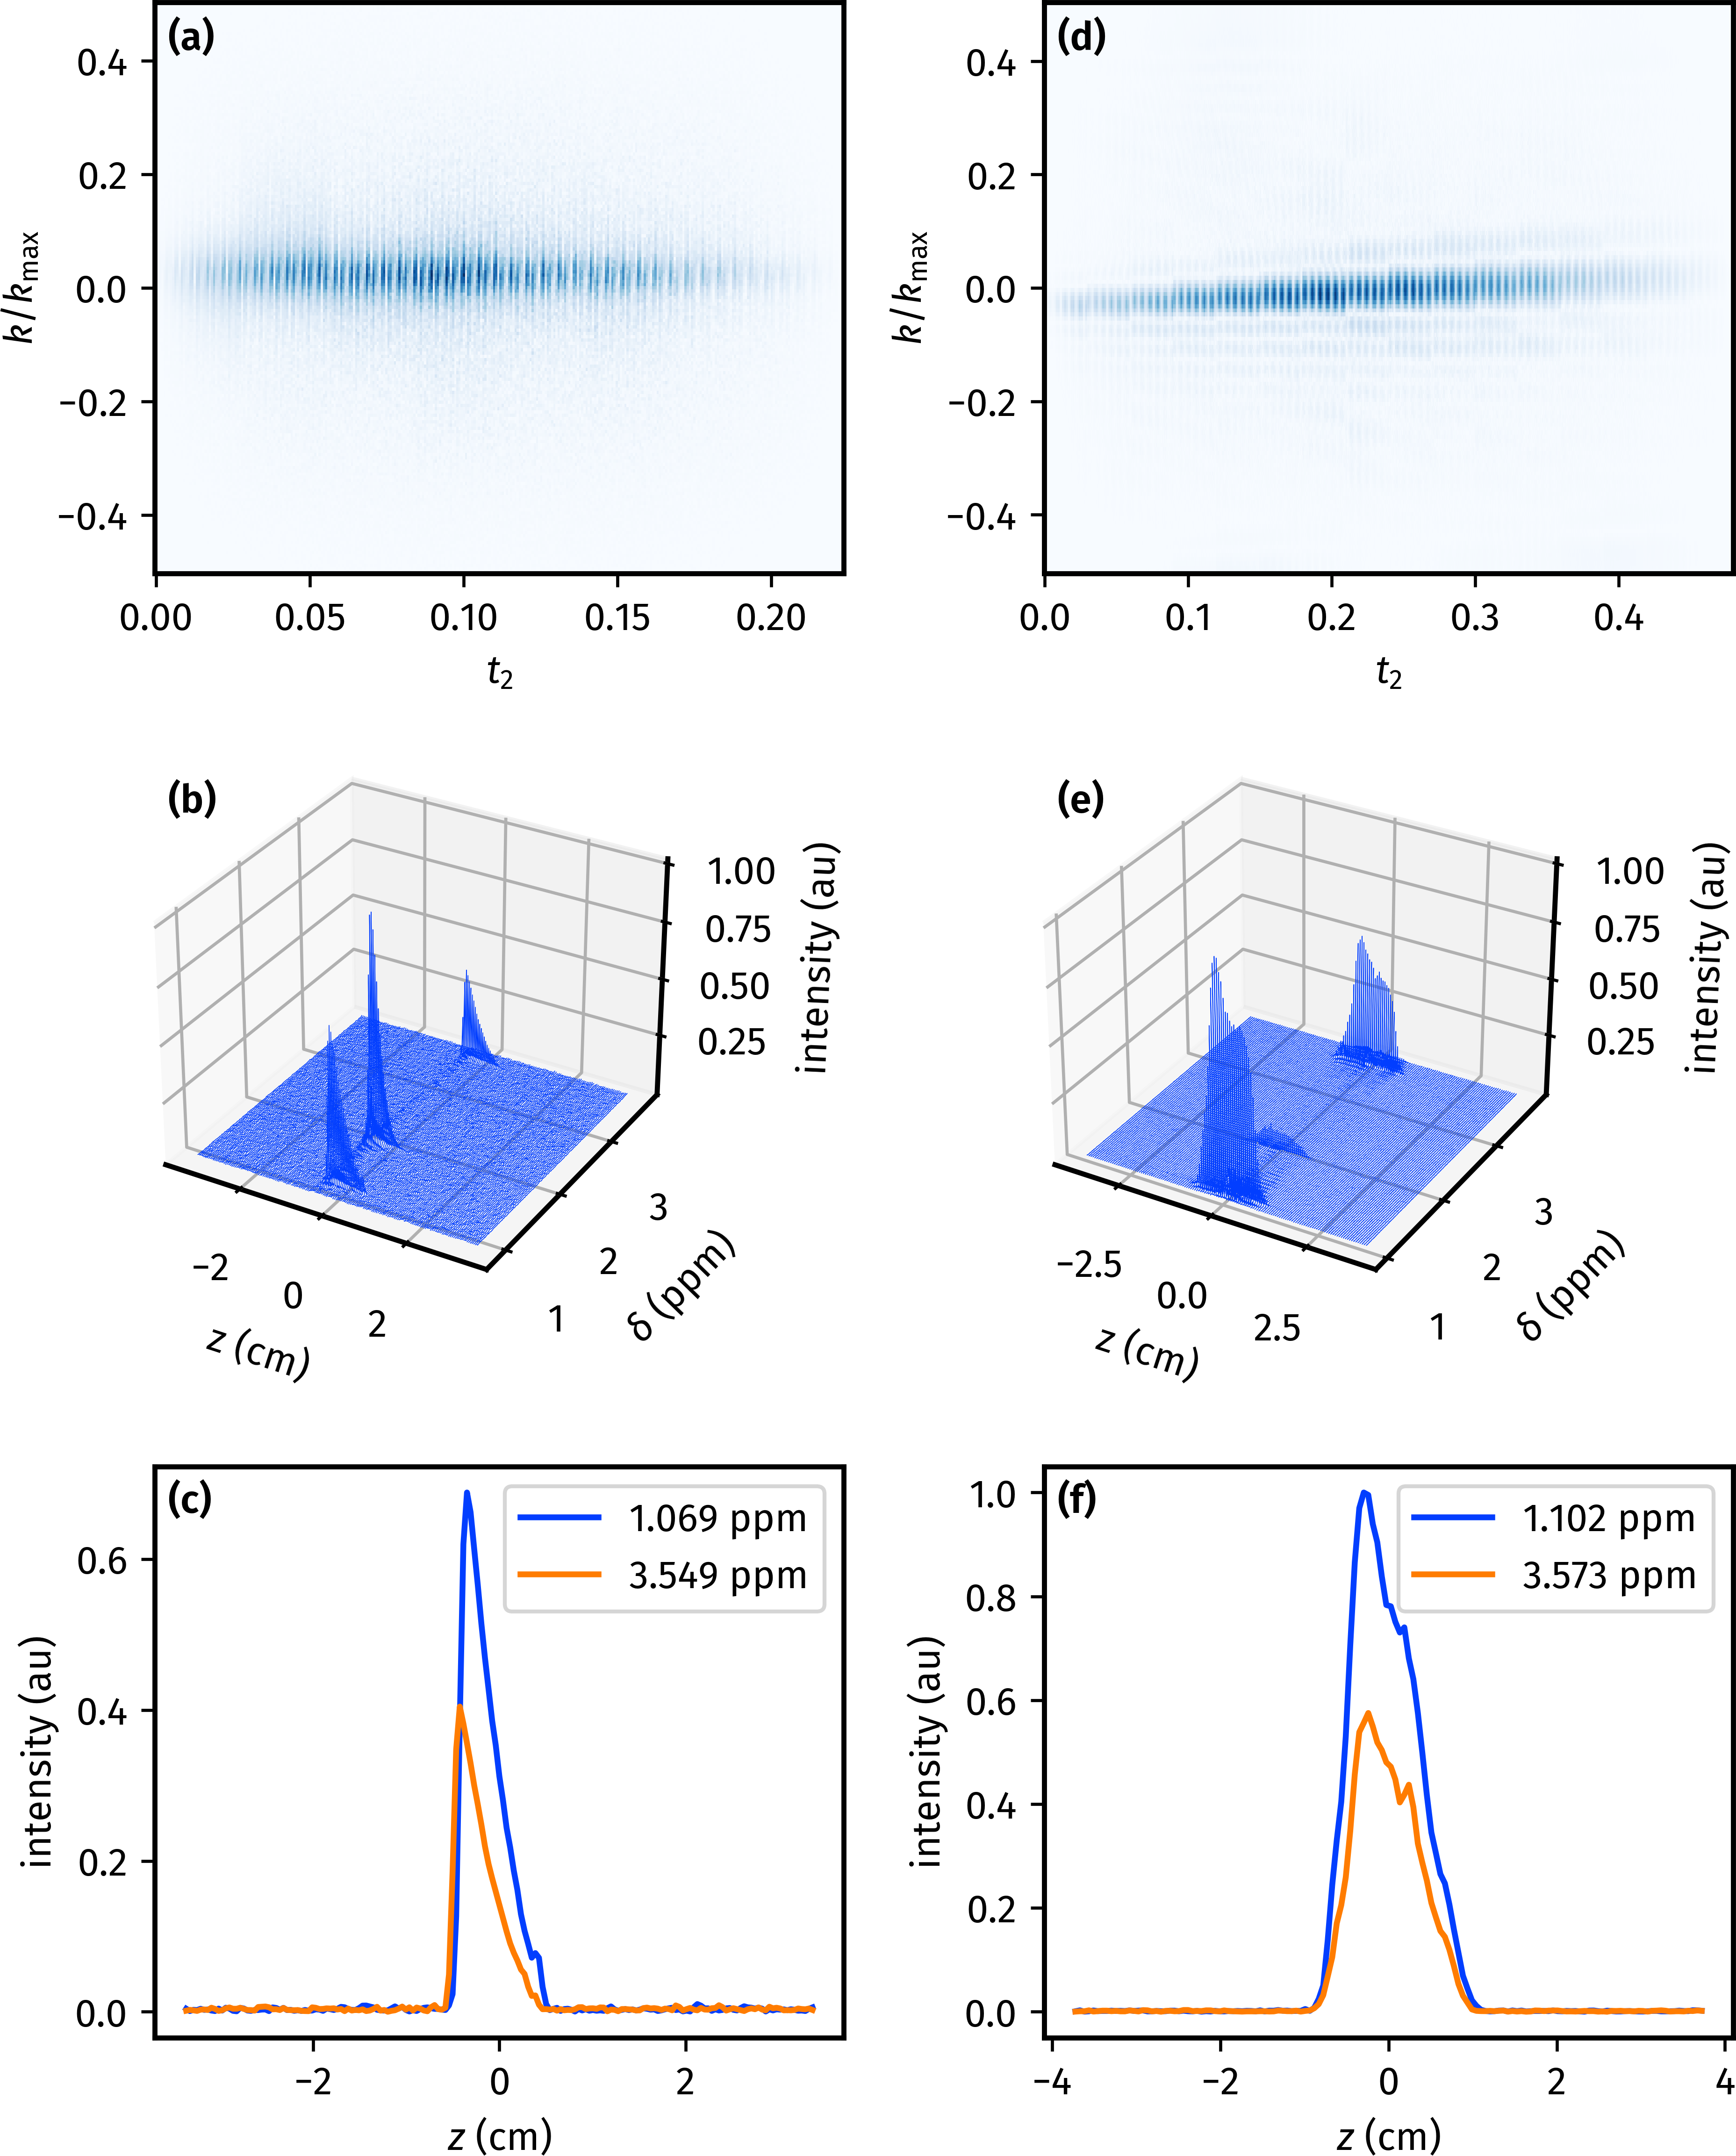
\includegraphics[]{pureshift/epsi_jnd_mf.png}%
    {\phantomsubcaption\label{fig:epsi_jnd_mf_jnd_kt}}%
    {\phantomsubcaption\label{fig:epsi_jnd_mf_jnd_zd}}%
    {\phantomsubcaption\label{fig:epsi_jnd_mf_jnd_trace}}%
    {\phantomsubcaption\label{fig:epsi_jnd_mf_mf_kt}}%
    {\phantomsubcaption\label{fig:epsi_jnd_mf_mf_zd}}%
    {\phantomsubcaption\label{fig:epsi_jnd_mf_mf_trace}}%
    \caption[Comparison of EPSI PSYCHE-iDOSY data acquired in Nantes and Oxford]{
        \textbf{(\subref{fig:epsi_jnd_mf_jnd_kt})--(\subref{fig:epsi_jnd_mf_jnd_trace})} EPSI PSYCHE-iDOSY data obtained by Corentin Jacquemmoz and Jean-Nicolas Dumez at the University of Nantes.
        The three plots respectively show the 2D raw $(k, t_2)$ data (after PSYCHE processing has been carried out); the Fourier transformed $(z, \delta)$ data; and the individual diffusion profiles for each peak.
        \textbf{(\subref{fig:epsi_jnd_mf_mf_kt})--(\subref{fig:epsi_jnd_mf_mf_trace})} The equivalent data which I recorded in Oxford.
        The central peak corresponds to \ch{HDO}; the Oxford sample used was drier and thus it is less intense in (\subref{fig:epsi_jnd_mf_mf_zd}) compared to (\subref{fig:epsi_jnd_mf_jnd_zd}).
        \datacode{6E-210426}
    }
    \label{fig:epsi_jnd_mf}
\end{figure}

In principle, the Fourier transformed $(z, \delta)$ plots should reveal a diffusion profile similar to that in Guduff et al.\autocite{Guduff2017CC}
This is the case for the Nantes data; in fact, it was possible to process this further to obtain a conventional 2D DOSY spectrum, where the diffusion coefficient for each component is extracted and plotted.
For the Oxford data, although the general \textit{form} of the curve is correct (in that there is a generally decreasing pattern), there are clearly `spikes' in the $(z,\delta)$ diffusion profiles.

My current best hypothesis is that these spikes are artefacts from unwanted CTPs which are ordinarily suppressed through spatial averaging, but are instead being refocused by the gradients during the EPSI acquisition.
This is supported by the fact that the Nantes data was acquired on a microimaging probe equipped with triaxial gradients, which allowed CTP gradients to be applied along the $x$- and $y$-axes (note that the PSYCHE gradient must still be applied along the $z$-axis).
Naturally, any artefacts dephased by these cannot be refocused by the $z$-gradients in the EPSI block.
On the other hand, the Oxford data was acquired on a Prodigy cryoprobe with only $z$-gradients.

The intensity of these `spike' artefacts can, in fact, be controlled by varying other acquisition parameters.
For example, increasing the EPSI gradient amplitude leads to increased artefacts (\cref{fig:epsi_parameters_moreepsi_kt,fig:epsi_parameters_moreepsi_trace}): this lends credence to the hypothesis above that the artefacts arise from refocused CTPs.
Notice also the appearance of signals at $k \neq 0$: this should not happen because in ultrafast experiments, the $k$-axis is proportional to the evolution frequency as a function of $z$ (i.e. indirect-dimension frequencies in a typical 2D experiment).
In a diffusion experiment, however, there is no frequency modulation in the indirect or spatial dimension, only amplitude modulation arising from diffusion attenuation; so, all signals should fall along $k = 0$.
In principle, the EPSI gradient could instead be reduced, but this has the drawback of lowering the resolution in the diffusion dimension.
Alternatively, when the PSYCHE gradient is increased, the artefacts seem to be reduced (\cref{fig:epsi_parameters_morepsyche_kt,fig:epsi_parameters_morepsyche_trace}).
However, this cannot be varied too much as the PSYCHE gradients are also responsible for the diffusion encoding (the value of $g$ in the Stejskal--Tanner equation are effectively derived from this).

\begin{figure}[htb]
    \centering
    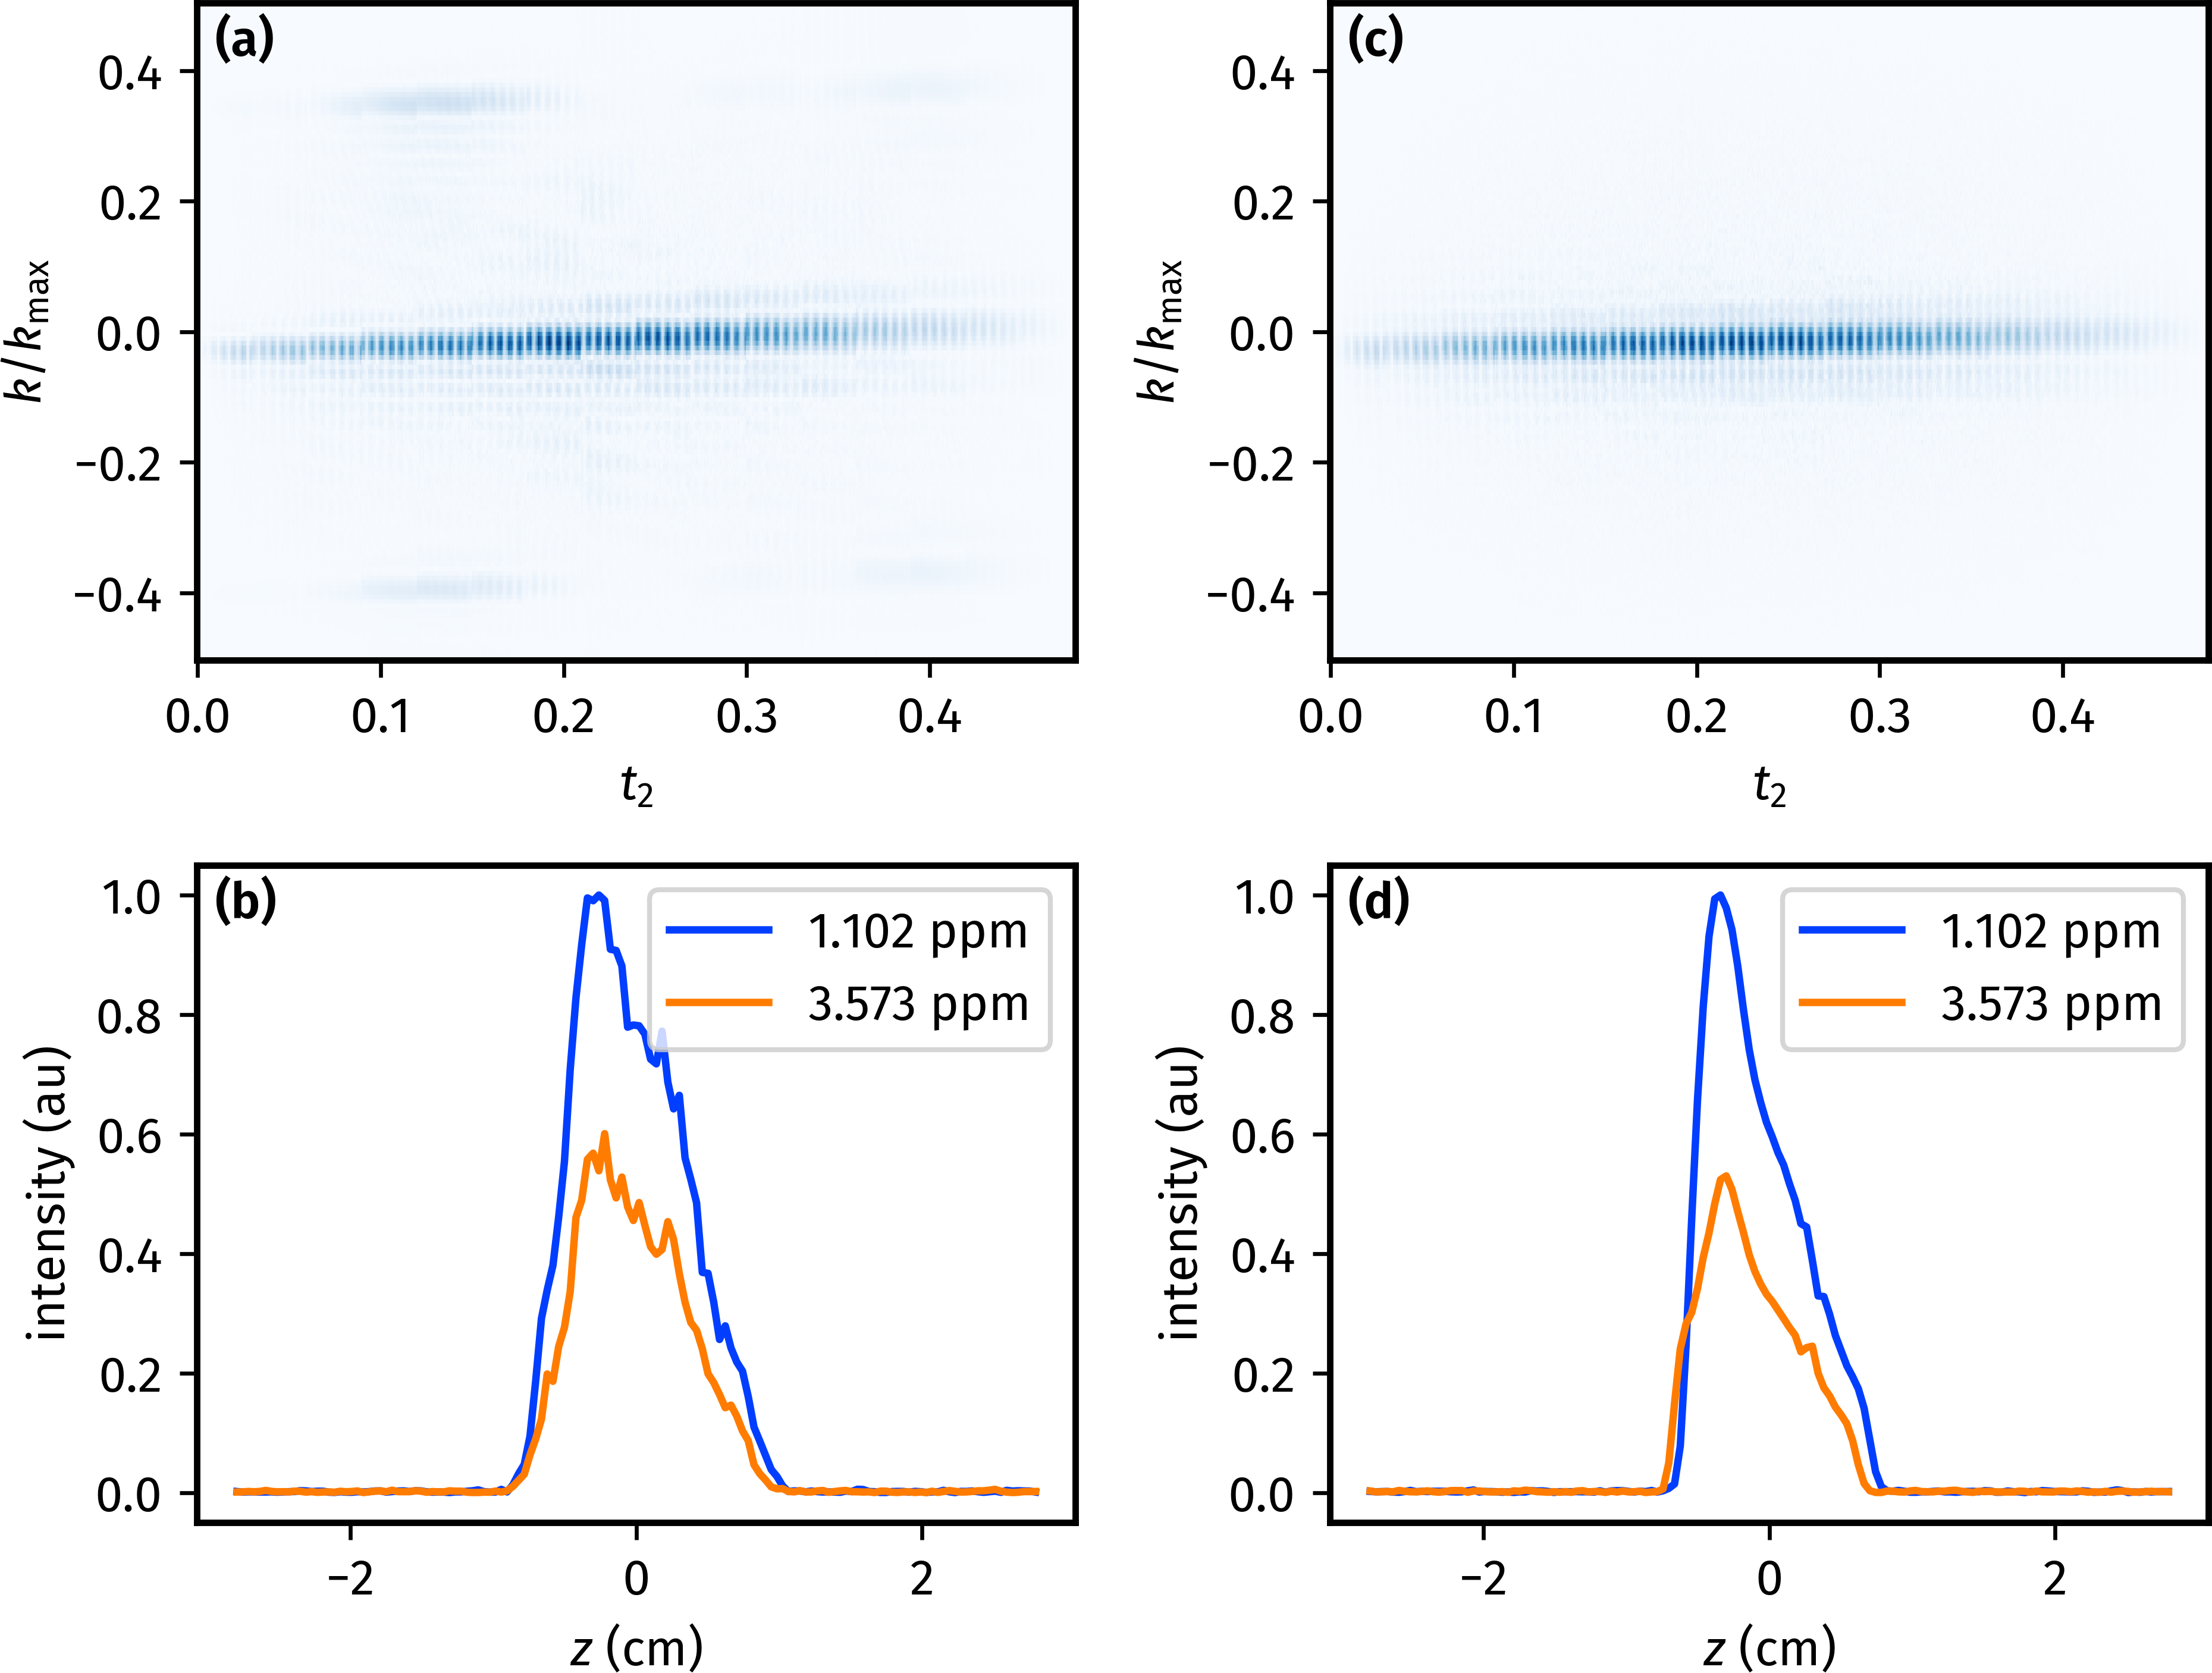
\includegraphics[]{pureshift/epsi_parameters.png}%
    {\phantomsubcaption\label{fig:epsi_parameters_moreepsi_kt}}%
    {\phantomsubcaption\label{fig:epsi_parameters_moreepsi_trace}}%
    {\phantomsubcaption\label{fig:epsi_parameters_morepsyche_kt}}%
    {\phantomsubcaption\label{fig:epsi_parameters_morepsyche_trace}}%
    \caption[Effects of varying acquisition parameters on ultrafast PSYCHE-iDOSY spectra]{
        \textbf{(\subref{fig:epsi_parameters_moreepsi_kt})--(\subref{fig:epsi_parameters_moreepsi_trace})} The same as in \cref{fig:epsi_jnd_mf_mf_kt,fig:epsi_jnd_mf_mf_trace}, but with the EPSI acquisition gradient increased to 32\% (from 24\% in the original).
        \datacode{6E-210426}
        \textbf{(\subref{fig:epsi_parameters_morepsyche_kt})--(\subref{fig:epsi_parameters_morepsyche_trace})} The same as in \cref{fig:epsi_jnd_mf_mf_kt,fig:epsi_jnd_mf_mf_trace}, but with the PSYCHE gradient increased to 5\% (from 3\% in the original).        
        \datacode{6E-210505}
    }
    \label{fig:epsi_parameters}
\end{figure}

Another possible reason for the artefacts is a potentially poorer $B_1$ homogeneity on the Oxford instrument.
However, a simple pulse--EPSI experiment (\cref{fig:zg_epsi}) shows that the $B_1$ spatial profile, though not perfect, is relatively uniform.

\begin{figure}[htb]
    \centering
    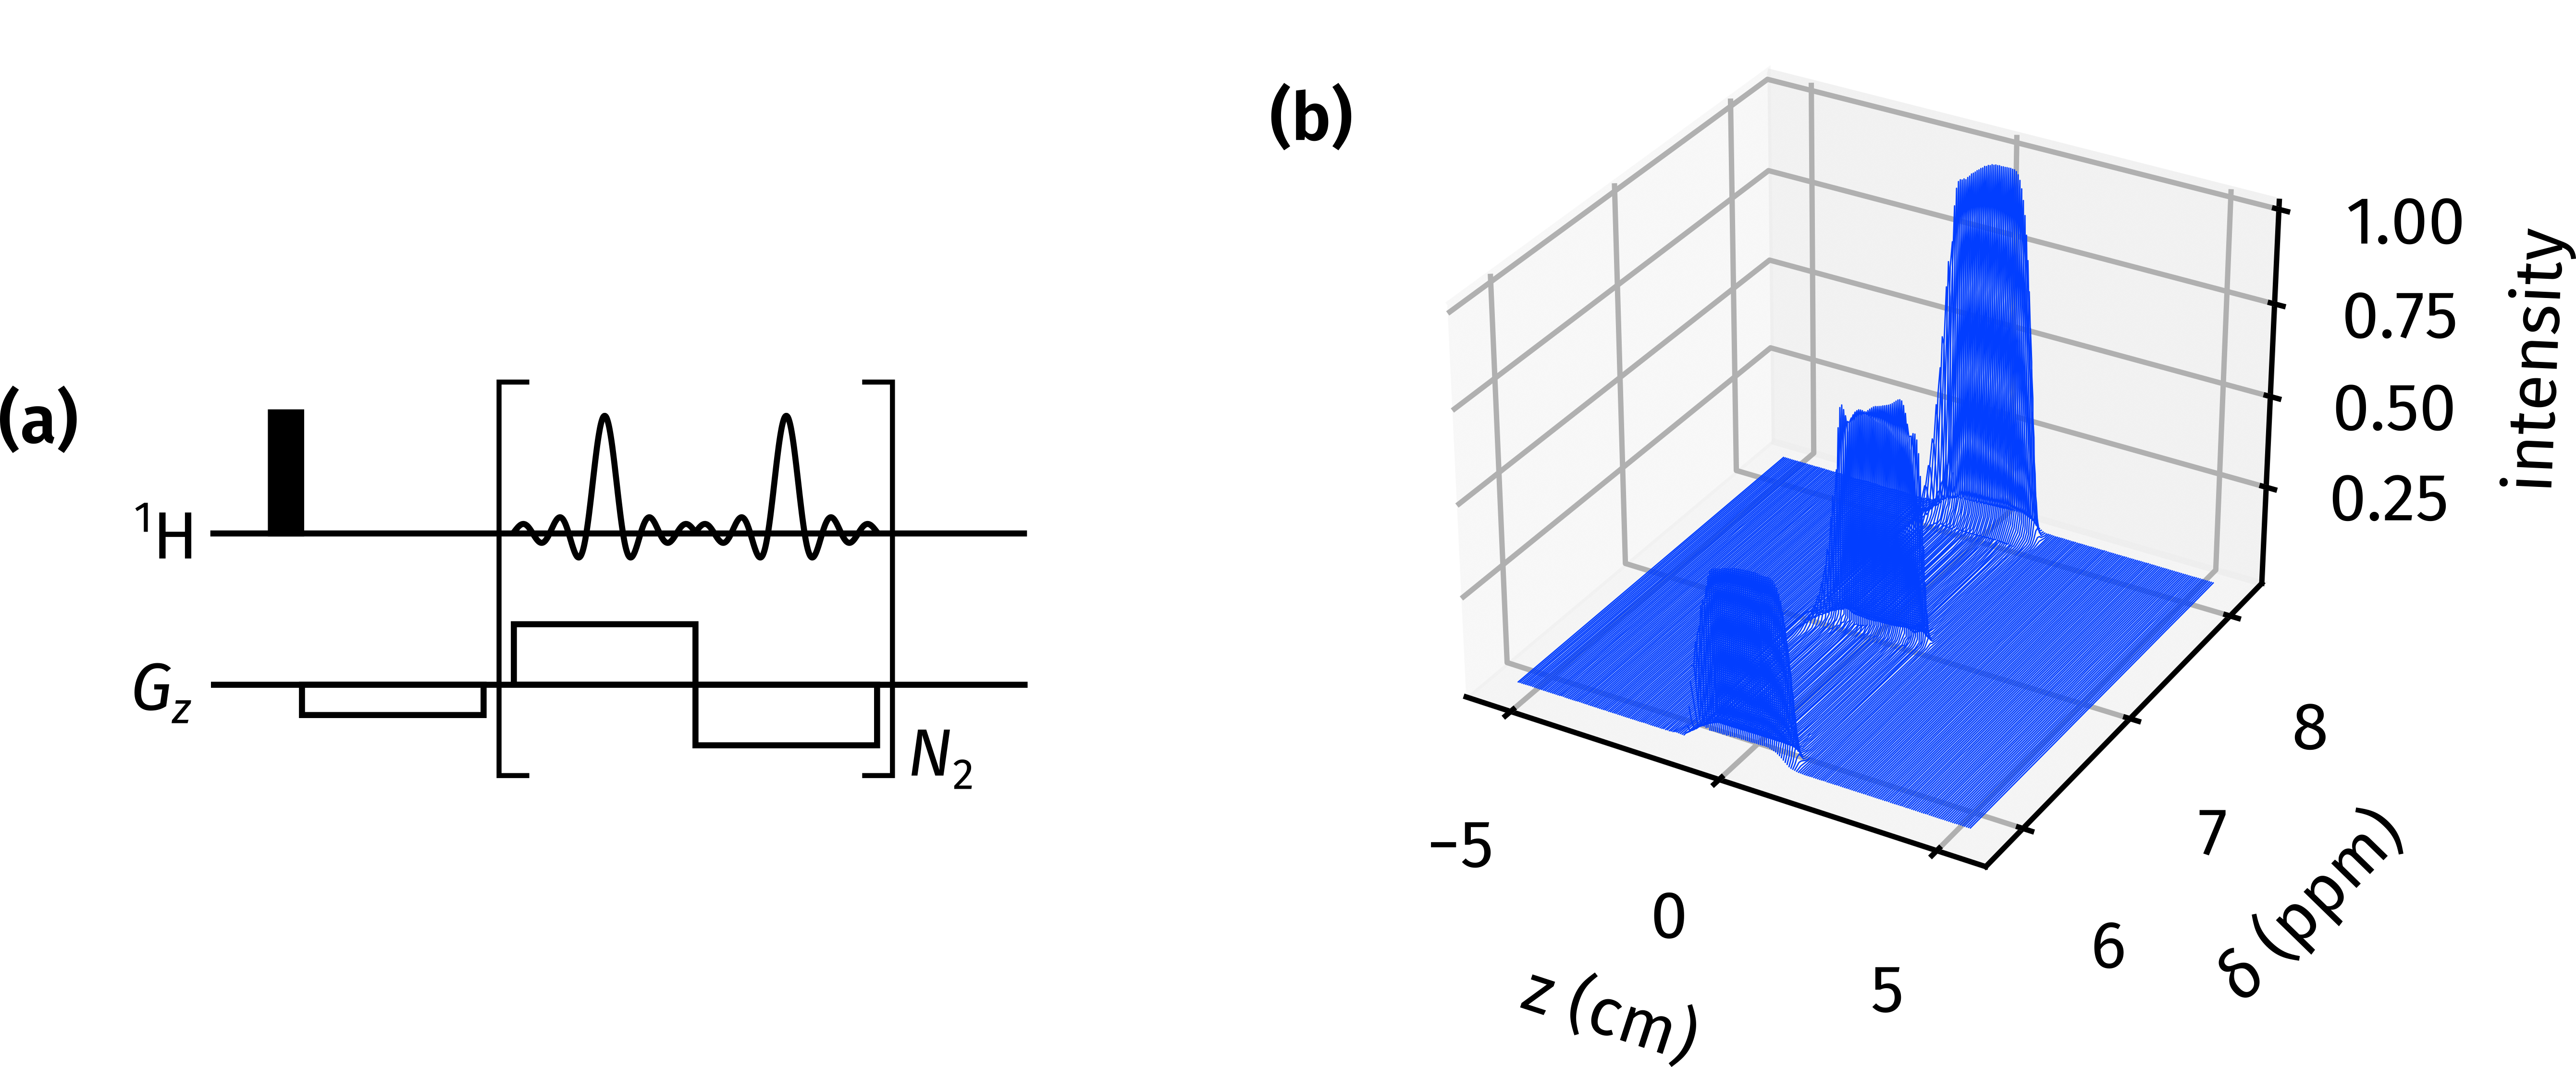
\includegraphics[]{pureshift/zg_epsi.png}%
    {\phantomsubcaption\label{fig:zg_epsi_pulseq}}%
    {\phantomsubcaption\label{fig:zg_epsi_spec}}%
    \caption[Pulse--EPSI pulse sequence and data]{
        \textbf{(\subref{fig:zg_epsi_pulseq})} Pulse--EPSI pulse sequence. The variation of the peak intensity along the $z$-axis directly corresponds to the $B_1$ spatial profile.
        \textbf{(\subref{fig:zg_epsi_spec})} The resulting data after Fourier transformation in both dimensions ($k \leftrightarrow z$ and $t_2 \leftrightarrow \delta$).
        \datacode{6E-210426}
    }
    \label{fig:zg_epsi}
\end{figure}

Curiously, \cref{fig:epsi_jnd_mf_mf_kt} shows that in the Oxford data, there is a progressive `shifting' along the $k$-axis in each PSYCHE chunk.
(The POISE optimisation in \cref{subsec:poise__epsi} was used to correct for the drifting \textit{within} each chunk, but cannot be applied to the overall drift after the concatenation of chunks.)
One possible explanation for this (Jean-Nicolas Dumez, private communication) is perhaps lingering effects from gradients applied during the pulse sequence, which have more time to dissipate when $t_1$ is longer.
This, however, does not have an appreciable impact on the data: it can be crudely corrected by circularly shifting the data along the $k$-axis by an appropriate amount, and Fourier transformation of the resulting data yielded effectively the same results.

All in all, it appears that the fundamental idea behind the ultrafast PSYCHE-iDOSY experiment is sound: the Nantes data is an excellent proof-of-principle.
However, the implementation of the sequence almost certainly needs to be optimised in order for high-quality data to be extracted.
An important subsequent step would then be to derive the appropriate form of the Stejskal--Tanner equation for extracting diffusion coefficients from the data.
Sadly, I simply did not quite have the time to pursue this in further detail.


\printbibliography[heading=subbibnumbered]{}
